%&pdflatex
%
%
%
%

% \documentclass[12pt]{article}
\documentclass[review,12pt]{elsarticle}

\usepackage{graphicx}
\usepackage{bm}
\usepackage{natbib}
\usepackage{xspace} % Incorporates correct optional space after commands
\usepackage{hyperref}

% Add line numbers
\usepackage[mathlines]{lineno} % Control line numbers

% Multipart figures
\usepackage{subcaption}  % "Newest" subfigure like package

% \oddsidemargin 0in
% \evensidemargin 0in
% \textwidth= 6.5in
% \topmargin -0.50in
% \textheight 9in

\usepackage{ifpdf} % For declaring rules for graphics below

\usepackage{latexsym,amssymb,amsmath,color}
% \newcommand{\revised}[1]{\textcolor{blue}{{#1}}}
% \newcommand{\comment}[1]{\textcolor{red}{{#1}}}
% \newcommand{\alert}[1]{\textbf{\textcolor{red}{{#1}}}}
\newcommand{\be}{\begin{equation}}
\newcommand{\ee}{\end{equation}}
\newcommand{\xxi}{\vec{\xi}}
\newcommand{\xxii}{\xxi^{(\scriptscriptstyle{-}\scriptstyle{i})}}
\newcommand{\var}[1]{{\mathrm{Var}}\left[ {#1} \right]}
\newcommand{\ip}[2]{\left( {#1}, {#2} \right)}
\newcommand{\U}{\mathcal{U}}
\newcommand{\normim}[1]{\left\| {#1} \right\|_{\scriptscriptstyle L^{2}(\Omega^{*})}}
\newcommand{\avemu}[1]{\mathrm{E}\left({#1}\right)}
\newcommand{\ave}[1]{\left\langle {#1} \right\rangle}
\newcommand{\prob}[1]{\mathrm{Prob}\left\{ {#1} \right\}}
\newcommand{\ind}[1]{\mathrm{\chi}_{\scriptscriptstyle {#1} }}
\newcommand{\NISP}{\mathcal{S}}
\newcommand{\ipmu}[2]{\left( {#1}, {#2} \right)_\mu}
\newcommand{\norm}[1]{\left\| {#1} \right\|_{\scriptscriptstyle L^{2}(\Omega)}}
\newcommand{\pard}[2]{\frac{\partial{#1}}{\partial{#2}}}
\def\xbold{{\vec{x}}}
\renewcommand{\vec}[1]{{\mathchoice
                     {\mbox{\boldmath$\displaystyle{#1}$}}
                     {\mbox{\boldmath$\textstyle{#1}$}}
                     {\mbox{\boldmath$\scriptstyle{#1}$}}
                     {\mbox{\boldmath$\scriptscriptstyle{#1}$}}}}

\newcommand{\pd}{\pard}
\newcommand{\geoclaw}{{\sc GeoClaw}\xspace}
\newcommand{\tohoku}{T\={o}hoku\xspace}
\newcommand{\dx}{\ensuremath{\Delta x}}   % Delta x
\newcommand{\dy}{\ensuremath{\Delta y}}   % Delta y
\newcommand{\dt}{\ensuremath{\Delta t}}   % Delta t
        
\journal{Ocean Modelling}

\begin{document}

\ifpdf
\DeclareGraphicsExtensions{.pdf, .png, .jpg, .tif}
\else
\DeclareGraphicsExtensions{.png, .jpg, .tif, .eps}
\fi

\begin{frontmatter}

\title{Uncertainty Quantification and Inference of Manning's Friction Coefficient using DART Buoys Data during
\tohoku Tsunami}
\date{\today}

\author[kaust1]{Ihab Sraj}
\author[ut]{Kyle T. Mandli}
\author[duke,kaust2]{Omar M. Knio}
\author[ut]{Clint N. Dawson}
\author[kaust1,kaust2]{Ibrahim Hoteit\corref{cor1}}
\ead{ibrahim.hoteit@kaust.edu.sa}
%\ead{Division of Physical Sciences and Engineering, King Abdullah University for Science and Technology, Thuwal, Saudi Arabia}
\address[kaust1]{Division of Physical Sciences and Engineering, King Abdullah University for Science and Technology, Thuwal, Saudi Arabia}

\address[ut]{Institute for Computational Engineering and Science, University of Texas at Austin, 201 E 24th ST. Stop C0200, Austin, TX 78712-1229, USA}
\address[duke]{Department of Mechanical Engineering and Materials Science, Duke University, 144
Hudson Hall, Durham, North Carolina 27708, USA}
\address[kaust2]{Division of Computer, Electrical and Mathematical Sciences and Engineering, King Abdullah University for Science and Technology, Thuwal, Saudi Arabia}
\cortext[cor1]{Corresponding author}
\date{\today}

\begin{abstract}

Tsunami computational models are employed to explore multiple flooding
scenarios and to predict water elevations.  However, accurate estimation of
water elevations  requires accurate estimation of many model parameters, in
particular the Manning's $n$ friction coefficient.  Our objective is to
develop an efficient approach for the  uncertainty quantification and inference
of the Manning's $n$ coefficient which we characterize here by three different
parameters as being constant over three different regions: $n_1$ on-shore,
$n_2$ near-shore and $n_3$ deep-water.  We use Polynomial Chaos (PC) to build an
inexpensive surrogate for the  \geoclaw model and then employ Bayesian inference
to estimate  and quantify the uncertainties to those uncertain parameters using
the DART buoy data collected during the \tohoku tsunami.  The surrogate model
significantly reduces the computational burden of the Markov Chain Monte-Carlo
(MCMC)  sampling of the Bayesian inference. The PC surrogate is also used to
perform a sensitivity analysis.  Our results indicate that Manning's $n$
coefficients have a Maximum-A-Posteriori (MAP) values of $n_2=0.011$ and
$n_3=0.180$, while for $n_1$ no meaningful MAP value can be determined from the
available data.

\end{abstract}

\begin{keyword}
tsunami \sep Manning's $n$ friction coefficient \sep sensitivity analysis \sep polynomial chaos \sep Bayesian inference
\end{keyword}

\end{frontmatter}
\linenumbers

% \renewcommand{\thefootnote}{\fnsymbol{footnote}}

\begin{center}
\begin{Large}
{\bf Polynomial Chaos for the Estimation of Manning's Friction}\\

\end{Large}
\bigskip
\bigskip
Ihab Sraj$^1$, Kyle Mandli$^2$, Ibrahim Hoteit$^1$, \& Clint Dawson$^2$\\
\bigskip
$^1$Department of Physical Sciences and Engineering,
King Abdullah University for Science and Technology, Thuwal, Saudi Arabia \\
$^2$Institute for Computational Engineering and Science\\
University of Texas at Austin\\
Austin, TX 
\end{center}

\vspace{5.5cm}

\begin{tabbing}
Corresponding Author: \hspace{5mm} \=  \\
       \> Department of Physical Sciences and Engineering \\
       \> King Abdullah University for Science and Technology \\
       \> Thuwal, Saudi Arabia\\
       \> \\
Phone: \>  \\
Fax:   \>  \\
Email: \>    \\
\\
Submitted to: \> {\it TBD} \\
\> \today \\
\\
Revised: \>  

\end{tabbing}





% \clearpage

%!TEX root = paper.tex

\section{Introduction} \label{sec:intro}

Tsunamis in the past decade have been responsible for some of the most  deadly
and costly natural disasters ever recorded. Coastal communities have faced this
hazard by assessing the risk they pose, attempting  to make informed decisions
about the likelihood that such an event would  occur.
Toward this goal, computational models of  tsunami events are often
employed to explore multiple scenarios and to predict the water elevation
caused by the tsunamis. The accurate prediction  of water elevations, however,
requires accurate estimation of many model parameters that are either measured
directly, defined empirically, or estimated from a collection of observed data.
Unfortunately, since tsunami events are relatively rare,  there is a large
uncertainty in the input data for these computational  models ranging from
effects of the domain, such as bathymetry and friction parameterizations,  to
the earthquake source.  In this study, we aim to estimate the Manning's $n$
friction coefficient, a parameterization of the effect of bottom friction 
commonly used in tsunami models.  We aim at quantifying the uncertainty in the 
predicted water elevation  and employ a Bayesian inverse modeling approach to 
estimate the Manning's $n$ coefficient using observations of water elevation 
measured during a tsunami event.

Previous work concerning uncertainty quantification in tsunami modeling has been primarily 
focused on constraining the likely earthquake source models (see
for example \cite{MacInnes:2013cr}).  A similar approach for landslide-generated
tsunami was presented in Sarri \emph{et al.}~\cite{Sarri2012}, by building a statistical surrogate
using an emulator. The implemented emulator was based on a Gaussian
process that requires using a combination of prior knowledge about the simulator
and appropriate choices of functions and parameters. Their work was presented as
a proof-of-concept case study where they only performed basic statistical and
sensitivity analysis.  Changes to the friction parameterization has been shown in 
the past to lead to significant changes in predicted inundation levels \cite{Myers:2001el, 
Jakeman:2010hk}, but these previous studies were limited in range and spatial variation of the values used in the parameterization.  
In a recent work, Mayo \emph{et al.}~\cite{Mayo:2014} reformulated a statistical data assimilation method
generally used in the estimation of model states to estimate the Manning's $n$
coefficient. They used a low-dimensional representation of
Manning's $n$ coefficients and recovered it by assimilating synthetic water elevation data using tidal simulations.

In this work, we focus our attention on the uncertainty in the friction
parameterization used in tsunami simulations. We present a three-parameter 
representation of Manning's $n$ coefficient and an efficient method
to estimate this representation using measured water elevation data. The method proposed here 
is based on recent developments in Uncertainty Quantification (UQ) methods that allow 
probing of the sensitivity of realistic tsunami  models to uncertain parameters
without modifying the forward model and inferring those parameters
from a number of observations.  In particular, we implement an inverse modeling
approach that relies on a Bayesian inference technique.  We resort to
Polynomial Chaos (PC) expansions to build a surrogate model ~\cite{Najm:2009,Alexanderian2012,Elsheikh2014,Young2013}
of the response of the tsunami predicted using the \geoclaw model.
The PC surrogate enables us to avoid using the forward model in
the Bayesian inference, thus dramatically reducing the cost of sampling the
posterior distribution.

PC expansions have been developed and applied in the engineering community to
quantify uncertainties in numerical simulations.  The main advantage of
using PC expansions is the ability of efficiently propagating input uncertainties through 
large, complex and non-linear models leading to the corresponding output uncertainties. 
Several studies already investigated the efficiency of PC expansions for 
UQ in oceanic simulations~\citep{thacker2012,ashwanth2010,Alexanderian2012,sraj:2013a}. 
Recently, PC was combined with Bayesian inference to estimate the wind drag coefficient 
using temperature data collected during Typhoon Fanapi 2010. The same problem was 
solved using two different techniques: the adjoint method and Markov Chain Monte Carlo
(MCMC)\cite{sraj:2013a,sraj:2013b}.

In this work, we follow a similar procedure as in \cite{sraj:2013a,sraj:2013b}
to estimate Manning's $n$ coefficient using the \tohoku tsunami
event as a case-study. The quantity of interest is taken to be the water surface
elevation and is compared to the available NOAA Deep-ocean Assessment and
Reporting Tsunamis (DART) buoys.  The forward model runs are performed using the
\geoclaw package following the setup in MacInnes \emph{et al.}~\cite{MacInnes:2013cr}.

The structure of this manuscript is as follows. First, we describe our case-study, the \tohoku tsunami,
summarize the forward simulations setup, and present the DART buoys observational data
in Section~\ref{sec:tohoku}. Section~\ref{sec:manning} discusses the uncertainties 
of the Manning's $n$ coefficient to motivate the UQ problem and propose a three-parameter representation of $n$. 
Section~\ref{sec:formu} presents the two main methods employed in the UQ analysis:
Bayesian inference that brings together observations 
and model results (Section~\ref{sec:inference}) 
and PC expansions that are used to build the surrogate model (Section~\ref{sec:uqpce}). Section~\ref{sec:results} describes the main results in 
three subsections: first, we perform error and convergence studies
as evidences that the PC surrogate is a faithful 
representation of the \geoclaw model; second, we use the PC surrogate to 
perform a statistical analysis and compute the  sensitivity of simulated water elevations
to the uncertain input parameters; and third, we present the results of the
posterior distributions obtained using Bayesian inference by MCMC. A discussion of our findings and methodology is finally presented in Section~\ref{sec:conc}.

%\comment{
%\begin{itemize}
%    \item There are two places where we refer to the parameterization as three-dimensional, I am not sure if this is really three-dimensional.  I know that we are using depth contours but the parameterization is two-dimensional.  I have a feeling that readers would take issue with this.
%    \item Ihab: the representation is 3D meaning we used three different values of n in three regions. The same concept was presented in Mayo paper where they did 2D representation.
%    \item I think the order here needs to be revised to talk about the forward model and the equations we are solving first since the Manning's $n$ discussion refers to equations there. 
%    \item Ihab: Our main objective is to show the UQ techniques and how they work. The equations are known and we do not need to stress on them. We can even remove the whole equation or forward model section.
%\end{itemize}
%}

%!TEX root = paper.tex
\section{The \tohoku Tsunami} 
\label{sec:tohoku}

The \tohoku earthquake and tsunami of 2011 have been the subject of a number of
studies due to the wealth of observational evidence and severity of the tsunami~\cite{Kawase2014}.
The earthquake itself had an estimated magnitude of $\text{M}_\text{w}$ 9.0 and
caused massive devastation across Japan. The source of the earthquake (epicenter)
was located approximately 72 km east of \tohoku as indicated 
in Figure~\ref{fig:ceofs}. In our case study, the
simulation used is based on work done in \cite{MacInnes:2013cr} and modified to 
use the specified variable friction field. Hereafter, we briefly describe the
forward computational model, \geoclaw, the  simulation setup used in the
uncertainty analysis, and finally present the observations from NOAA DART buoys.


\subsection{\geoclaw} \label{ssub:geoclaw}
The \geoclaw software package uses a finite volume, wave-propagation approach as
described in \cite{LeVeque:1997eg} to solve the two-dimensional shallow water
equations (SWE):

\begin{equation} \label{eq:swe}
    \begin{aligned}
    &\pd{}{t} h + \pd{}{x} (hu) + \pd{}{y} (hv) = 0, \\
    &\pd{}{t}(hu) + \pd{}{x} \left(hu^2 + \frac{1}{2} g h^2 \right ) + \pd{}{y} (huv) = ~~ fhv - gh \pd{}{x} b - C_f |\vec{u}| hu, \\
    &\pd{}{t} (hv) + \pd{}{x} (huv) + \pd{}{y} \left (hv^2 + \frac{1}{2} gh^2 \right) = -fhu - gh \pd{}{y} b - C_f |\vec{u}| hv,
    \end{aligned}
\end{equation} 
where $h$ is the depth of the water column, $u$ and $v$ the velocities in the 
longitudinal and latitudinal directions respectively, $g$ the acceleration due 
to gravity, $b$ the bathymetry, $f$ the Coriolis parameter, and $C_f$ the bottom 
friction coefficient.  
%As is common in tsunami modeling, $C_f$ is calculated 
%given a Manning's $n$ parameterization such that:
%\begin{equation}
%    C_f = \frac{g n^2}{h^{4/3}},
%\label{eq:coef}
%\end{equation}
%where $n$ is an empirically determined parameter known as Manning's $n$.  

The primary computational kernel in \geoclaw is the evaluation of the solution
to the Riemann problem at each grid cell interface.  The Riemann solver used
includes the ability to handle inundation (wet-dry interfaces), well-balancing,
even when the momentum is non-zero, and entropy corrections
\cite{George:2008aa}.

One of the unique features of \geoclaw is the ability to adaptively refine the
grids used for the computation, essentially following a region of interest as
time progresses (in this case, the disturbance in the surface height).
To this end, \geoclaw implements the schemes in \cite{Berger:1984ui,Berger:1998aa}
as described in detail in \cite{Berger:2011du} in the case of tsunami
modeling.

For the simulations presented, refinement thresholds were used that matched what
was presented in \cite{MacInnes:2013cr}.  As was done there, four levels of
refinement were used starting with a resolution of 1 degree in both the
latitudinal and longitudinal directions down to 0.5' resolution (approximately
900 meters) located around the observation locations.  The tolerance for the
refinement criteria for sea-surface anomaly was 0.02 meters.

\subsection{DART Buoy Observations}

The observations used in this study are from the Deep-ocean Assessment and
Reporting of Tsunamis (DART) buoy system developed and maintained by the
National Oceanic and Atmospheric Administration (NOAA).  The purpose of the
network is to provide early-warning detection and forecasting of tsunami
propagation in the Pacific Ocean \cite{Milburn:1996wm}.  The DART buoys closest
to the earthquake source of the \tohoku tsunami were buoys 21401, 21413, 21418,
and 21419 whose locations are shown in Figure~\ref{fig:setup_buoy_locations} and
whose de-tided water surface elevation data for the event are shown in
Figure~\ref{fig:setup_buoy_data}. The time $t=0$ is set to be the start of the
earthquake and is recorded every 15 seconds during the first few minutes of the
event, otherwise recording every minute when triggered (a tsunami has occurred)
or every 15 minutes when not.  We can see that the primary tsunami
waves generated reach the gauges between 40 minutes and 2 hours after the
earthquake.  The large spikes later in time present in the data at gauge 21418
are data anomalies and not subsequent tsunami waves as observed in \cite{MacInnes:2013cr}.

\subsection{Bathymetry and Earthquake Source Model}

The bathymetry used in the simulation is a combination of ETOPO 1' and 4'
accurate bathymetry for the region \cite{Amante:2009ud}.  Finer bathymetry was
used in the study done in MacInnes \emph{et al.} in order to match the on-shore
inundation levels.  In the current study this bathymetry was excluded since we
are only concentrating on the data from the DART buoys. The bathymetry and 
topography of the considered regions are shown in Figure~\ref{fig:setup_buoy_locations}.

The earthquake source model that was used is due to Ammon \emph{et al.}
\cite{Ammon:2011dm} who used inversion of the seismic waves to reconstruct the
rupture.  This model was chosen as it provides a rupture reconstruction based on
established techniques and did include tsunami inversion data.  The
latter may introduce bias into the reported results of this study and was consequently ignored.
As discussed in MacInnes \emph{et al.}, the source models used do not include
rupture timing which could have an impact on the accuracy of the simulation.


\section{Manning's $n$ Friction Coefficient} \label{sec:manning}

Manning's $n$ law provides a relationship between the friction coefficient
$C_f$ appearing in the SWE governing tsunamis (Equation \ref{eq:swe}) and 
the empirically derived roughness parameter $n$:

\begin{equation}
    C_f = \frac{g n^2}{h^{4/3}},
\label{eq:coef}
\end{equation}
The value of $n$ may vary both spatially and temporally due to changes in the
bottom roughness from wave action and other processes.  For tsunami modeling it
is a common practice to assume a single value of Manning's $n$ for the areas
that are initially below sea-level; while satellite images and 
land-use data are sometimes used to determine the coefficient in areas above sea-level.  
Both above and below sea-level, this process has several sources of uncertainty, all
of which can have an impact on the quantities of interest in tsunami modeling.   
MacInnes \emph{et al.}, for instance, found that adopting a uniform value 
of $n = 0.025$ everywhere leads to poor performance of the forward model's predicted 
inundation levels.  To address this they used $n = 0.035$ in the Sendai plane to 
account for land-uses such as pasture, farmland, and rice paddies.  We aim to address such
uncertainties in a systematic way in order to better study risk assessments.

The direct result of the uncertainty in the Manning's $n$ coefficient leads to
uncertainties in water elevation,
especially in the most crucial area in risk assessments, the near-shore. In 
addition,  the prediction of this and other quantities of interest is often highly 
sensitive to changes in these uncertain parameters.  Therefore, we seek to 
quantify the parametric uncertainty due to the uncertainty in the Manning's $n$ 
friction coefficient by characterizing the spatial variability using
iso-baths to define distinct regions in the domain that are characterized by a
single Manning's $n$ coefficient.  In this study three regions are used, an
on-shore region (initially above sea-level), a near-shore region (between
sea-level and the 200 meter iso-bath), and the deep-water region (deeper than
200 meters), whose Manning's $n$ coefficient is denoted by $n_1$, $n_2$, and $n_3$ respectively 
as shown in Figure~\ref{fig:ceofs}. To quantify the uncertainties
in these three parameters we employ Polynomial Chaos (PC) 
expansions as used in \cite{sraj:2013a,sraj:2013b}.  The method and its 
application to our problem is
described in Section~\ref{sec:uqpce}.  To represent the initial uncertainty in the
Manning's $n$ coefficients an uninformative uniform distribution was assumed as 
the prior with physically relevant values of $n$ sampled from the interval 
$n \in [0.005-0.2]$.
\section{Formulation}
\label{sec:formu}
In this section, we first present the Bayesian approach to inverse problems 
and its application to our problem of inferring the Manning's $n$ coefficients.
We also introduce
a Polynomial Chaos method used for forward uncertainty propagation, and 
for accelerating the Bayesian inference.
\subsection{Bayesian Inference}
 \label{sec:inference}
 
Bayesian inference is a statistical approach to inverse problems
that has recently gained great interest in different applications, including
ocean~\citep{Alexagnderian2011a,Zedler2012,sraj:2013a}
climate~\citep{OlsonEtAl2012} and geophysical~\citep{Malinverno2002} modeling.
The key idea in this approach is to express all forms of uncertainty
in terms of canonical random variables. The first step in Bayesian inference 
is to formulate the forward problem (response surface/model) using 
a suitable likelihood function and a product of conditional probability densities. 
The prior distributions over the unknown parameters of the model
are then formulated using the best available knowledge of the parameters.  Given some observation data, Bayes rule 
is then used to computer the posterior distribution for these unknown parameters
\citep{sivia}. We briefly review this approach below.
\subsubsection{Formalism}

Let $\vec{d}=(d_1,...,d_m)^T$ be a vector of observation data and $\vec{\theta}=(\theta_1,...,\theta_n)^T$ be a vector of model parameters or inputs. We consider a forward model $\vec G$ that predicts the data as function of 
the parameters such that:

\begin{equation}
\vec d \approx \vec{G}( \vec \theta).
\end{equation}
Applying the Bayes' rule yields:

\begin{equation}
 \Pi(\vec{\theta}| \vec d) \propto 
 L(\vec d | \vec{\theta}) \ q(\vec{\theta}), 
\label{eq:bayes}
\end{equation}
where $q(\vec{\theta})$ is the prior of $\vec{\theta}$, representing the \emph{a priori} knowledge
about the parameters; 
$L(\vec d| \vec{\theta})$ is the likelihood function representing
the probability of obtaining the data given the set of parameters $\vec{\theta}$;
and finally $\Pi(\vec{\theta}| \vec d)$ is the posterior,
representing the probability of occurrence of $\vec{\theta}$ given the data $\vec d $.

To formulate the likelihood function, we let $\vec \epsilon = \vec d - \vec{G}$
represent the discrepancy between the model and observations.
Here, the components of $\vec \epsilon $ are assumed to be i.i.d. random variables with density $p_{\epsilon}$.
The likelihood function can thus be written as:

\begin{equation} 
L(\vec d |  \vec{\theta}) 
= 
\prod_{i=1}^m  
p_\epsilon (d_i - G_i(\vec \theta)), 	
\label{eq:likelihood}
\end{equation}
where $m$ is the number of observations (dimension of $\vec{d}$).

In our application, we assume that the errors $\epsilon_i$ are independent
and normally distributed with mean
zero and variance $\sigma^2$, i.e. $\epsilon_i \sim N(0,\sigma^2)$. 
While in general $\sigma^2$ (the variance of the noise in the measured data) depends on the observations, in our case we assume that the error
amplitude is generally small and does not change throughout space and time.
Consequently, one may assume a single $\sigma^2$ value in Equation~\eqref{eq:likelihood},
resulting in:

\begin{equation} 
L(\vec d |  \vec{\theta}) 
= 
\frac{1}{\sqrt{2 \pi \sigma^2}}\prod_{i=1}^m   
\exp \left\lbrace \frac{-(d_i - G_i(\vec \theta))^2}{2 \sigma^2} \right\rbrace. 	
\label{eq:likelihood2}
\end{equation}
The joint posterior from Bayes' rule can thus be given as:

\begin{equation} 
\Pi(\vec{\theta}| \vec d)
\propto
\frac{1}{\sqrt{2 \pi \sigma^2}}   \prod_{i=1}^m  
\exp \left\lbrace \frac{-(d_i - G_i(\vec \theta))^2}{2 \sigma^2} \right\rbrace  
\prod_{i=1}^n q(\theta_i).
\end{equation}
Since $\sigma^2$ is unknown \emph{a priori} we treat it as a hyper-parameter.
In other words, $\sigma^2$ becomes an additional parameter for Bayesian inference and  
therefore endowed with a prior which is updated based on available observations. In this 
case the joint posterior is finally expressed as:

\begin{equation} 
\Pi(\vec{\theta},\sigma^2 | \vec d)
\propto
\frac{1}{\sqrt{2 \pi \sigma^2}}   \prod_{i=1}^m  
\exp \left\lbrace \frac{-(d_i - G_i(\vec \theta))^2}{2 \sigma^2} \right\rbrace
\ q(\sigma^2) \prod_{i=1}^n q(\theta_i).
\label{eq:post}
\end{equation}

\subsubsection{Inferring Manning's Friction Coefficient}
\label{sec:infmanning}
 
We seek to infer the Manning's $n$ coefficients from water surface elevation
data measured at different gauges as shown in Figure~\ref{fig:setup_buoy_data}.
Bayesian inference can be applied directly to infer the uncertain parameters
based on Equation~\eqref{eq:post}. In our case, the observation data $\vec d$ 
are the water surface elevation at the gauges;
their model predicted counterparts $\vec G$ is represented by \geoclaw.
The uncertain parameters $\vec \theta$ will be denoted by $\{n_i\}_{i=1}^3$ for the
three Manning's coefficients treated as the unknown parameters and assumed independent. 
This enables us to rewrite Equation~\eqref{eq:post} as:

\begin{equation} 
\Pi(n_1,n_2,n_3,\sigma^2 | \vec d) 
\propto \frac{1}{\sqrt{2 \pi \sigma^2}} 
 \prod_{i=1}^m  
\exp \left\lbrace \frac{-(d_i - G_i)^2}{2 \sigma^2} \right\rbrace
\ q(\sigma^2)q(n_1)q(n_2) q(n_3).
\label{eq:post_coef}
\end{equation}

To determine the posterior, we need to choose proper priors that should be based 
on some \emph{a priori} knowledge about the parameters. In our case, a uniform
prior for all three Manning's $n$ parameters is assumed, with $n_i$ in the range  $[0.005 - 0.2]$; therefore:

\begin{equation} 
q(n_i) = \begin{cases}
		\displaystyle \frac{1}{0.2-0.005} &\text{for~} 0.005 <  n_i \leq 0.2 ,  \\
		0 &\text{otherwise}.
\end{cases}
\end{equation}
Regarding the noise variance, the only information we know 
is that $\sigma^2$ is always positive.
We thus assume a Jeffreys prior \citep{sivia} for $\sigma^2$, expressed as:

\begin{equation} 
q(\sigma^2) =  \begin{cases}
		\displaystyle \frac{1}{\sigma^2} &\text{for~} \sigma^2 > 0,  \\
		0 &\text{otherwise}. 
		\end{cases}.
\label{eq:var_pr}
\end{equation}

Inferring the coefficients amounts to 
sampling the posterior. In general, when the space of the unknown 
parameters is multidimensional, a suitable computational strategy is 
the Markov Chain Monte  Carlo (MCMC) method. 
We rely on an adaptive Metropolis MCMC algorithm~\citep{Gareth2009,Haario2001} to
accurately and efficiently sample the posterior distribution.


%!TEX root = paper.tex
\subsection{Accelerating Bayesian Inference}
\label{sec:uqpce}

The four-dimensional posterior in Equation~\eqref{eq:post_coef} can be directly
explored via MCMC; this requires repeated simulations (tens of thousands) of the forward \geoclaw model, 
once for every proposed set of parameters of the Markov chain~\cite{MarzoukNajm2009,Malinverno2002}. 
While a single \geoclaw simulation takes about $15~$mins, depending on the details of the MCMC algorithm used, 
it is desirable to avoid running the forward model at every realization of the MCMC. 
This is achieved by constructing a surrogate model that requires a much
smaller ensemble of \geoclaw runs, and that can be used instead
at a significantly reduced computational cost.  Here, we rely on
Polynomial Chaos expansions for accelerating Bayesian inference in this context 
by building a surrogate model, which, in addition can efficiently
provide statistical properties, such as the mean, variance and sensitivities. 

\subsubsection{Polynomial Chaos}

Polynomial Chaos (PC) is a probabilistic methodology that expresses the 
dependencies of model outputs on the uncertain model inputs
as a truncated polynomial expansion~\citep{Villegas2012,Lin2009,Xiu2004}.
We briefly describe the PC method below; for more details 
the reader is referred to \citep{LeMaitreKnio2010}.

Let $U=U(\bm{x},t,\xxi)$ denote a quantity of 
interest (QoI) that is the output of a computational model.
$U$ is function of space, $\bm{x}$, and time, $t$, and 
also depends on the canonical vector of random variables $\xxi=(\xi_1,...,\xi_n)$
that parameterize the uncertain inputs. 
PC expresses $U$ in the form:

\begin{equation}
  U(\xbold,t,\xxi) \doteq \sum_{k = 0}^P U_k(\xbold,t) \Psi_k(\xxi),
\label{eq:stochseries}
\end{equation} 
where $U_k(\xbold,t)$ are the polynomial coefficients, and
$\Psi_k(\xxi)$ are elements of an orthogonal basis of an underlying probability
space. The total number of terms in the truncated PC expansion is
$P+1 = \frac{(d+p)! }{n!\ p!}$ where $n$ is the number of stochastic dimensions and $p$ is the highest order
polynomial retained. 

The choice of the basis is dictated by the probability density
function of the stochastic vector $\xxi$, which appears as a weight
function in the probability space's inner product:

\begin{equation}
 \left<\Psi_i,\Psi_j\right> = \int \Psi_i(\xxi) \;\Psi_j(\xxi) \; \rho(\xxi) \; \mbox{d}\xxi=\delta_{ij}\ave{\Psi_i^2},
\label{eq:inner}
\end{equation}
where $\delta_{ij}$ is the Kronecker delta.
For uniform
distributions, the basis functions are scaled Legendre polynomials.
For multi-dimensional problems the basis functions are
tensor products of 1D basis functions~\cite{LeMaitreKnio2010}.

The series representation \eqref{eq:stochseries} can be viewed as a spectral expansion
of $U$ along the stochastic dimensions. It can also be seen as a
combination of approximation and probabilistic frameworks; this
 has proven extremely useful in solving UQ problems~\cite{Xiu:2003,Lin2009}. The existence and convergence of this series is asserted by the Cameron-Martin theorem \citep{Cameron:1947} with the condition that $U$ has a finite variance.
The series rate of convergence, and hence the number of terms to retain, depends on the smoothness of
$U$ with respect to $\xxi$. The series converges spectrally fast with $P$
when $U$ is smooth; the convergence rate becomes algebraic
when $U$ has finite smoothness \citep{Canuto:2006}. In practice the series convergence is monitored 
via various error metrics as discussed in the results section.

\subsubsection{Non Intrusive Spectral Projection (NISP)}
The computation of the coefficients of the PC expansions $U_k$
can be done using a number of procedures. Here we adopt a non-intrusive
approach that allows the use of the forward model \geoclaw as a black box
with no code modifications required. PC expansion coefficients are determined
based on a set of response \geoclaw simulations at a specified set of the uncertain parameters. 
Specifically, we rely on the Non-Intrusive Spectral Projection (NISP) method that exploits the orthogonality of the basis and applies the Galerkin projection to find the PC expansion coefficients as follows:

\begin{equation}
 U_k(\bm{x},t) = \frac{\left< U, \Psi_k \right>}{\left< \Psi_k, \Psi_k \right>} = 
 \frac{1}{\left< \Psi_k, \Psi_k \right>} 
 \int U(\bm{x},t,\xxi) \Psi_k(\xxi) \rho(\xxi) \mbox{ d}\xxi.
\end{equation}
This orthogonal projection minimizes the $L_2$ error on the space spanned by the basis.
Using NISP the stochastic integrals are solved using a numerical quadrature to obtain:

\begin{equation}
  \left< U, \Psi_k \right> 
\approx \left< U, \Psi_k \right>_{\cal Q}
= \sum_{q=1}^{Q} U(\xxi_q) \Psi_k(\xxi_q) \omega_q,
\end{equation}
where the subscript $\cal Q$ refers to approximating the inner product integral with
quadrature, and $\xxi_q$ and $\omega_q$ are multi-dimensional quadrature points and weights,
respectively and $Q$ is the number of nodes in the multi-dimensional quadrature. The quadrature order should be commensurate with the
truncation order, and should be high enough to avoid aliasing artifacts.
The choice of quadrature rule is hence critical to the performance
of the PC (in its NISP version at least).

The computation of the ${U}_k$ can thus be expressed as a matrix-vector product of the form:

\begin{equation} 
 U_k(\bm{x},t)=\sum_q \Pi_{kq} U(\bm{x},t,\xxi_q),\;\;\;
 {\cal P}_{kq}=\frac{\Psi_k(\xxi_q)\omega_q}{\left< \Psi_k, \Psi_k \right>},
\label{eq:nisp}
\end{equation} 
where ${\cal P}_{kq}$ is the projection matrix and $U(\bm{x},t,\xxi_q)$ is obtained
from an ensemble of the deterministic model realizations with the uncertain parameters set at
the quadrature value $\xxi_q$. 


\subsubsection{Statistical moments and sensitivity analysis}
The identification of the inner product weight function
with the probability distribution of $\xxi$ simplifies the calculations of the statistical moments of $U$. 
Noting that since $\Psi_0(\xxi)$ is a constant that is normalized so that 
$\left<\Psi_0,\Psi_0\right>=1$, the expectation and variance of $U$ can be computed as:

\begin{equation}
 E[U] = \int U \, \rho(\xxi) \, \mbox{d}\xxi \approx \left< U,\Psi_0\right>_{\cal Q} = U_0,  
 \label{eq:mean}
\end{equation}
and 

\begin{equation}
 E[(U-E[U])^2] = \int (U-E[U])^2 \, \rho(\xxi) \, \mbox{d}\xxi \approx \sum_{k=1}^P U_k^2
 \label{eq:sigma}
\left<\Psi_k,\Psi_k\right>.
\end{equation}

PC representations also enable
efficient global sensitivity analysis that quantify the
contributions of different random input parameters to the variance in the output.
This can be done by computing the so-called {\it total} 
sensitivity index $T_i$ that measures the contribution of
the $i^{th}$ random input to total model variability by
computing the fraction of the total variance due to all the terms in the
PC expansion that involve $\xi_i$~\citep{LeMaitreKnio2010,Crestaux,Sudret}
as follows:

% of random variables from the PC representations or Sobol decomposition~\citep{Sobol:1993,Homma:1996,Sobol:2001}. The total sensitivity index  
%
%To get the total sensitivity corresponding to the uncertain
%input $\xi_i$ we compute the total index:

\begin{equation} \label{eq:T-hard}
   T_i =
         \frac{\displaystyle
               \sum_{k \in K_i} U_k^2 \ave{\Psi_k^2}}
              {\displaystyle\sum_{k = 1}^P U_k^2 \ave{\Psi_k^2}},
\end{equation}
where 

\[
   K_i = \left\{ k \in \{1, \ldots, P\} :
           \vec{\alpha}^k_i > 0 \right\},
        \]
and $\vec{\alpha}^k$ is the multi-index associated with the $k^{th}$ term in the
PC expansion~\cite{LeMaitreKnio2010}.

%Using Equation~\eqref{eq:T-hard}, the computation of $T_i$ is straightforward.



\section{Results}
\label{sec:results}
We begin by performing an error and convergence 
analysis of the constructed surrogate using the PC expansions to 
establish its validity. We then present a statistical analysis to quantify the 
uncertainty in the predicted water surface elevation, as well as a 
sensitivity analysis that enables us to rank the impact of the 
different Manning's $n$ coefficients on the uncertainty. Finally, 
we present the results of the inverse problem 
where we determine the posterior distributions of the input uncertain
parameters and analyze them in light of the available gauge data.
\subsection{Error and convergence study}
\label{sec:analysis}

In the current work, we employ a tensorized Gaussian quadrature to construct the PC surrogate
model. To this end, 125 \geoclaw simulations were used to compute the PC coefficients using Equation~\ref{eq:nisp}.
The computational cost of running this ensemble is low compared to the cost of the thousands of 
runs of the forward model that would have been required if a standard Monte-Carlo uncertainty propagation technique was to be adopted.  Figure~\ref{fig:rlzs} plots the evolution of the
water surface elevation predicted at the four different gauges 
using \geoclaw for the 125 different realizations 
required to compute the PC expansions. We notice that the 
variability in water surface elevation is insignificant in the first 
hour at all gauges as the plots of the different realizations superimpose.
Later in time, the variability starts to increase for all gauges 
as indicated by the thickness of the bands formed by the plots of curves for the selected realizations.
This variability appears to be significant at $t\sim$ 5400~s, 6000~s, 3600~s and 7200~s
for gauges 21401, 21413, 21418, 21419, respectively.
This is consistent with the distance from the gauge to the epicenter of the earthquake located approximately 72 kilometer east of Japan where gauge 21418 is the closest and gauge 21419 is the farthest as shown in Figure~\ref{fig:setup_buoy_locations}.
The uncertainty in the prediction of water surface  elevation persists till the end of the simulations
at all gauges.

In order to check the consistency of the PC approximation, we compare
water surface elevation from the realizations 
with those obtained from the PC surrogate. The different curves (not shown) 
reveal excellent agreement for all times and gauge locations.
To quantify this agreement, we define
an error metric that measures the relative normalized root mean-square error between the left hand side function 
in Equation~\eqref{eq:stochseries} and its PC representation at the sampling points:

\begin{equation} 
   E = \frac{\displaystyle
         \left(\sum_{\xxi \in \NISP} \left|U(\xxi) - \sum_{k = 0}^{P}
U_k\Psi_k(\xxi)\right|^2
         \right)^{1/2}}
        {\displaystyle
          \left(\sum_{\xxi \in \NISP} \left|U(\xxi)\right|^2\right)^{1/2} 
          },
\label{eq:error}
\end{equation}
where $\NISP$ is the 125-member ensemble obtained to construct the PC surrogate. 
This error metric calculated at the different gauge locations, is shown in Figure~\ref{fig:error};
the largest relative normalized error for 
water surface elevation is about 0.1\%. 

Another check for the validity of the PC approximation 
consists of verifying whether the probability density
functions (pdfs) of water surface elevation at the different gauge locations
converges with increased order of the PC expansion~\cite{Alexanderian2012,sraj:2013a}.  Sample
water surface elevation pdfs are shown in Figure~\ref{fig:pdfs2}
and Figure~\ref{fig:pdfs3} where
the different curves correspond to increased order of PC ($p= 1-5$).
The plots indicate double peaked distributions that are
well-resolved with PC order $p=3$ at t = 7200 s as shown in Figure~\ref{fig:pdfs2}.
However, at t = 10800 s further refinement is needed as the pdfs are
sensitive to the refinement up to order $p=4$ but then becomes weakly 
insensitive with additional refinement  ($p = 5$) as shown in Figure~\ref{fig:pdfs3}. 
We therefore used PC order $p = 5$ in all computations below.
This test and the various error metrics presented above provide confidence that the PC expansion is a faithful 
model surrogate that can be used in both the forward and inverse problems. 

\subsection{Forward Propagation of Uncertainty}
\label{sec:forward}
The PC expansion created using an ensemble of 125 \geoclaw simulations
is now used as a surrogate to propagate prior input parameter uncertainty 
through the forward model.  Here we exploit the surrogate 
to study the statistics of the water surface elevation, and to conduct 
a global sensitivity analysis of the impact of the uncertain input parameters.

\subsubsection{Statistical analysis}
The mean of the QoI and its standard deviation is computed
from the PC coefficients as indicated in Equations~\eqref{eq:mean} and \eqref{eq:sigma}. 
In Figure~\ref{fig:ave} we plot the evolution of
the mean water surface elevation along with two standard deviations
bounds at the four gauges.  
Note that we only show the evolution after $t=6000~s$ where the uncertainty is significant,
reflected in a significant standard deviation as seen earlier from the realizations shown 
in Figure~\ref{fig:rlzs}. An interesting observation is that the
standard deviation in water surface elevations narrows at a few time instances
during the tsunami event.  The narrowing of the variance at these instances is
possibly due to the waves that arrive due to reflections from a single source
and then move away from the gauge location, and thus no variance in the water
surface elevation.

% or from a region where Manning's $n$ values have little influence over these
%waves.

The predicted mean water surface elevation  and its standard deviation 
can be used for comparison with the (DART) buoy observations collected during
the tsunami event. Figure~\ref{fig:compare} 
plots the PC mean water surface elevation with the observed 
water surface elevation at the different gauges locations
with variances indicated at few time instances. 
The plots show a good agreement between the PC simulations and the 
observations at different locations and at different times. 

The same statistical analysis can be performed for the
entire domain in 2D. Figure~\ref{fig:mean2d} (top row) shows
the PC mean water surface elevation for the considered computational
domain at three different times as indicated in the title of each panel.
The standard deviation is also shown in Figure~\ref{fig:mean2d} (bottom row)
at different times. We clearly notice the propagation of the variance
due to the parametric uncertainty with time
and along the tsunami's reflections. 

        
\subsubsection{Sensitivity analysis}
A global sensitivity analysis is performed to quantify the contribution of each
uncertain parameter to the variance in water surface elevation. To this end, we calculate 
the total sensitivity index using the PC coefficients as shown in Equation~\eqref{eq:T-hard}~\citep{Alexanderian2012,Sudret,Crestaux}. The evolution of the total sensitivity index
of each of the uncertain parameters is shown in Figure~\ref{fig:sens} at the four gauges. 
The Manning's $n$ coefficient at the shore $n_2$ is clearly dominant and contributes
the most to the variance in the water surface elevation compared to the other two 
Manning's $n$ coefficients $n_1$ and $n_3$; this is true for almost the entire simulation time
and at the four gauges. The Manning's $n$ coefficient in the deep ocean $n_{3}$ at gauge number 21419 exhibits a higher sensitivity index during the first hour of simulation however, as noted previously, none of the gauge locations see a significant variance between simulations until after the first hour of simulation.
The on-shore Manning's $n$ coefficient, $n_{1 }$, has no effect on the variance in
the water surface elevation for the entire simulation time at all gauges.

In 2D, the sensitivity analysis shows also that $n_2$ is dominant
at the same regions where we observe significant variance in water surface elevation. This is
indicated from Figure~\ref{fig:sens2d} that shows the total sensitivity index
for $n_1$ (top row) $n_2$ (center row) and $n_3$ (bottom row)
at different times.

\subsubsection{Response surface}
In addition to the statistical and sensitivity analysis, the PC surrogate 
can be used to construct a response surface for the uncertain input parameters.
This is achieved by sampling the PC surrogate for different values of the 
canonical vector of random variables  $\xxi$ within the prior
range. Since $n_1$ shows insignificant contribution to the 
uncertainty in the model output, we only consider the response surface
of $n_2$ versus $n_3$ for a fixed value of $n_1=0.035$ as illustrated in Figure~\ref{fig:response2}
at $t=7200~s$. The most striking features are the relatively flat
horizontal contours in the $n_3$ direction suggesting that water surface elevation depends
only mildly on $n_3$ even during peak tsunami events. This is true for gauges 21401, 21413 and 21418. However,
at gauge 21419, the horizontal contours are observed in the $n_2 $ direction
meaning that water surface elevation depends only mildly on $n_2$.
\subsection{Inverse Problem} 
\label{sec:inverse}

Before we attempt to solve the inverse problem of parameter estimation, 
we first check the ability of \geoclaw to realistically simulate water 
surface elevation. To this end, we present a comparison between the 
(DART) buoy observations and their \geoclaw model counterparts
for a reference simulation in which the the Manning's $n$ coefficients were set to their default values $n_1=n_2=n_3=0.025$. Figure~\ref{fig:scatter} 
shows a scatter plot that compares the observed 
water surface elevation at the different gauge locations and the \geoclaw model counterparts. The plots show a reasonable agreement between the simulation and the observations.  The differences between the simulation and observations can be attributed to uncertainty in the Manning's $n$ coefficients, errors in the earthquake rupture model, and insufficiently accurate bathymetry in the near-shore region.  The high amount of scatter from gauge 21418 can probably be attributed to its proximity to the epicenter of the earthquake and shore region.

Bayesian inference is now used to estimate the Manning's 
$n$ coefficient's ranges that minimize this scatter between 
observed and modeled water surface elevations and to estimate the variance of the noise in the measured data.
To this end, an adaptive MCMC method is implemented to sample 
the posterior distributions \citep{Gareth2009,Haario2001} and consequently 
update the Manning's $n$ coefficients distributions in light of the 
observed data. This sampling requires tens of thousands of 
\geoclaw model runs that are prohibitively expensive as each MCMC 
sample requires an independent \geoclaw realization. Instead,
the surrogate model created using PC expansions provides a computationally
efficient alternative that requires only evaluating the PC expansion
for different values of the canonical vector of random variables $\xxi$.

The MCMC algorithm required $50,000$ iterations to guarantee convergence and to
obtain the posteriors of the Manning's $n$ coefficients:  $n_1$, $n_2$ and $n_3$
as well as for the noise variance $\sigma^2$. Figure \ref{fig:mcmc}  shows the sample
chains for the input parameters for different iterations of the MCMC algorithms.
The different panels show well-mixed chains for all input parameters as well as
the noise variance $\sigma^2$. The chain of  $n_{1}$ spans the entire range of the
prior, meaning that the observations are not informative  concerning this input.
In contrast, the $n_{2}$ chain appears to be concentrated in the  lower end of
the parameter range, with values between 0.005 and 0.1. For $n_{3}$, the chain
appears to be concentrated in the  upper end of the parameter range. These values align well with what is
commonly considered physically relevant for near-shore and deep-water regions.
Finally, the chain for the noise variance  appears to be well mixed with a well defined
posterior range between 0.02 and 0.022.  

Next, the computed MCMC chains are used to determine the marginalized posterior 
distributions using kernel density estimation (KDE)~\citep{Parzen1962,Silverman1986}.  
The resulting marginalized posterior pdfs of the three Manning's $n$ coefficients 
$n_1,n_2,n_3$ are shown in Figure~\ref{fig:pdfs} in addition to the pdfs of $\sigma^2$. 
Note that the first 5000 iterates, associated with the burn-in period, were discarded.  
As expected from the chains shown in Figure~\ref{fig:mcmc}, the marginalized posterior 
pdfs of $n_1$ appear to be fairly flat, and similar to the uniform prior; an indication 
that the observed data were not useful to refine our prior knowledge for $n_1$. In 
contrast, the posterior pdf of $n_2$ exhibits a well-defined peak, with a Maximum A 
Posteriori (MAP) estimate of around 0.011 and an extended tail towards the larger 
Manning's $n$ coefficient values. For $n_3$, we observe a posterior that has a well 
defined peak of 0.18 but no clear pdf shape. The posterior distribution of the noise variance 
appears to be well-defined of Gaussian-like shape. The MAP value of $\sigma^2=0.021$ 
can be used to estimate the water surface elevation standard deviation that was found to 
be 0.145~$m$. This value is a reflection of the mismatch between the model and 
observed data.

We finally investigate the existence of any correlation arising between the inferred parameters.
%This study is motivated by the fact that the Manning's $n$ coefficients have an important role 
%in characterizing the tsunami model predictions. 
It is indeed instructive to analyze the 
correlation between the various $n$ parameters to gain some insight into their mutual dependence.
To this end, we compute the two-dimensional marginalized joint posteriors for each 
possible combination of the parameters $n_1$, $n_2$ and $n_3$, namely $\Pi(n_1, n_2), \Pi(n_1, n_3)$ and $\Pi(n_2, n_3)$. Figure~\ref{fig:joint} (left) shows the scatter plots of the MCMC samples of the combinations of 
inferred parameters obtained from the chain samples of the marginalized posterior excluding 
the burn-in iterations. The plots reveal no clear correlation in all three cases. 
These samples can be readily exploited to reconstruct the joint density for each combination of parameters. 
The right column of Figure~\ref{fig:joint} shows the contour plots of the marginalized joint posteriors 
$\Pi(n_1, n_2)$, $\Pi(n_1, n_3)$ and $\Pi(n_2, n_3)$. The contours are obtained from the
distribution reconstructed via KDE, and depict values that are greater than $10\%$
of the maximum probability.

To quantify the degree of no-correlation between each possible pair of parameters, we compute 
the corresponding correlation coefficient which is a unitless scalar that falls in the range 
$(-1, 1)$, with $1$ indicating a perfect positive correlation, $−1$ a perfect negative correlation and $0$ for
a no-correlation case.
% $R(n_2, n_3)$, $R(n_2, \sigma^2)$, and $R(n_3, \sigma^2)$.
The correlation coefficient, $R(X, Y )$, between two random variables $X$ and $Y$ is defined as:

\begin{equation}
R(X,Y) = \frac{E[(X - \mu_X)(Y - \mu_Y )]}{\sigma_X \sigma_Y} 
\end{equation}
where $\sigma_X$ and  $\sigma_Y$ are the standard deviations of  $X$ and $Y$, $\mu_X$
and $\mu_Y$  are the means of  $X$ and $Y$ respectively;
and $E$ is the expectation operator.  In our case, the correlation coefficient
was in the range $(-0.002 , 0.06)$ for all possible combinations of parameters; again indicating no correlation
between the inferred parameters.



%!TEX root = paper.tex
\section{Discussion and Conclusions}
\label{sec:conc}

The present study aimed at estimating Manning's $n$ friction coefficient  which
plays an important role in the accurate prediction of water surface elevation in
tsunami modeling. We proposed a three-parameter representation of Manning's $n$
friction coefficient that was characterized using iso-baths  to define three
distinct regions, on-shore, near-shore, and deep-water, in the domain and
represented each region with a single Manning's $n$ coefficient.  The estimation
relied on a Bayesian inference approach that sharpens the initial estimates of
the three uncertain parameters using real observations.

In our test case, the \tohoku tsunami, we used four DART buoy gauges that
provide  surface elevation information.  To accelerate the Bayesian inference,
we relied on the polynomial  chaos expansions to produce a faithful and
efficient surrogate of the forward model \geoclaw.  This PC surrogate model was
then used to quantify the uncertainties in the predicted water surface
elevations due to the uncertainties in the Manning's $n$ coefficient.  This
included the mean and standard deviation of water surface elevations which were
also compared to the measured buoy data.  A global sensitivity analysis was also
performed in order to quantify the contribution of each uncertain parameter to
the variance in surface elevation.  It was found that the Manning's $n$
coefficient in the near-shore region $n_2$ contributed the most to the variance
in the surface elevations compared to the other two Manning's $n$ coefficients
in the on-shore and deep-water regions.  This is expected as the deep-water
friction has little effect on the overall column.  On the other hand, the
sensitivity of the analysis to the on-shore value being less than that in the
deep-water was unexpected. We suspect that this is primarily due to the use of the
DART buoy gauges, being far enough from land regions to have a significant impact. 
This might not be the case if data from inundation zones (that
were not available to us) were used. 

Using Bayesian inference, MAP estimates were found for the three region's $n$
parameters using MCMC.  These values were (excluding $n_1$ where no meaningful
MAP value was found), $n_2=0.011$ and $n_3=0.180$.  The values and their
corresponding marginalized PDFs tell perhaps the most
complete story in this analysis.  As mentioned earlier, $n_2$ is the most
sensitive and has the most clear MAP value.  Although the value was lower than
expected, the tail includes the most commonly used values (0.022-0.025).  The
deep-water value $n_3$ has a peak that is much higher than expected but a tail
that does not taper off particularly quickly.  This is not altogether unexpected
due to the low sensitivity of the QoI to this region's friction.  The
on-shore value $n_1$ shows again how insensitive the used simulations and
observations were to on-shore values in our particular setting.  
In conclusion, it is clear that the use of only the DART buoy observations and the 
bathymetry resolution used here is not sufficiently informative to invert for the 
Manning's $n$ values with any strong confidence, especially outside of the near-shore region.

Finally, it should be noted that the friction source term is only one of a
number of other sources of uncertainty.  In particular, the rupture model and
bathymetry might often have an important influence on the tsunami.  
In the future, this type of analysis would be more illustrative if
propagation of uncertainties in both the bathymetry and source models were
included in each Manning's $n$ estimate.  The
present study focused on formulating and estimating a low-dimensional
representation of the Manning's $n$ coefficient using UQ techniques, namely
Bayesian inference and PC expansions.  A high-dimensional representation of the
Manning's $n$ coefficient would require a large number of forward runs and this remains
computationally expensive.  We will work on alternative methods to reduce the
dimensionality of the problem and this will be the objective of a future study.

\bibliographystyle{elsarticle-num}
\begin{thebibliography}{10}
\expandafter\ifx\csname url\endcsname\relax
  \def\url#1{\texttt{#1}}\fi
\expandafter\ifx\csname urlprefix\endcsname\relax\def\urlprefix{URL }\fi
\expandafter\ifx\csname href\endcsname\relax
  \def\href#1#2{#2} \def\path#1{#1}\fi

\bibitem{MacInnes:2013cr}
B.~T. MacInnes, A.~R. Gusman, R.~J. LeVeque, Y.~Tanioka, {Comparison of
  Earthquake Source Models for the 2011 Tohoku Event Using Tsunami Simulations
  and Near-Field Observations}, Bulletin of the Seismological Society of
  America 103~(2B) (2013) 1256--1274.

\bibitem{Sarri2012}
A.~Sarri, S.~Guillas, F.~Dias,
  \href{http://www.nat-hazards-earth-syst-sci.net/12/2003/2012/}{Statistical
  emulation of a tsunami model for sensitivity analysis and uncertainty
  quantification}, Natural Hazards and Earth System Science 12~(6) (2012)
  2003--2018.
\newblock \href {http://dx.doi.org/10.5194/nhess-12-2003-2012}
  {\path{doi:10.5194/nhess-12-2003-2012}}.
\newline\urlprefix\url{http://www.nat-hazards-earth-syst-sci.net/12/2003/2012/}

\bibitem{Myers:2001el}
E.~P. Myers, A.~M. Baptista, {Analysis of Factors Influencing Simulations of
  the 1993 Hokkaido Nansei-Oki and 1964 Alaska Tsunamis}, Natural Hazards
  23~(1) (2001) 1--28.

\bibitem{Jakeman:2010hk}
J.~D. Jakeman, O.~M. Nielsen, K.~V. Putten, R.~Mleczko, D.~Burbidge,
  N.~Horspool, {Towards spatially distributed quantitative assessment of
  tsunami inundation models}, Ocean Dynamics 60~(5) (2010) 1115--1138.

\bibitem{Mayo:2014}
T.~Mayo, T.~Butler, C.~Dawson, I.~Hoteit, Data assimilation within the advanced
  circulation (adcirc) modeling framework for the estimation of manning’s
  friction coefficient, accepted to Ocean Modelling.

\bibitem{Najm:2009}
H.~Najm, Uncertainty quantification and polynomial chaos techniques in
  computational fluid dynamics, Ann. Rev. Fluid Mech. 41 (2009) 35--52.

\bibitem{Alexanderian2012}
A.~Alexanderian, J.~Winokur, I.~Sraj, A.~Srinivasan, M.~Iskandarani,
  W.~Thacker, O.~Knio,
  \href{http://dx.doi.org/10.1007/s10596-012-9286-2}{Global sensitivity
  analysis in an ocean general circulation model: a sparse spectral projection
  approach}, Computational Geosciences 16 (2012) 757--778,
  10.1007/s10596-012-9286-2.
\newline\urlprefix\url{http://dx.doi.org/10.1007/s10596-012-9286-2}

\bibitem{Elsheikh2014}
A.~H. Elsheikh, I.~Hoteit, M.~F. Wheeler,
  \href{http://www.sciencedirect.com/science/article/pii/S004578251300296X}{Efficient
  bayesian inference of subsurface flow models using nested sampling and sparse
  polynomial chaos surrogates}, Computer Methods in Applied Mechanics and
  Engineering 269~(0) (2014) 515 -- 537.
\newblock \href {http://dx.doi.org/http://dx.doi.org/10.1016/j.cma.2013.11.001}
  {\path{doi:http://dx.doi.org/10.1016/j.cma.2013.11.001}}.
\newline\urlprefix\url{http://www.sciencedirect.com/science/article/pii/S004578251300296X}

\bibitem{Young2013}
K.~C. Young, M.~D. Grace,
  \href{http://link.aps.org/doi/10.1103/PhysRevLett.110.110402}{Simulation of
  stochastic quantum systems using polynomial chaos expansions}, Phys. Rev.
  Lett. 110 (2013) 110402.
\newblock \href {http://dx.doi.org/10.1103/PhysRevLett.110.110402}
  {\path{doi:10.1103/PhysRevLett.110.110402}}.
\newline\urlprefix\url{http://link.aps.org/doi/10.1103/PhysRevLett.110.110402}

\bibitem{thacker2012}
W.~C. Thacker, A.~Srinivasan, M.~Iskandarani, O.~M. Knio, M.~L. Henaff,
  Propagating boundary uncertainties using polynomial expansions, Ocean
  Modelling 43--44 (2012) 52--63.
\newblock \href {http://dx.doi.org/10.1016/j.ocemod.2011.11.011}
  {\path{doi:10.1016/j.ocemod.2011.11.011}}.

\bibitem{ashwanth2010}
A.~Srinivasan, J.~Helgers, C.~B. Paris, M.~LeHenaff, H.~Kang, V.~Kourafalou,
  M.~Iskandarani, W.~C. Thacker, J.~P. Zysman, N.~F. Tsinoremas, O.~M. Knio,
  \href{http://dx.doi.org/10.1109/MTAGS.2010.5699424}{Many task computing for
  modeling the fate of oil discharged from the deep water horizon well
  blowout}, in: Many-Task Computing on Grids and Supercomputers (MTAGS), 2010
  IEEE Workshop on, IEEE, November, 2010, pp. 1--7.
\newblock \href {http://dx.doi.org/10.1109/MTAGS.2010.5699424}
  {\path{doi:10.1109/MTAGS.2010.5699424}}.
\newline\urlprefix\url{http://dx.doi.org/10.1109/MTAGS.2010.5699424}

\bibitem{sraj:2013a}
I.~Sraj, M.~Iskandarani, A.~Srinivasan, W.~C. Thacker, J.~Winokur,
  A.~Alexanderian, C.-Y. Lee, S.~S. Chen, O.~M. Knio, Bayesian inference of
  drag parameters using fanapi axbt data, Monthly Weather Review 141 (2013)
  2347--2367.
\newblock \href {http://dx.doi.org/10.1175/MWR-D-12-00228.1}
  {\path{doi:10.1175/MWR-D-12-00228.1}}.

\bibitem{sraj:2013b}
I.~Sraj, M.~Iskandarani, A.~Srinivasan, W.~C. Thacker, O.~M. Knio, Drag
  parameter estimation using gradients and hessian from a polynomial chaos
  model surrogate, Monthly Weather Review.

\bibitem{Kawase2014}
T.~Hiraishi, N.~Yoneyama, Y.~Baba, R.~Azuma,
  \href{http://dx.doi.org/10.1007/978-4-431-54418-0_4}{Field survey of the
  damage caused by the 2011 off the pacific coast of tohoku earthquake
  tsunami}, in: H.~Kawase (Ed.), Studies on the 2011 Off the Pacific Coast of
  Tohoku Earthquake, Natural Disaster Science and Mitigation Engineering: DPRI
  reports, Springer Japan, 2014, pp. 37--48.
\newblock \href {http://dx.doi.org/10.1007/978-4-431-54418-0_4}
  {\path{doi:10.1007/978-4-431-54418-0_4}}.
\newline\urlprefix\url{http://dx.doi.org/10.1007/978-4-431-54418-0_4}

\bibitem{LeVeque:1997eg}
R.~J. LeVeque, {Wave Propagation Algorithms for Multidimensional Hyperbolic
  Systems}, Journal of Computational Physics 131~(2) (1997) 327--353.

\bibitem{George:2008aa}
D.~L. George, {Augmented Riemann solvers for the shallow water equations over
  variable topography with steady states and inundation}, Journal of
  Computational Physics 227~(6) (2008) 3089--3113.

\bibitem{Berger:1984ui}
M.~J. Berger, J.~Oliger, {Adaptive mesh refinement for hyperbolic partial
  differential equations}, Journal of Computational Physics 52 (1984) 484--512.

\bibitem{Berger:1998aa}
M.~J. Berger, R.~J. LeVeque, {Adaptive Mesh Refinement using Wave-Propagation
  Algorithms for Hyperbolic Systems}, SIAM Journal on Numerical Analysis 35
  (1998) 2298--2316.

\bibitem{Berger:2011du}
R.~J. LeVeque, D.~L. George, M.~J. Berger, {Tsunami Propagation and inundation
  with adaptively refined finite volume methods}, Acta Numerica (2011)
  211--289.

\bibitem{Milburn:1996wm}
H.~B. Milburn, A.~I. Nakamura, F.~I. Gonz{\'a}lez, {Real-time tsunami reporting
  from the deep ocean}, in: Oceans 96 MTS/IEEE Conference, Fort Lauderdale, FL,
  1996, pp. 390--394.

\bibitem{Amante:2009ud}
C.~Amante, B.~W. Eakins, {ETOPO1 1 Arc-Minute Global Relief Model: Procedures,
  Data Sources and Analysis}, Tech. Rep. NGDC-24, NOAA (Mar. 2009).

\bibitem{Ammon:2011dm}
Ammon, {A rupture model of the 2011 off the Pacific coast of Tohoku
  Earthquake}, Earth, Planets and Space 63~(7) (2011) 693--696.

\bibitem{Zedler2012}
S.~Zedler, G.~Kanschat, R.~Korty, I.~Hoteit, A new approach for the
  determination of the drag coefficient from the upper ocean response to a
  tropical cyclone: a feasibility study., Journal of Oceanography 68~(2) (2012)
  227 -- 241.

\bibitem{OlsonEtAl2012}
R.~Olson, R.~Sriver, M.~Goes, N.~M. Urban, H.~D. Matthews, M.~Haran, K.~Keller,
  A climate sensitivity estimate using bayesian fusion of instrumental
  observations and an earth system model, Journal of Geophysical Research 117
  (2012) D04103.

\bibitem{Malinverno2002}
A.~Malinverno,
  \href{http://dx.doi.org/10.1046/j.1365-246X.2002.01847.x}{Parsimonious
  bayesian markov chain monte carlo inversion in a nonlinear geophysical
  problem}, Geophysical Journal International 151~(3) (2002) 675--688.
\newblock \href {http://dx.doi.org/10.1046/j.1365-246X.2002.01847.x}
  {\path{doi:10.1046/j.1365-246X.2002.01847.x}}.
\newline\urlprefix\url{http://dx.doi.org/10.1046/j.1365-246X.2002.01847.x}

\bibitem{sivia}
D.~S. Sivia, Data Analysis - A Bayesian Tutorial, Oxford Science Publications,
  Oxford, 2006.

\bibitem{Gareth2009}
G.~O. Roberts, J.~S. Rosenthal, Examples of adaptive {MCMC}, Journal of
  Computational and Graphical Statistics 18~(2) (2009) 349--367.
\newblock \href
  {http://arxiv.org/abs/http://amstat.tandfonline.com/doi/pdf/10.1198/jcgs.2009.06134}
  {\path{arXiv:http://amstat.tandfonline.com/doi/pdf/10.1198/jcgs.2009.06134}},
  \href {http://dx.doi.org/10.1198/jcgs.2009.06134}
  {\path{doi:10.1198/jcgs.2009.06134}}.

\bibitem{Haario2001}
H.~Haario, E.~Saksman, J.~Tamminen,
  \href{http://www.jstor.org/stable/3318737}{An adaptive metropolis algorithm},
  Bernoulli 7~(2) (2001) 223--242.
\newline\urlprefix\url{http://www.jstor.org/stable/3318737}

\bibitem{MarzoukNajm2009}
Y.~M. Marzouk, H.~N. Najm, Dimensionality reduction and polynomial chaos
  acceleration of bayesian inference in inverse problems, Journal of
  Computational Phyics 228~(6) (2009) 1862--1902.
\newblock \href {http://dx.doi.org/10.1016/j.jcp.2008.11.024}
  {\path{doi:10.1016/j.jcp.2008.11.024}}.

\bibitem{Villegas2012}
M.~Villegas, F.~Augustin, A.~Gilg, A.~Hmaidi, U.~Wever, Application of the
  polynomial chaos expansion to the simulation of chemical reactors with
  uncertainties, Mathematics and Computers in Simulation 82~(5) (2012)
  805--817.
\newblock \href {http://dx.doi.org/10.1016/j.matcom.2011.12.001}
  {\path{doi:10.1016/j.matcom.2011.12.001}}.

\bibitem{Lin2009}
G.~Lin, G.~E. Karniadakis, Sensitivity analysis and stochastic simulations of
  non-equilibrium plasma flow, International Journal for Numerical Methods in
  Engineering 80~(6-7) (2009) 738--766.
\newblock \href {http://dx.doi.org/10.1002/nme.2582}
  {\path{doi:10.1002/nme.2582}}.

\bibitem{Xiu2004}
D.~Xiu, D.~Tartakovsky, Uncertainty quantification for flow in highly
  heterogeneous porous media, in: W.~G.~G. Cass T.~Miller, Matthew W.~Farthing,
  G.~F. Pinder (Eds.), Computational Methods in Water Resources: Volume 1, Vol.
  55, Part 1 of Developments in Water Science, Elsevier, 2004, pp. 695 -- 703.

\bibitem{LeMaitreKnio2010}
O.~P. {Le Ma\^{i}tre}, O.~M. Knio, Spectral Methods for Uncertainty
  Quantification, Springer-Verlag, 2010.

\bibitem{Xiu:2003}
D.~Xiu, G.~Karniadakis, Modeling uncertainty in flow simulations via
  generalized {Polynomial Chaos}, J. Comput. Phys. 187 (2003) 137--167.

\bibitem{Cameron:1947}
R.~H. Cameron, W.~T. Martin, The orthogonal development of non-linear
  functionals in series of fourier-hermite functionals, Ann. Math. 48 (1947)
  385--392.

\bibitem{Canuto:2006}
C.~G. Canuto, M.~Y. Hussaini, A.~Quarteroni, T.~A. Zang, Spectral
  Methods:Fundamentals in Single Domains, Scientific Computation,
  Springer-Verlag, 2006.

\bibitem{Crestaux}
T.~Crestaux, O.~L. Maitre, J.-M. Martinez, Polynomial chaos expansion for
  sensitivity analysis, Reliability Engineering \& System Safety 94~(7) (2009)
  1161 -- 1172, special Issue on Sensitivity Analysis.

\bibitem{Sudret}
B.~Sudret, Global sensitivity analysis using polynomial chaos expansions,
  Reliability Engineering \& System Safety 93~(7) (2008) 964 -- 979, bayesian
  Networks in Dependability.
\newblock \href {http://dx.doi.org/DOI: 10.1016/j.ress.2007.04.002}
  {\path{doi:DOI: 10.1016/j.ress.2007.04.002}}.

\bibitem{Parzen1962}
E.~Parzen, \href{http://www.jstor.org/stable/2237880}{On estimation of a
  probability density function and mode}, The Annals of Mathematical Statistics
  33~(3) (1962) 1065--1076.
\newline\urlprefix\url{http://www.jstor.org/stable/2237880}

\bibitem{Silverman1986}
B.~W. Silverman, {Density estimation: for statistics and data analysis},
  Chapman and Hall, London, 1986.

\end{thebibliography}
\clearpage

\begin{figure}[ht]      
\centering
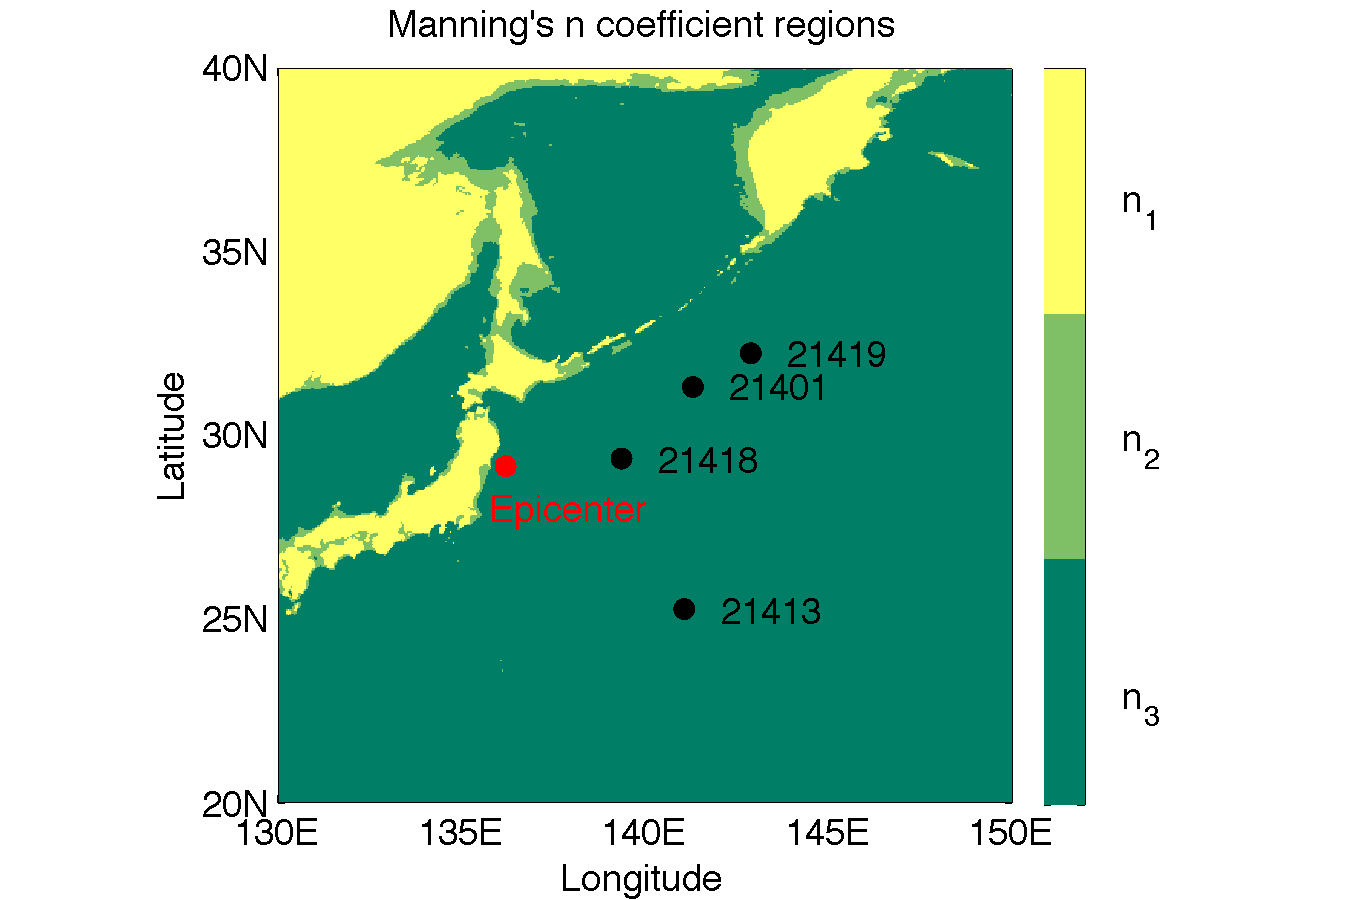
\includegraphics[width=0.6\textwidth]{Figure1.pdf}
\caption{Manning's $n$ coefficients at three regions: $n_1$ on-shore, $n_2$ near shore, $n_3$ deep-water.}
\label{fig:ceofs}
\end{figure}  
%%%%%%%%%%%%%%%%%%%%%%%%%%%%%%%%%%%%%%%%%%%%%%%%%%%%%%%%%%%%%%%%

\begin{figure}[ht]
\centering
\begin{subfigure}[c]{0.45\textwidth}
    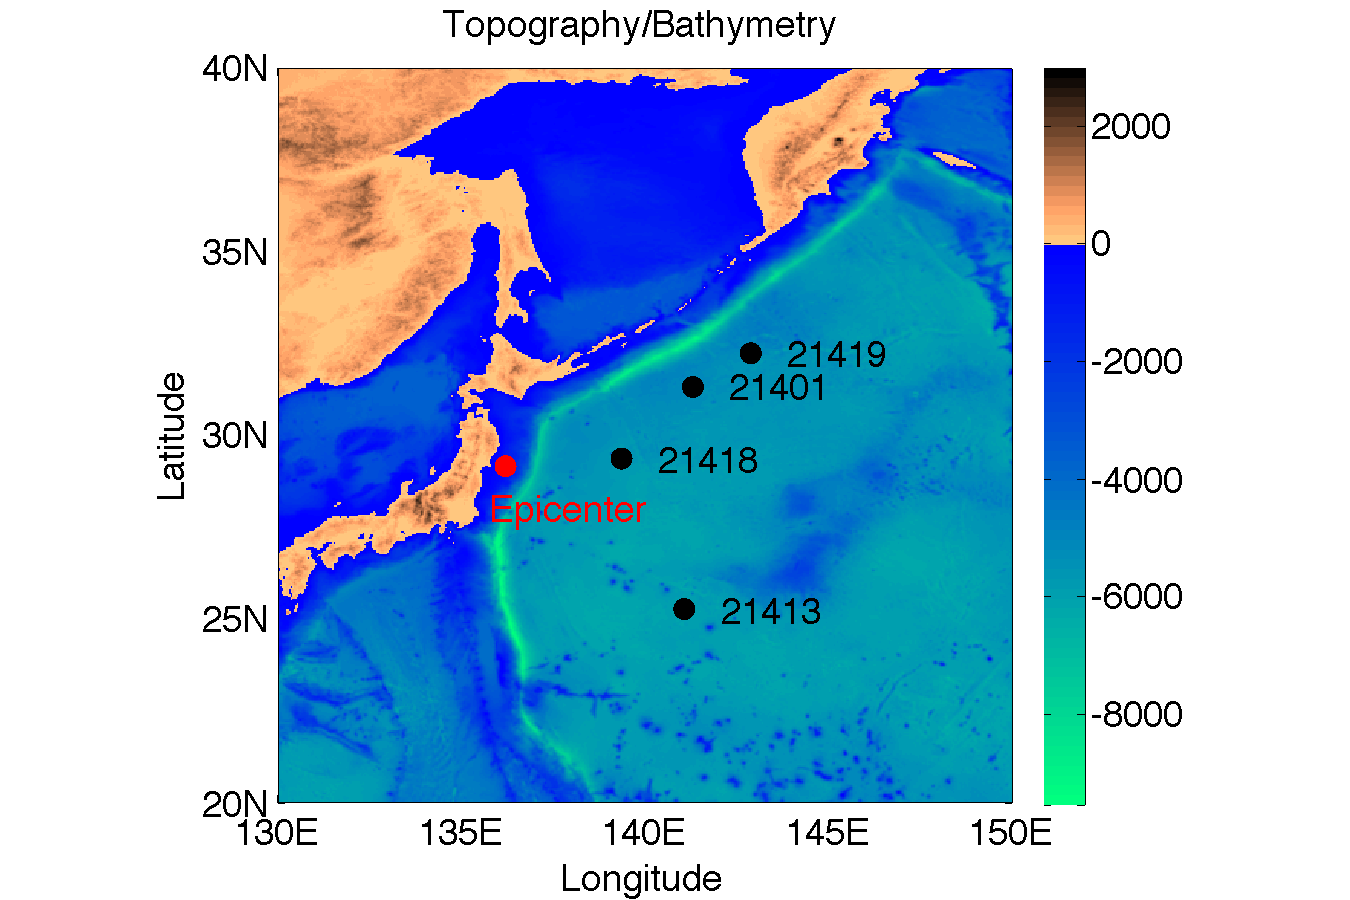
\includegraphics[width=\textwidth]{Figure2a.pdf}
    \caption{} \label{fig:setup_buoy_locations}
\end{subfigure}
\begin{subfigure}[c]{0.45\textwidth}
    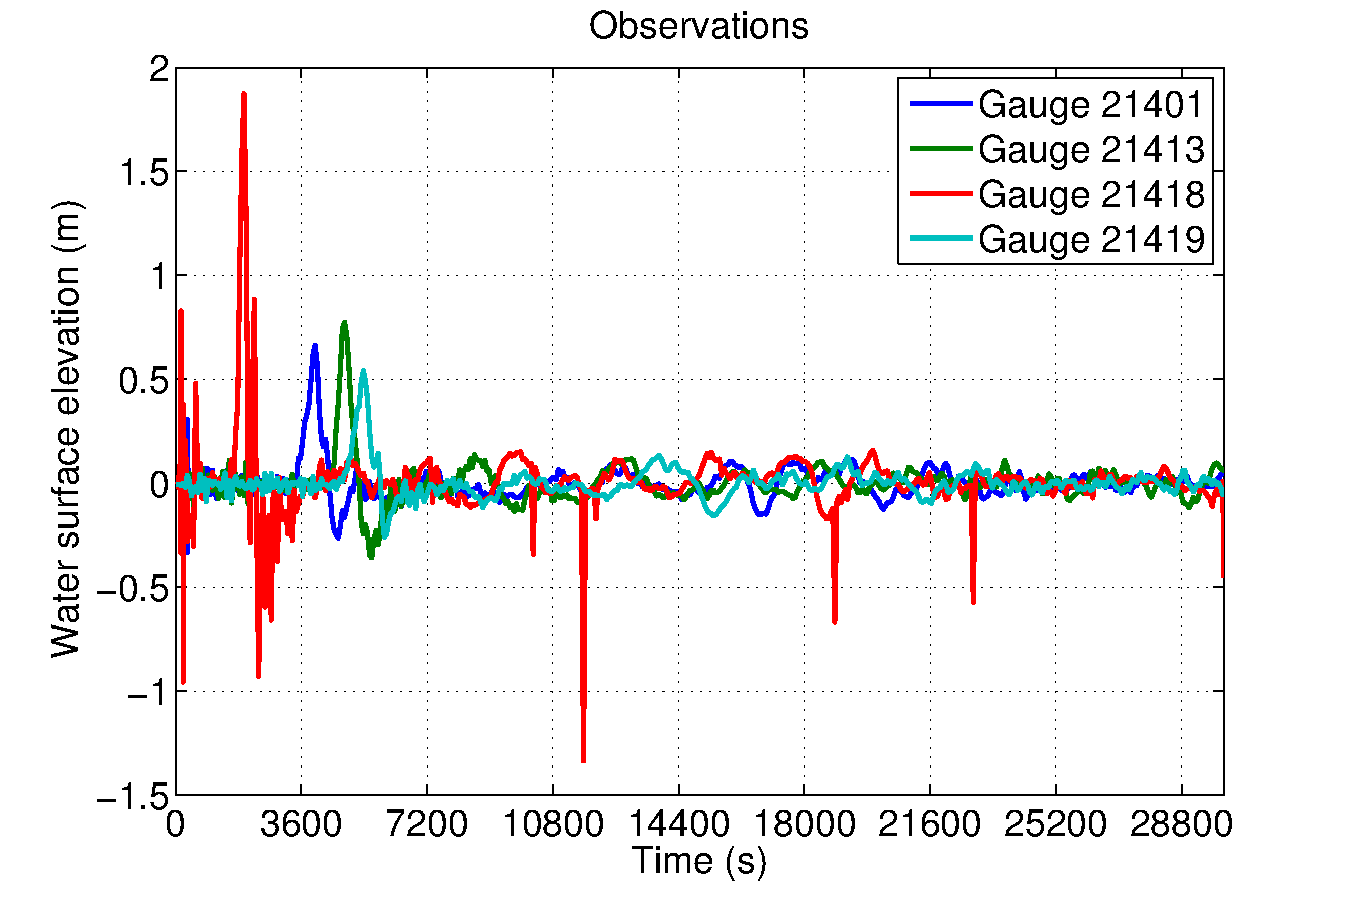
\includegraphics[width=\textwidth]{Figure2b.pdf} 
    \caption{} \label{fig:setup_buoy_data}
\end{subfigure}
\caption{(a) The topography, bathymetry and gauge locations used in the simulation. (b) Observed de-tided water surface height at all the DART buoys used.}
\label{fig:setup}
\end{figure}

%%%%%%%%%%%%%%%%%%%%%%%%%%%%%%%%%%%%%%%%%%%%%%%%%%%%%%%%%%%%%%%%
\begin{figure}[ht]
\centering
\begin{tabular}{clc}        
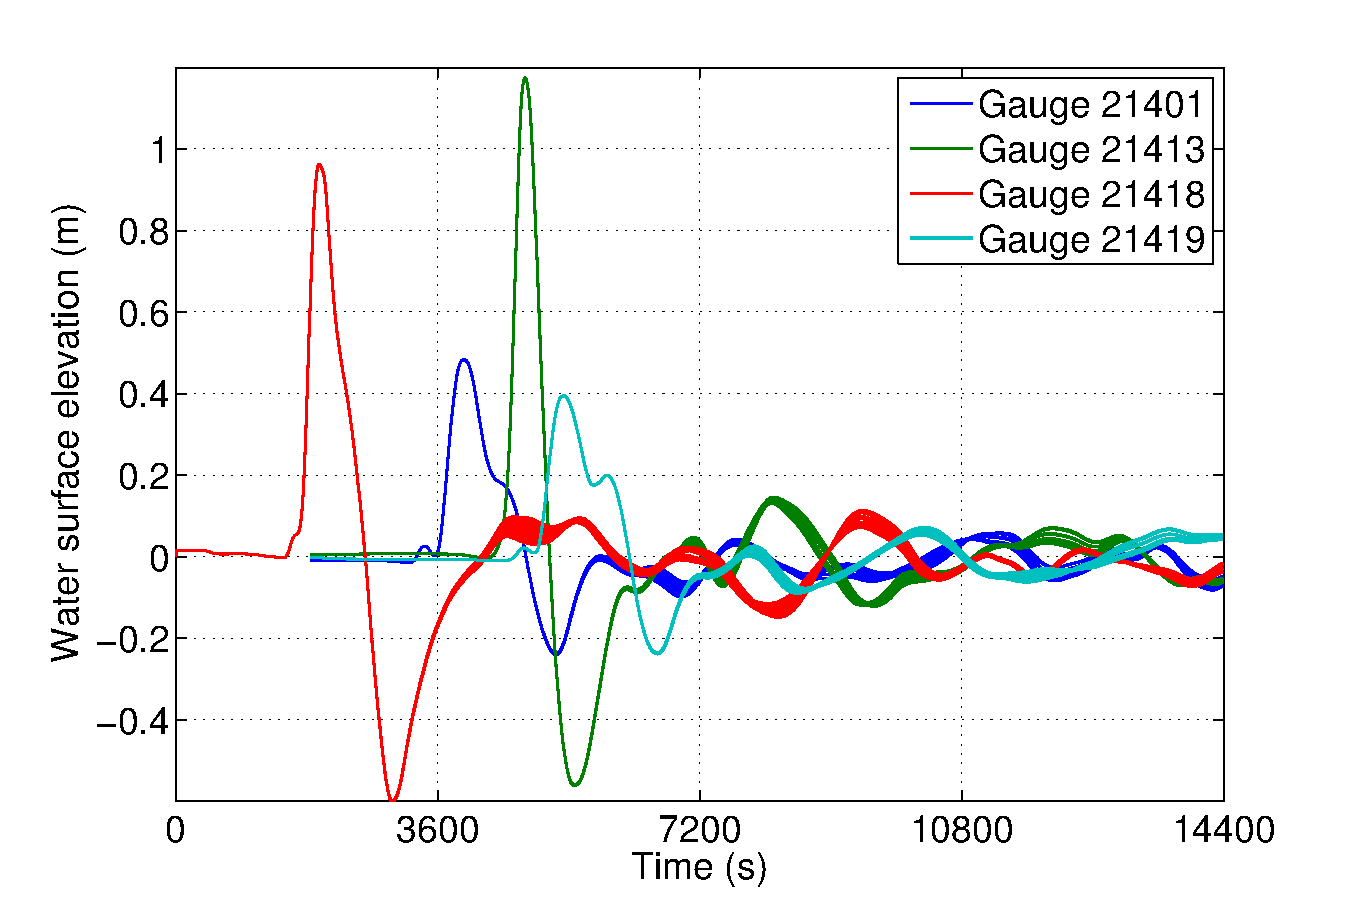
\includegraphics[width=0.6\textwidth]{Figure3.pdf} 
\end{tabular}
\caption{125 \geoclaw realizations at different gauge locations.}
\label{fig:rlzs}
\end{figure}
%%%%%%%%%%%%%%%%%%%%%%%%%%%%%%%%%%%%%%%%%%%%%%%%%%%%%%%%%%%%%%%%

\begin{figure}[ht]
\centering
\begin{tabular}{clc}        
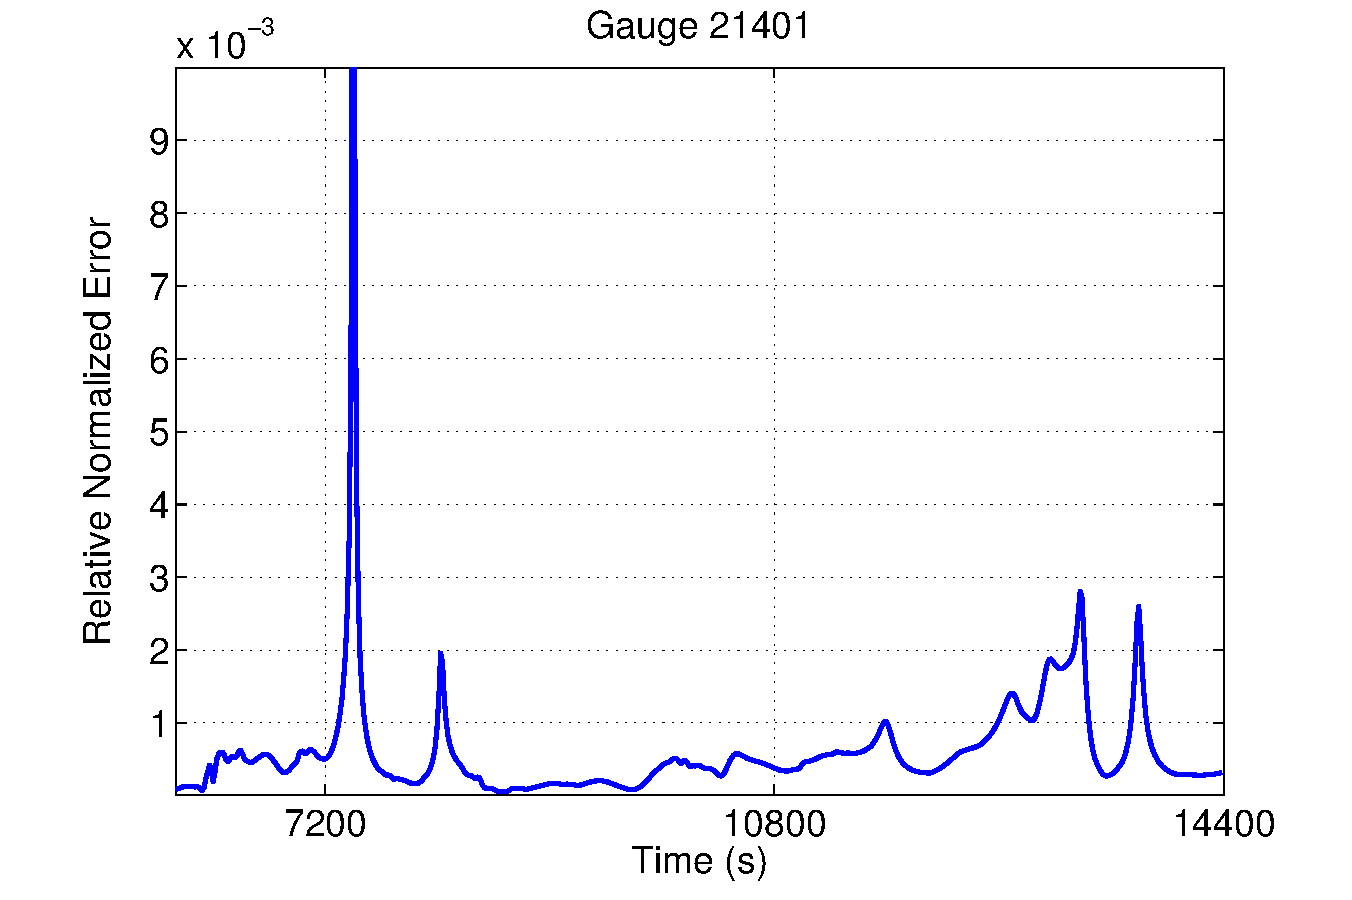
\includegraphics[width=0.5\textwidth]{Figure4a.pdf} &
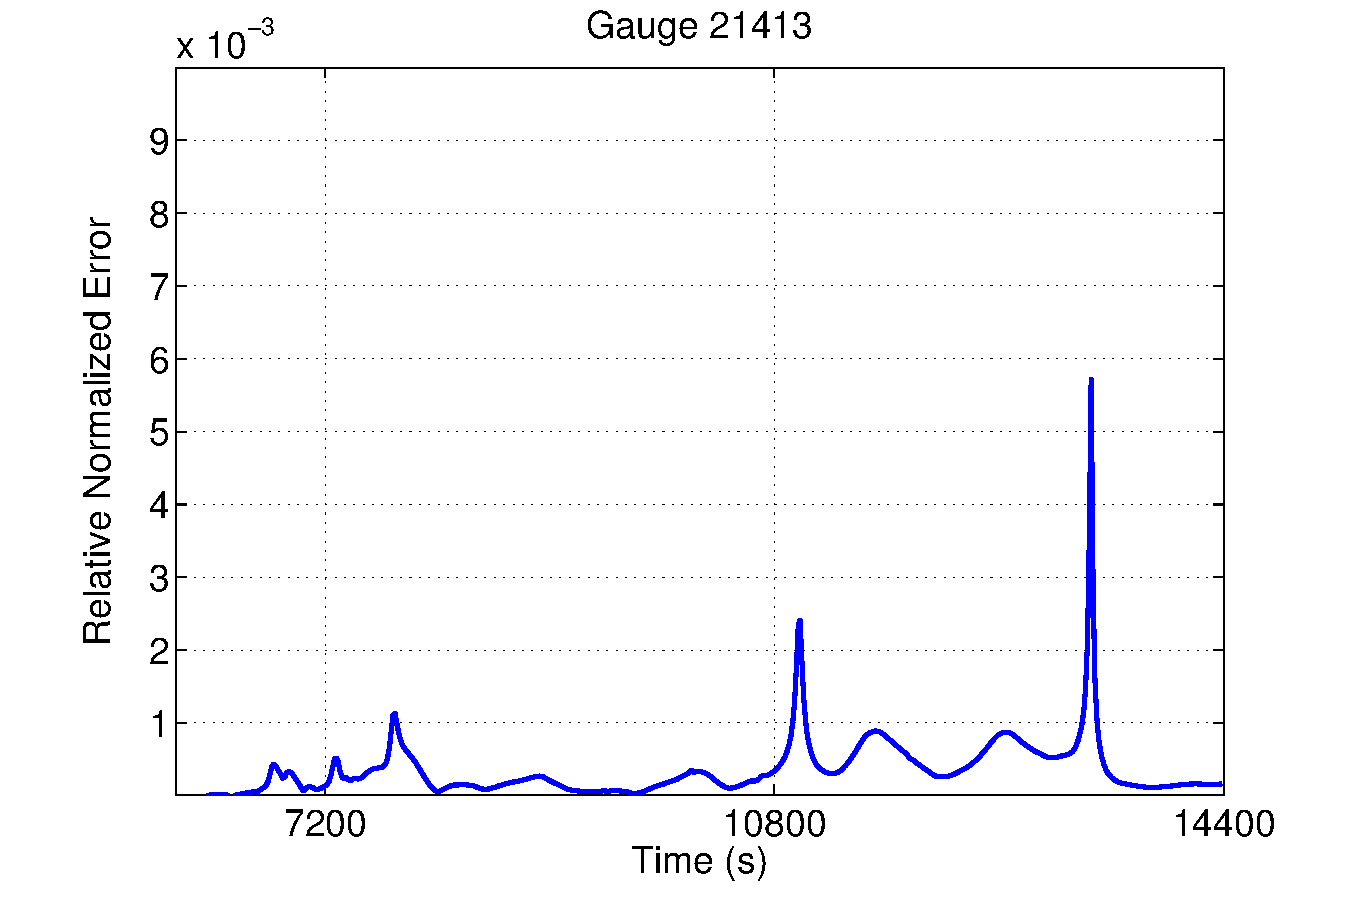
\includegraphics[width=0.5\textwidth]{Figure4b.pdf} \\
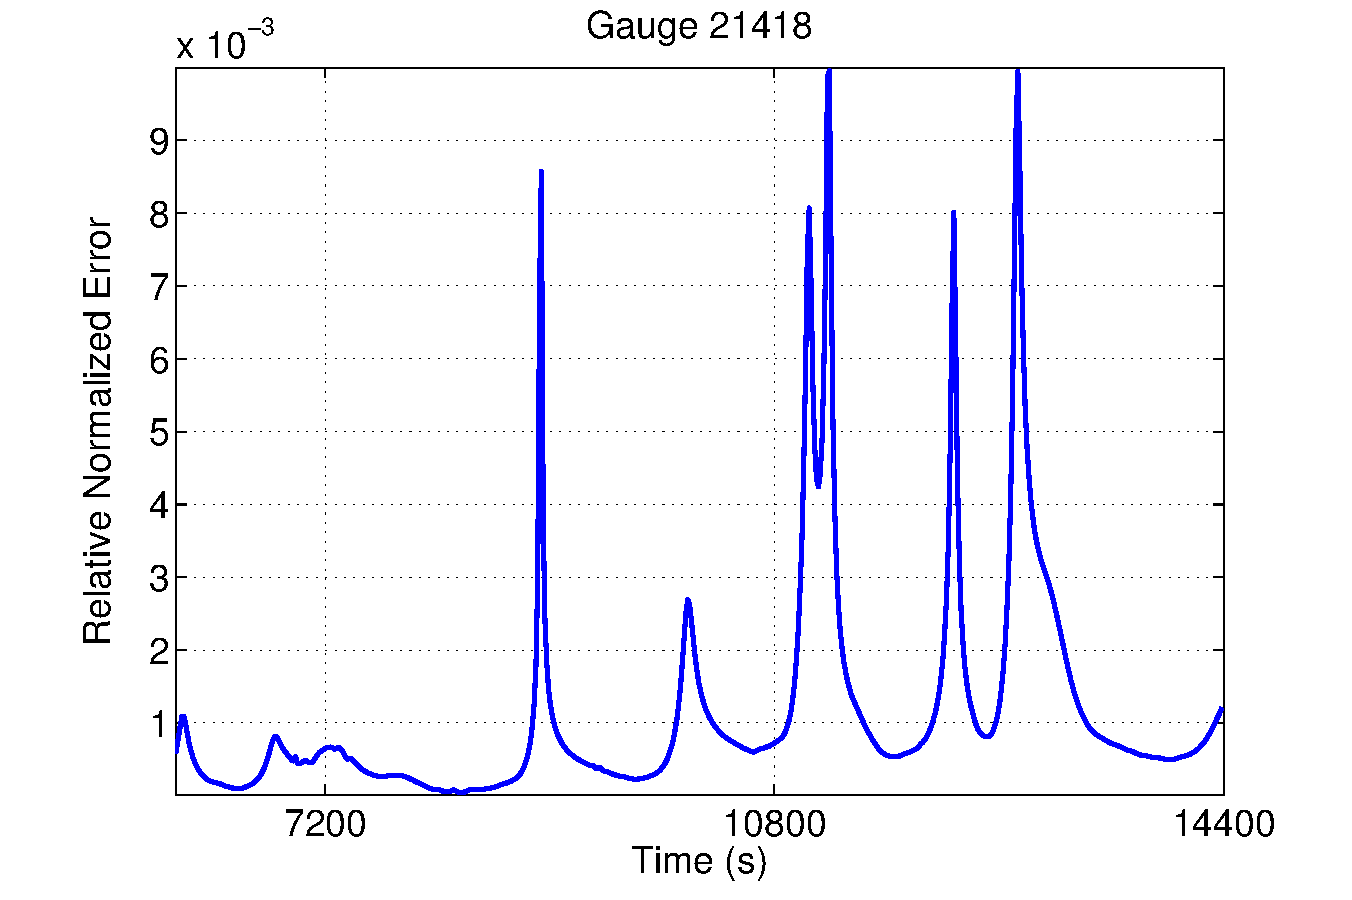
\includegraphics[width=0.5\textwidth]{Figure4c.pdf} &
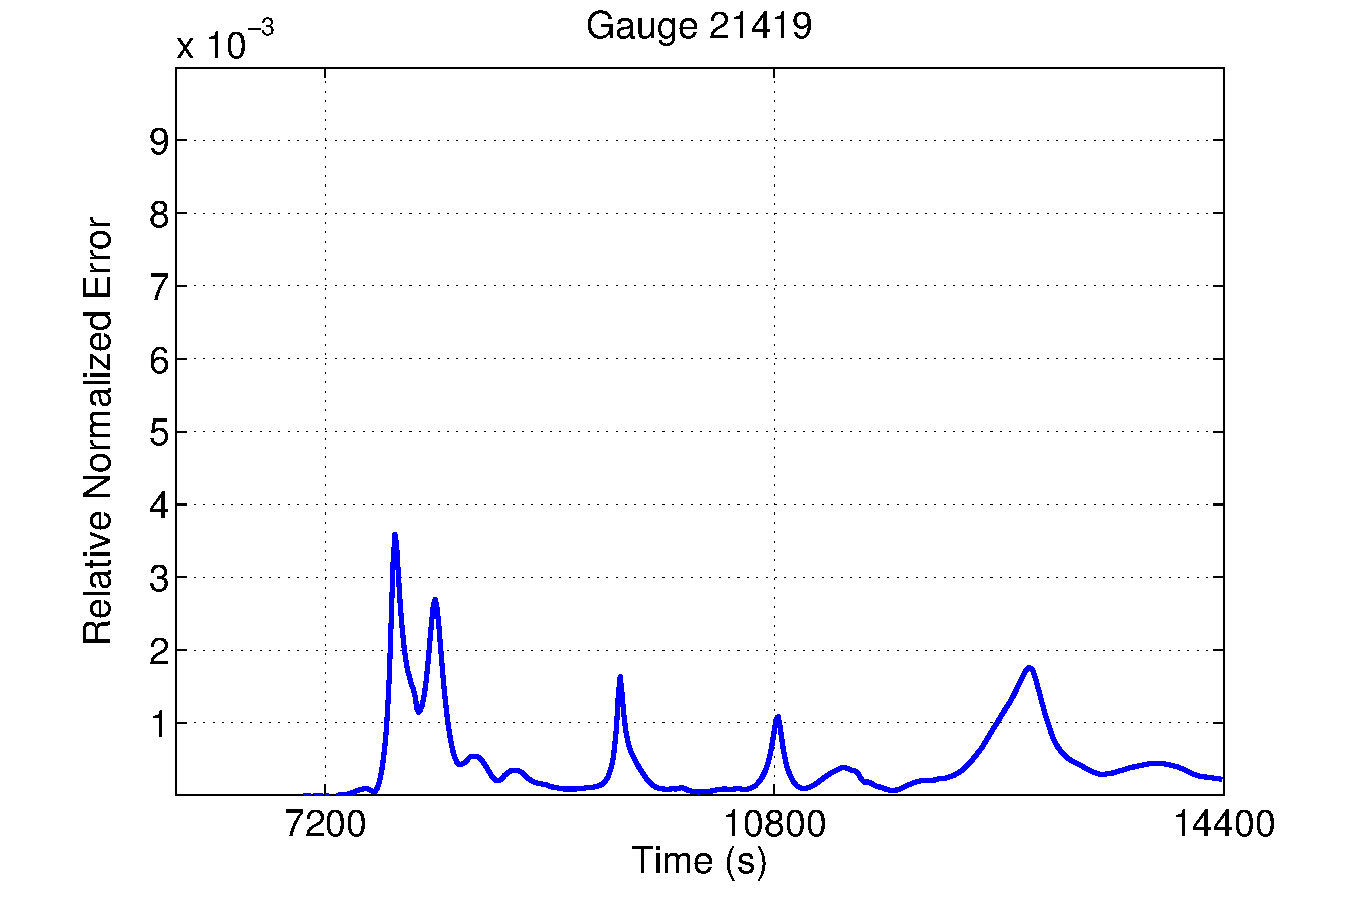
\includegraphics[width=0.5\textwidth]{Figure4d.pdf} 

\end{tabular}
\caption{Relative normalized error between realizations and 
the corresponding PC surrogates at different gauge locations
calculated using Equation~(\ref{eq:error}).}
\label{fig:error}
\end{figure}   
%%%%%%%%%%%%%%%%%%%%%%%%%%%%%%%%%%%%%%%%%%%%%%%%%%%%%%%%%%%%%%%%
\begin{figure}[ht]
\centering

\begin{tabular}{clcl}
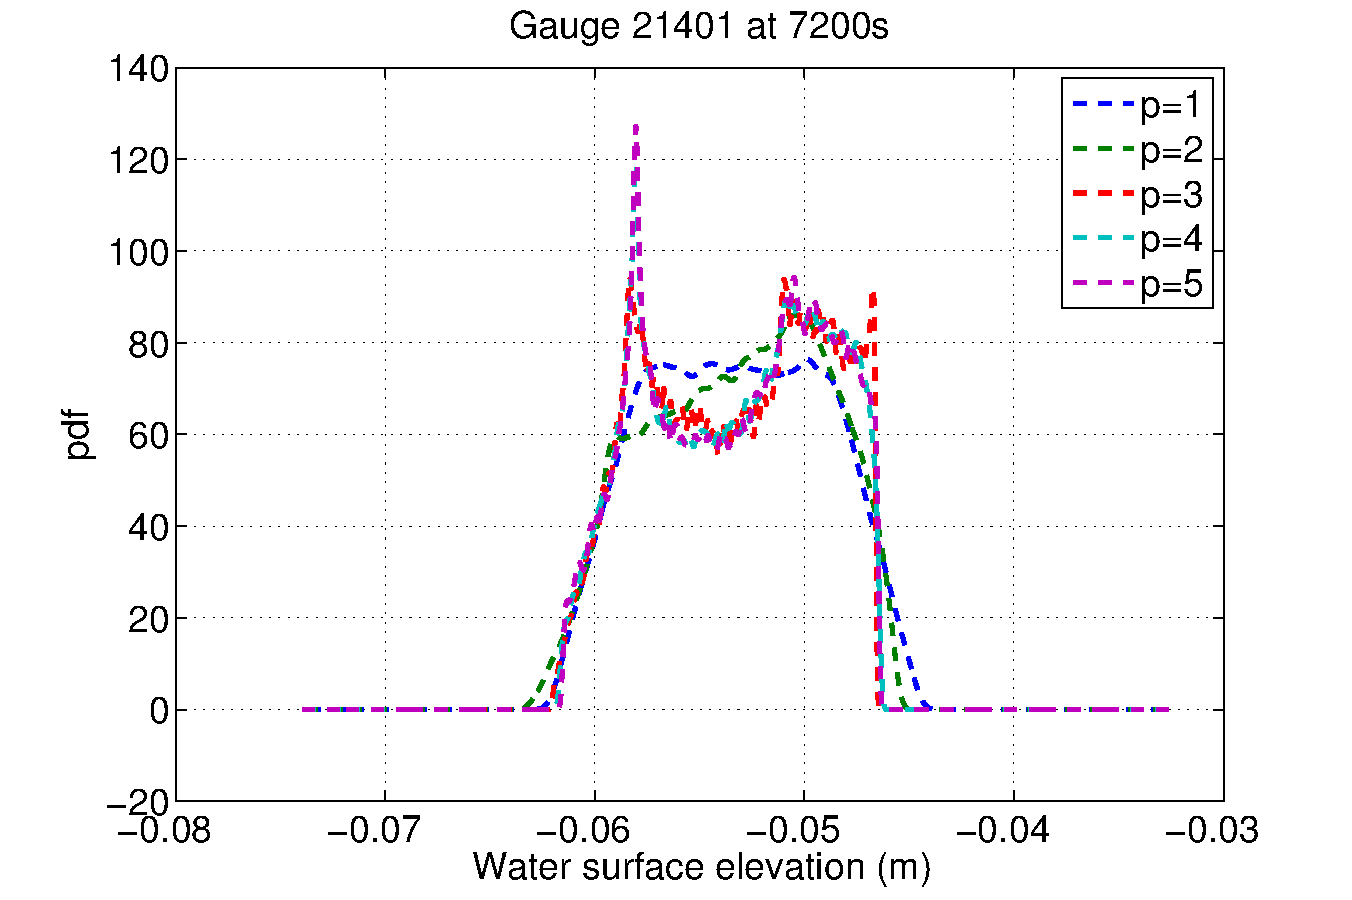
\includegraphics[width=0.5\textwidth]{Figure5a.pdf} &
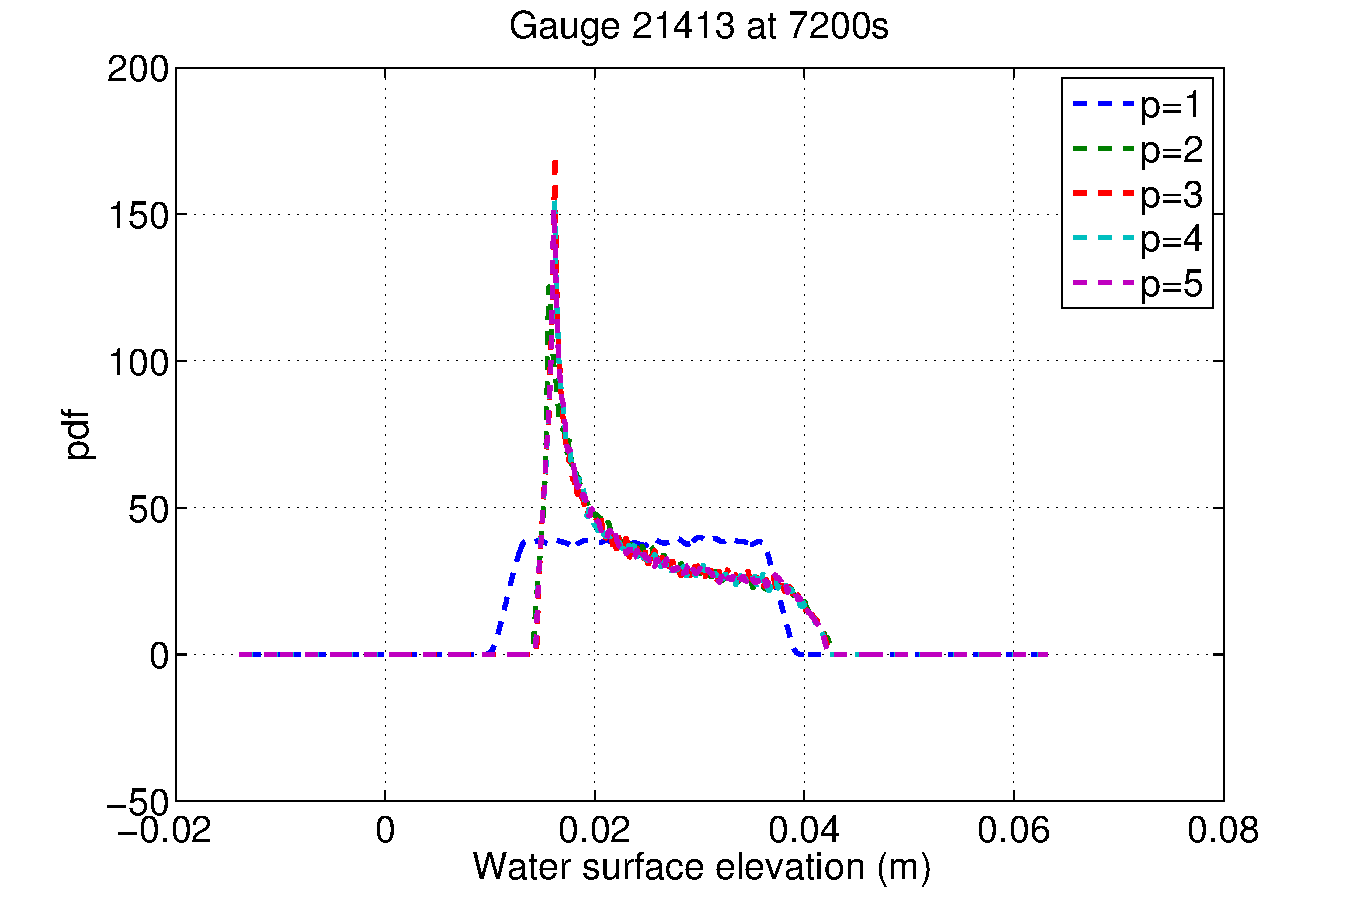
\includegraphics[width=0.5\textwidth]{Figure5b.pdf} \\
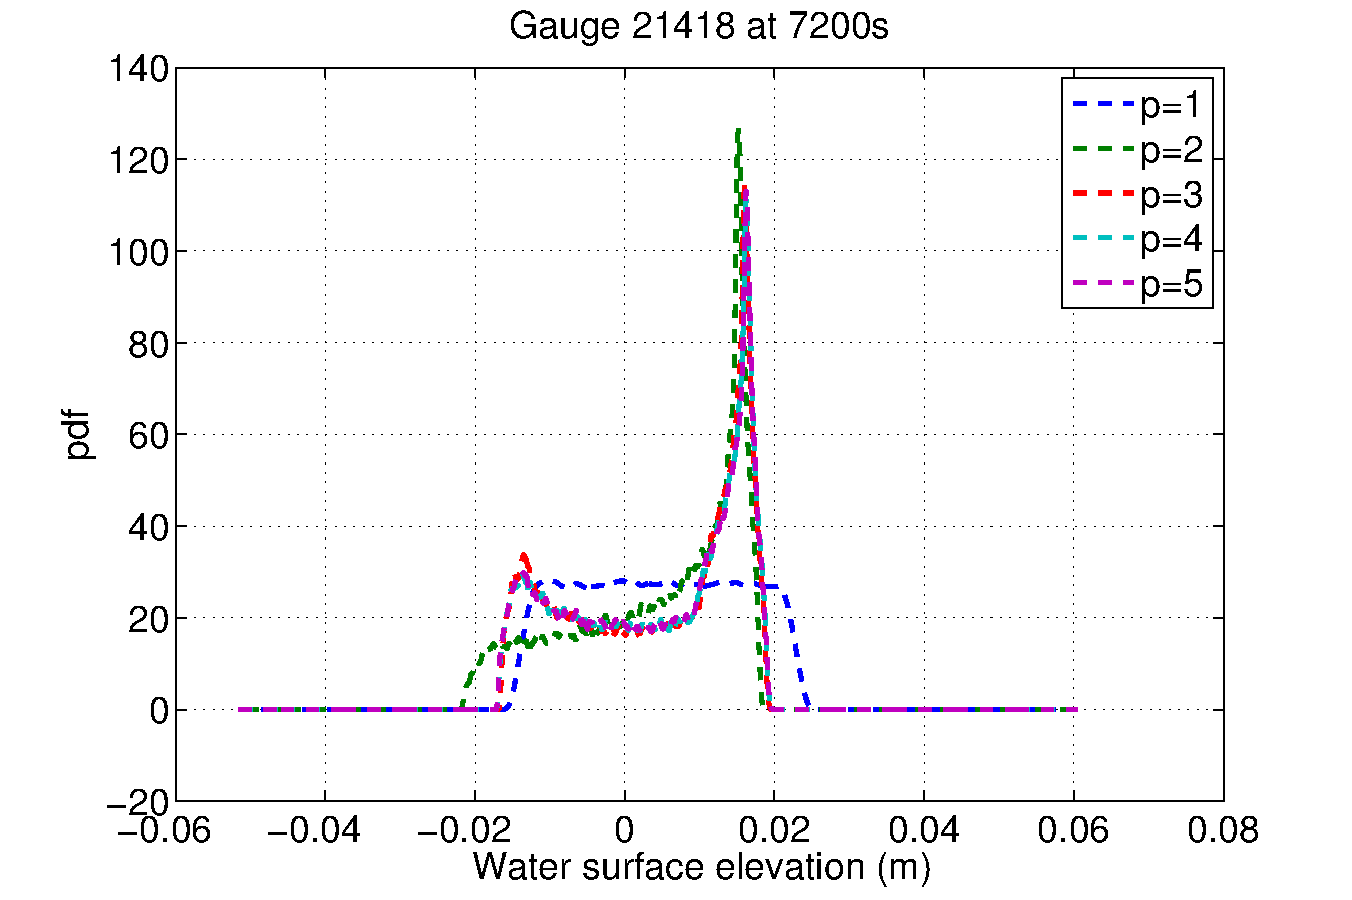
\includegraphics[width=0.5\textwidth]{Figure5c.pdf} &
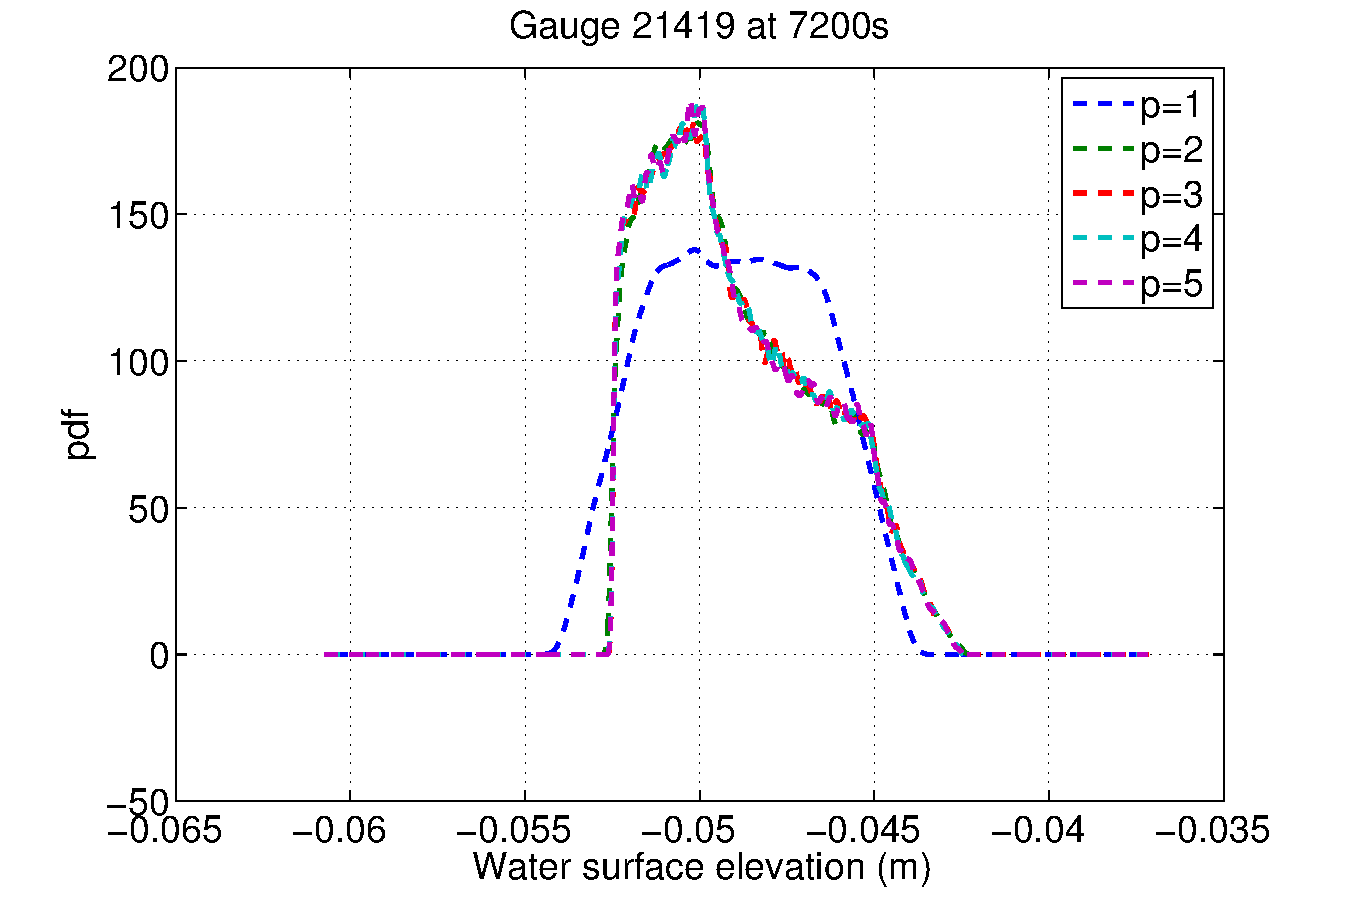
\includegraphics[width=0.5\textwidth]{Figure5d.pdf}
\end{tabular}
\caption{pdf of water surface elevation at the different gauge locations at t = 7200 s.}
\label{fig:pdfs2}
\end{figure}
%%%%%%%%%%%%%%%%%%%%%%%%%%%%%%%%%%%%%%%%%%%%%%%%%%%%%%%%%%%%%%%%
\begin{figure}[ht]
\centering
\begin{tabular}{clc}
        
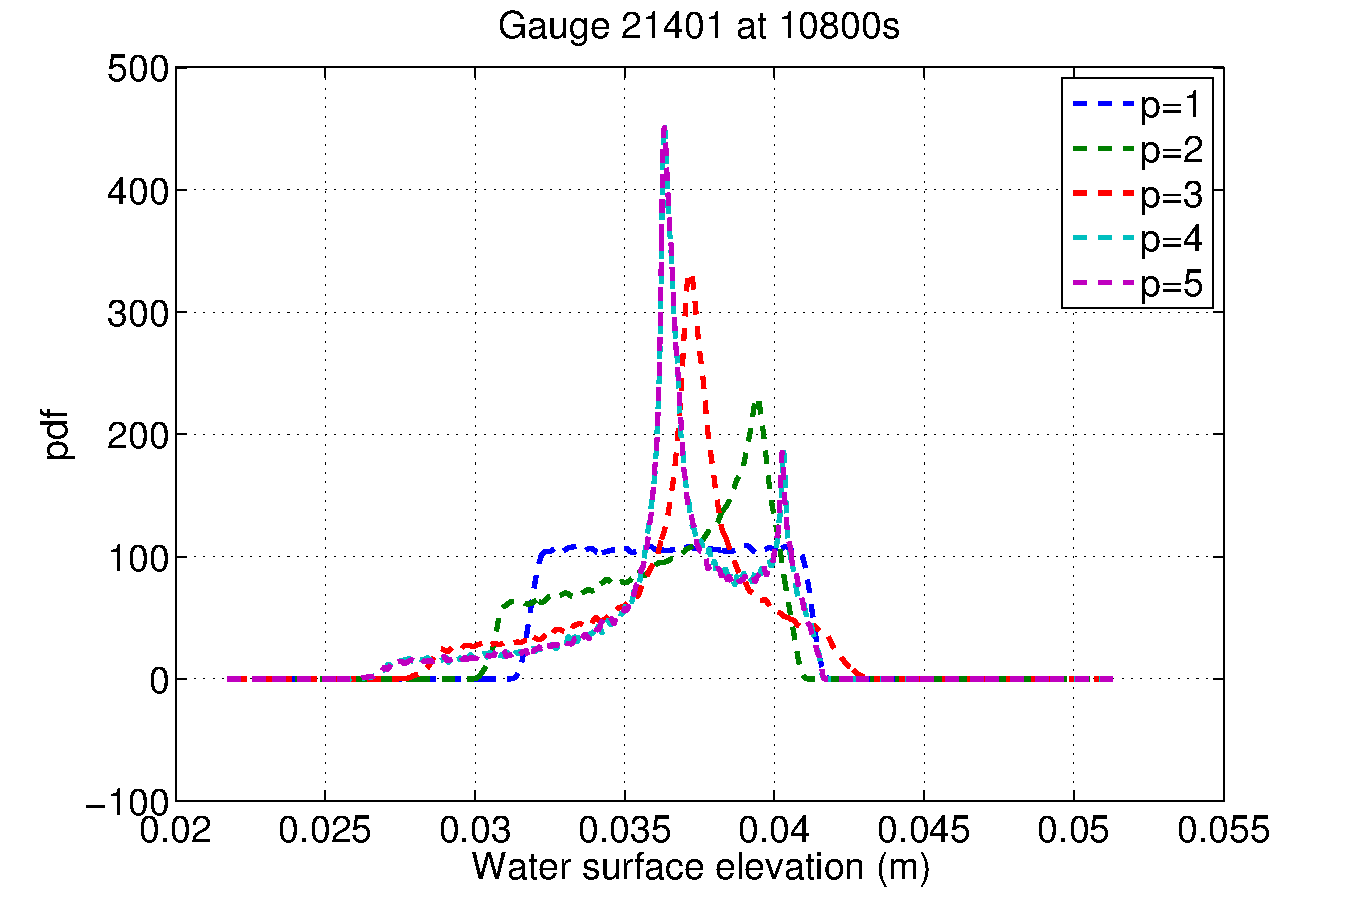
\includegraphics[width=0.5\textwidth]{Figure6a.pdf} &
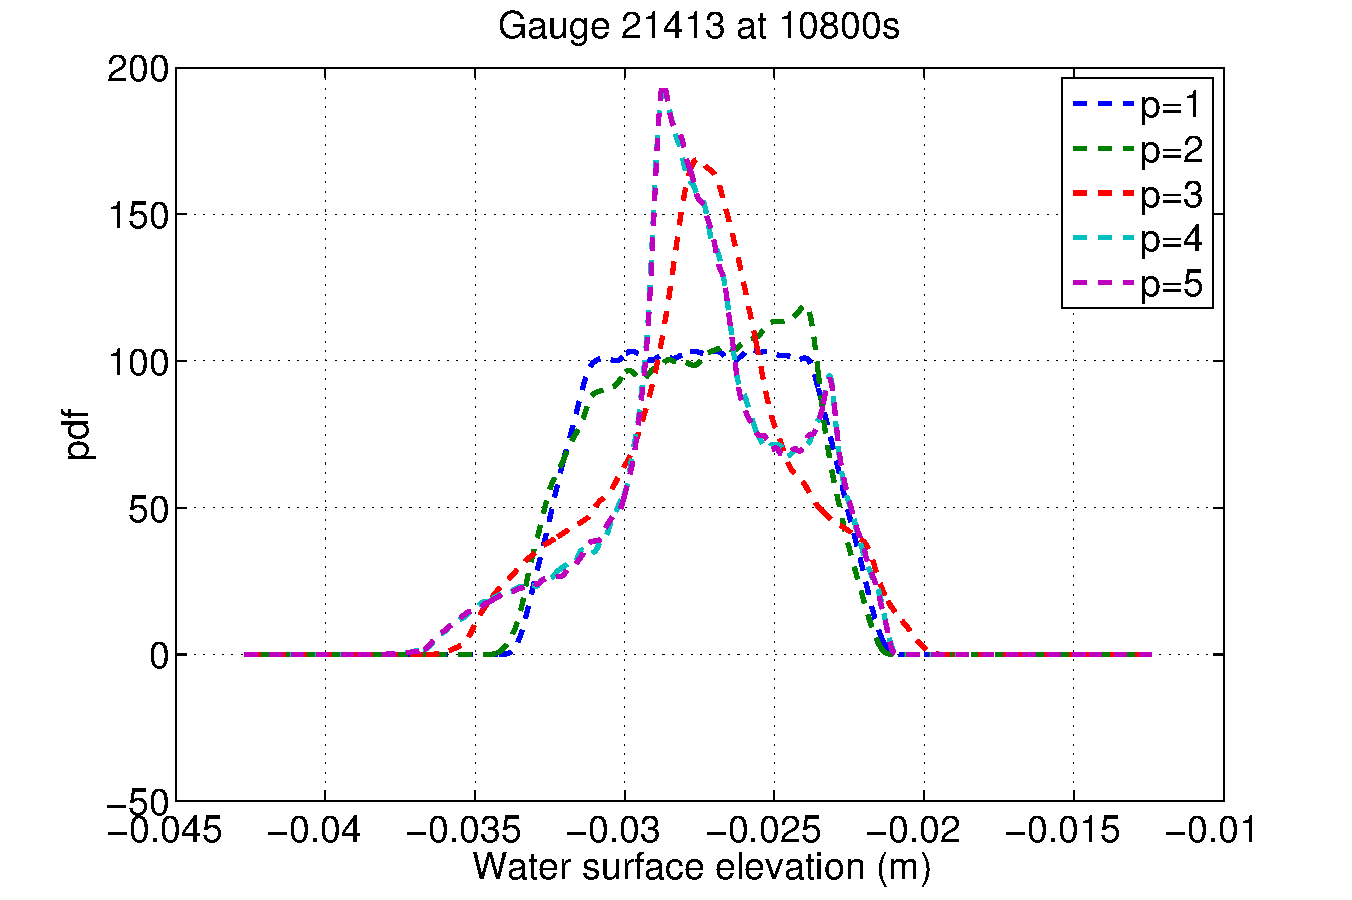
\includegraphics[width=0.5\textwidth]{Figure6b.pdf} \\
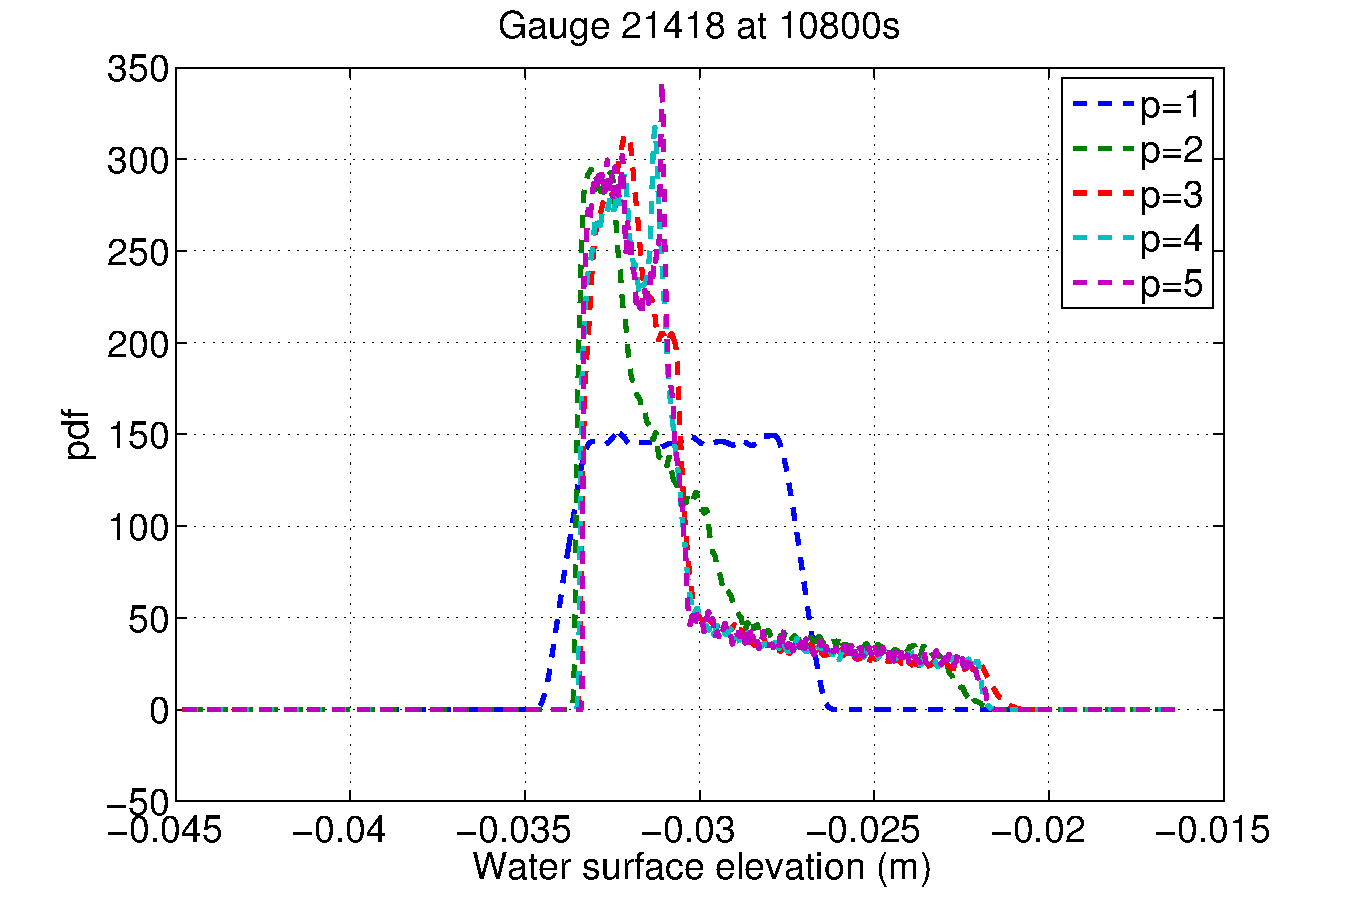
\includegraphics[width=0.5\textwidth]{Figure6c.pdf} &
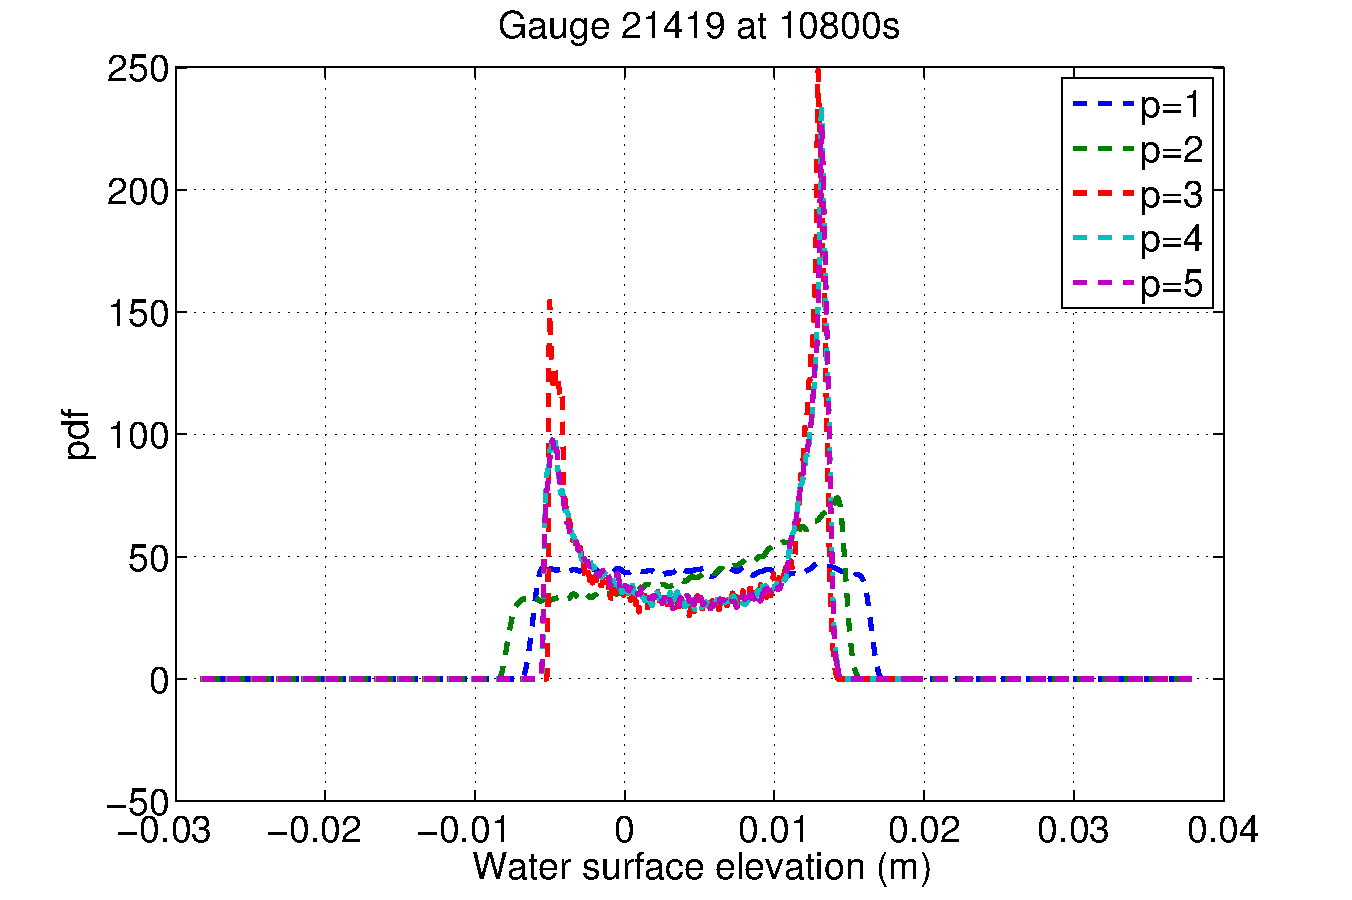
\includegraphics[width=0.5\textwidth]{Figure6d.pdf}
\end{tabular}
\caption{pdf of water surface elevation at the different gauge locations at t = 10800 s.}
\label{fig:pdfs3}
\end{figure}
%%%%%%%%%%%%%%%%%%%%%%%%%%%%%%%%%%%%%%%%%%%%%%%%%%%%%%%%%%%%%%%%
\begin{figure}[ht]
\begin{tabular}{clc}
        
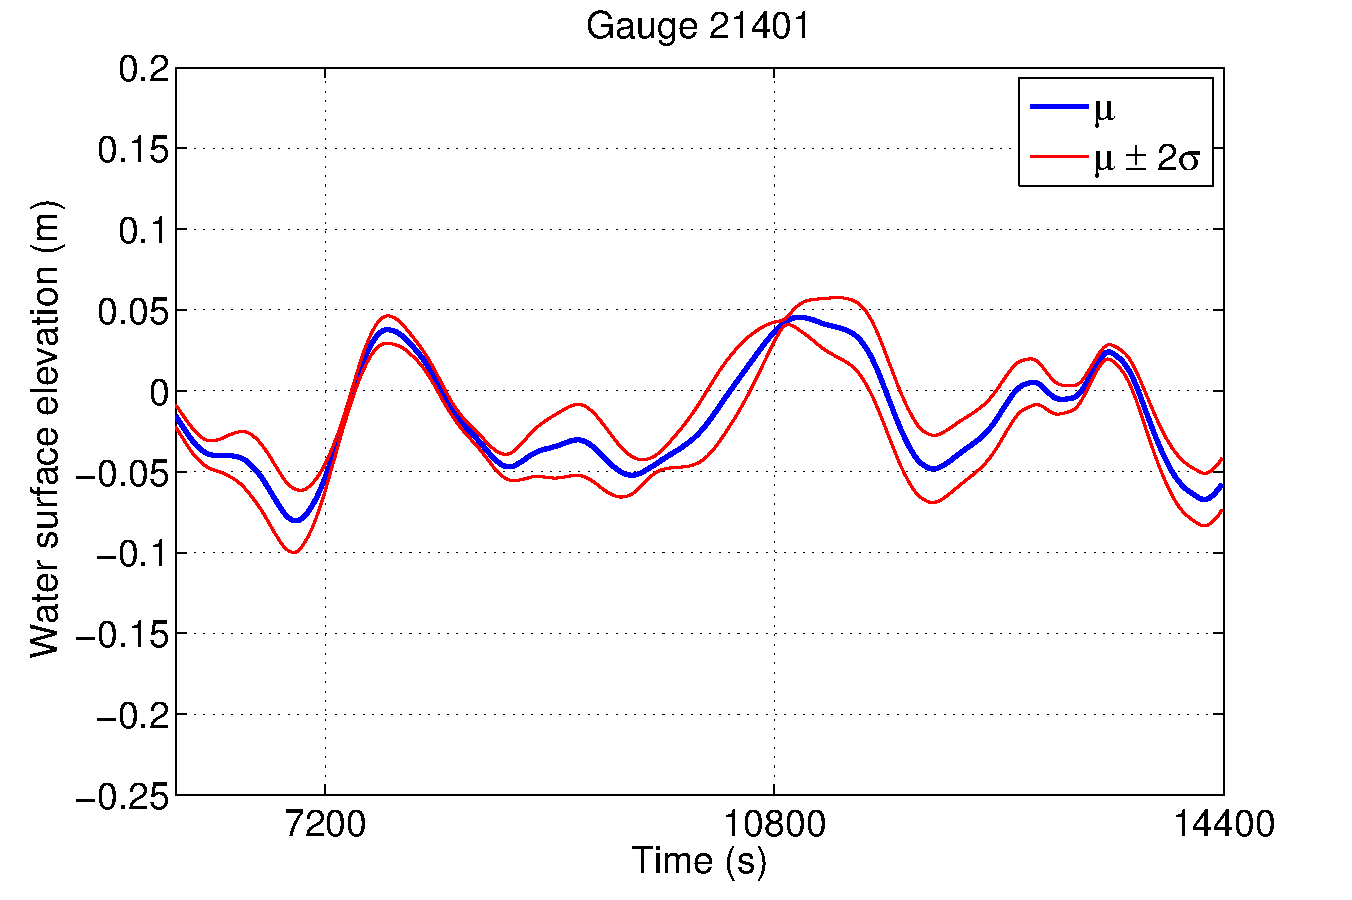
\includegraphics[width=0.475\textwidth]{Figure7a.pdf} &
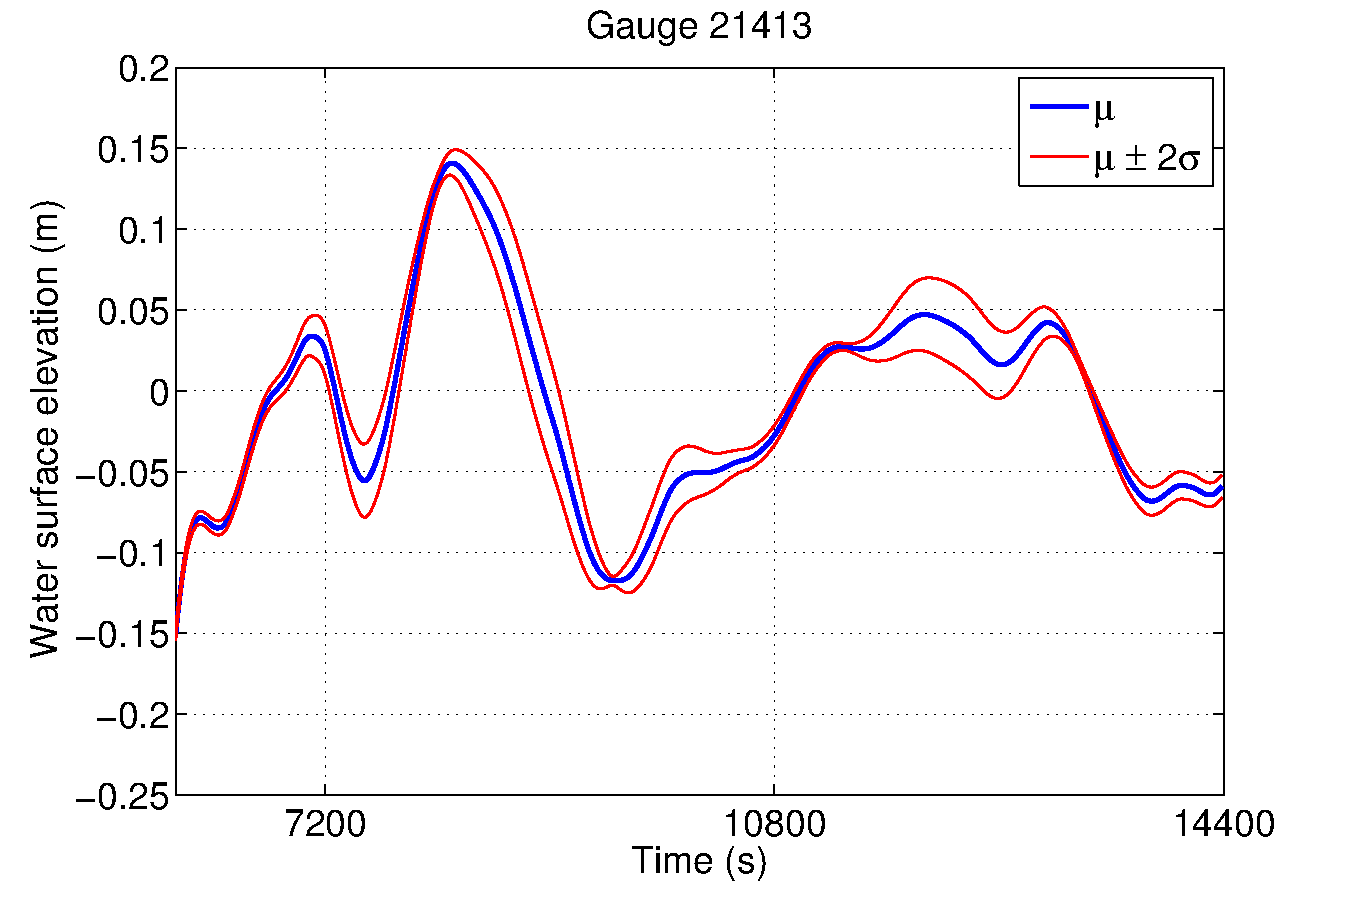
\includegraphics[width=0.475\textwidth]{Figure7b.pdf} \\
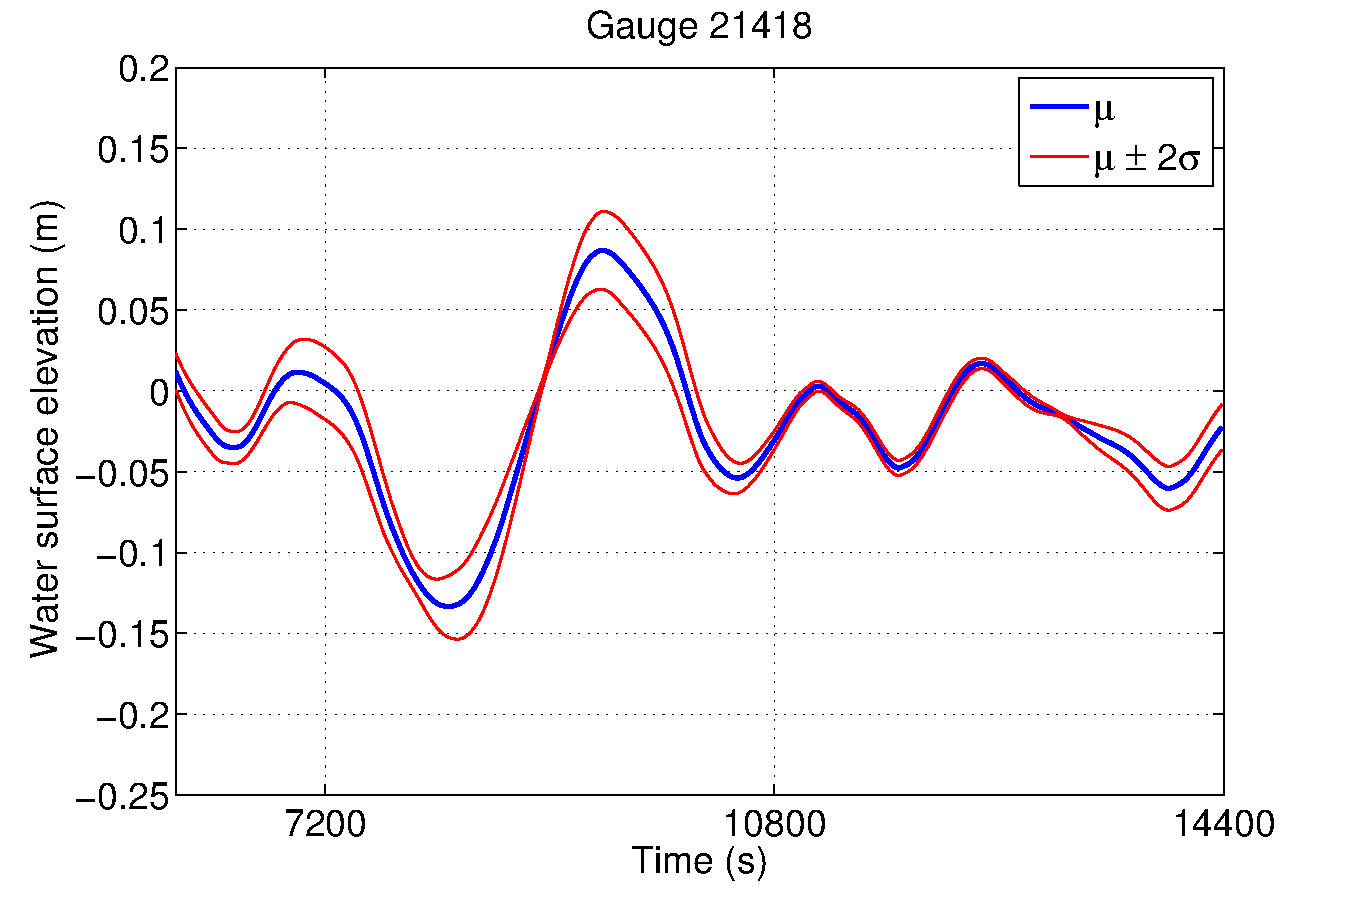
\includegraphics[width=0.475\textwidth]{Figure7c.pdf} &
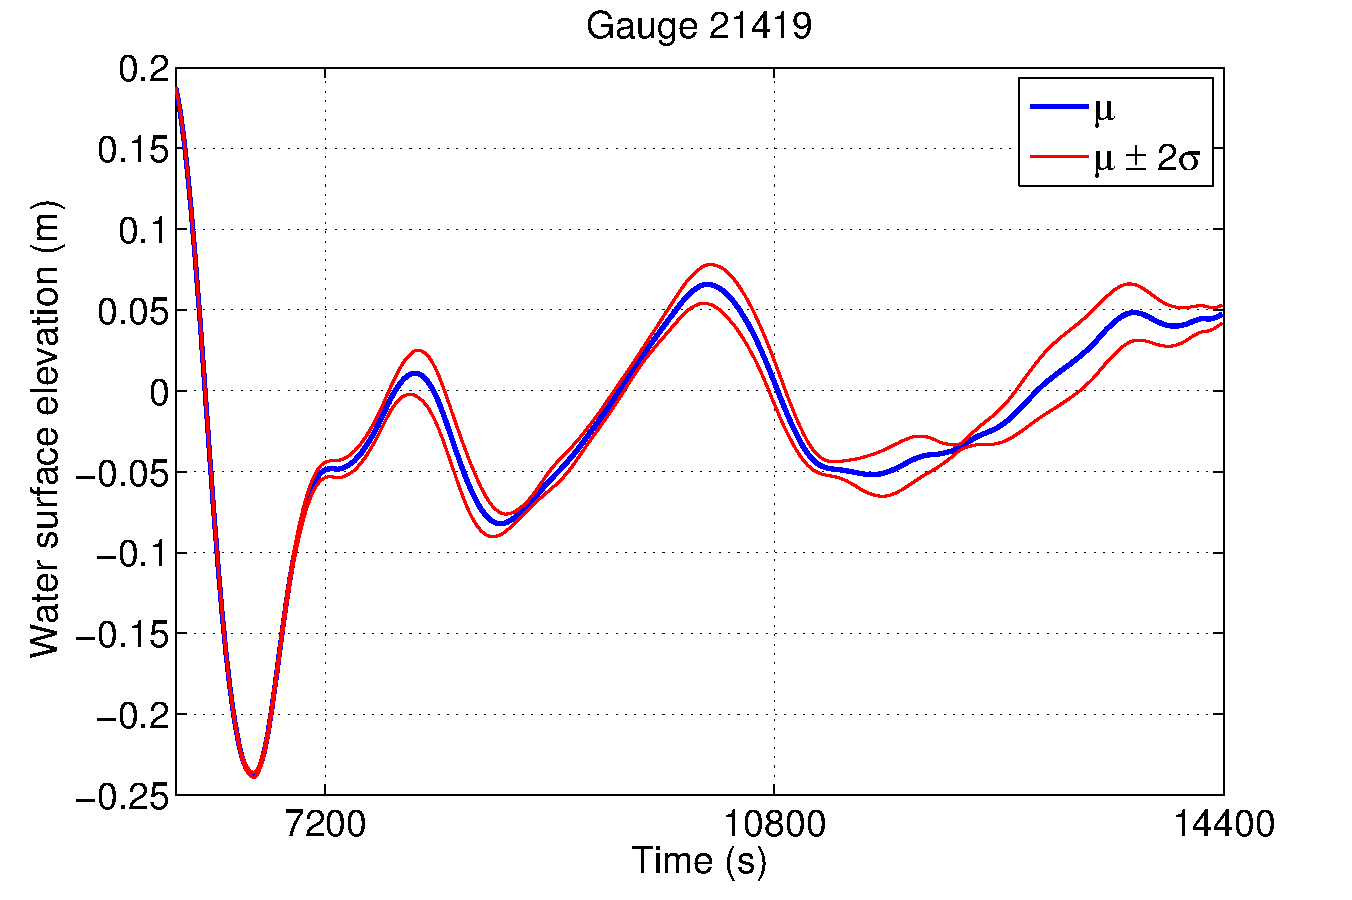
\includegraphics[width=0.475\textwidth]{Figure7d.pdf}
\end{tabular}
\caption{Evolution of PC mean water surface elevation at different gauge locations.}
\label{fig:ave}
\end{figure}
%%%%%%%%%%%%%%%%%%%%%%%%%%%%%%%%%%%%%%%%%%%%%%%%%%%%%%%%%%%%%%%%
\begin{figure}[ht]
\begin{tabular}{clc}
%        
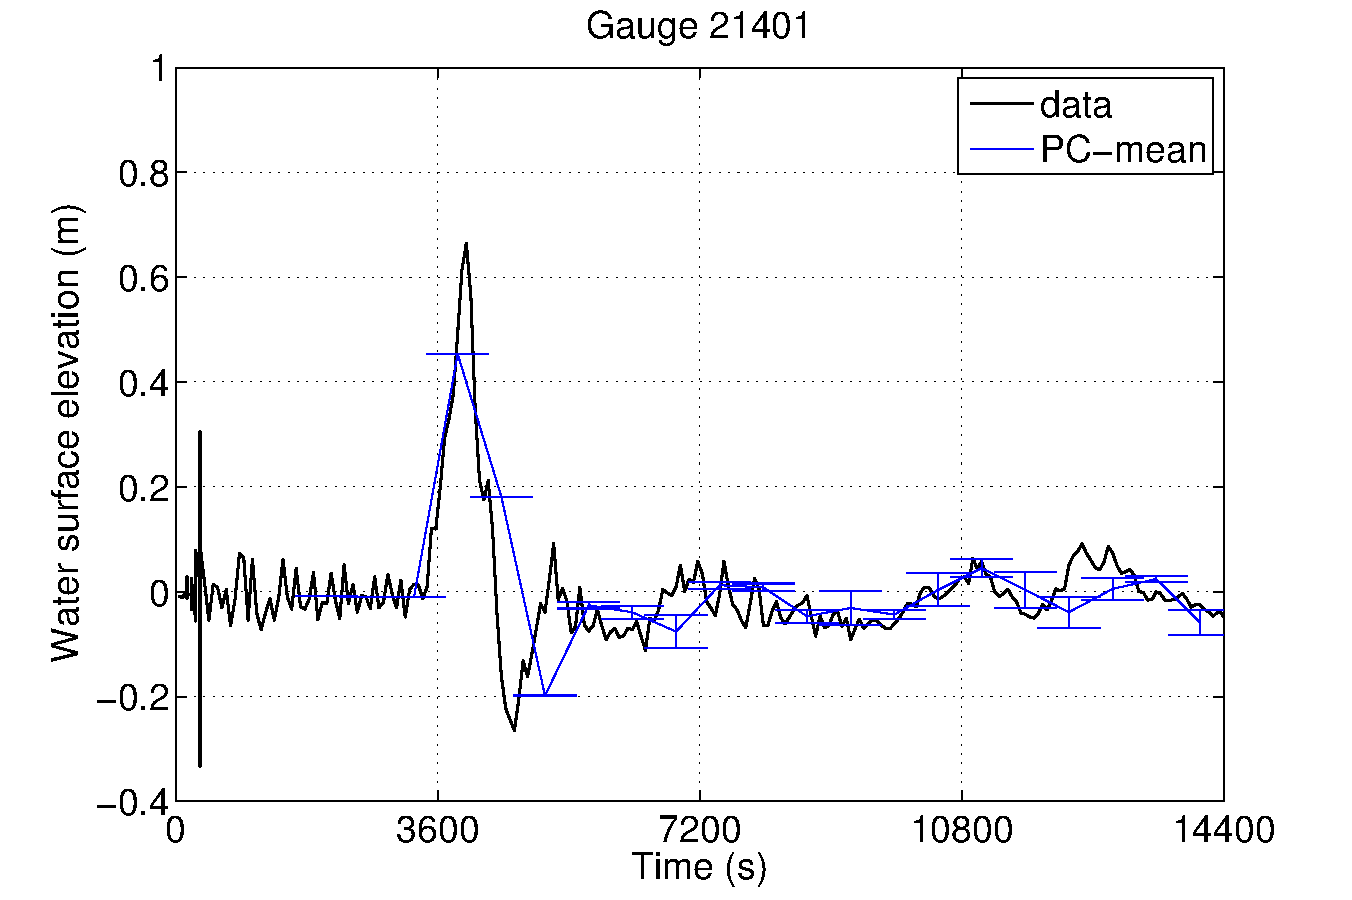
\includegraphics[width=0.475\textwidth]{Figure8a.pdf} &
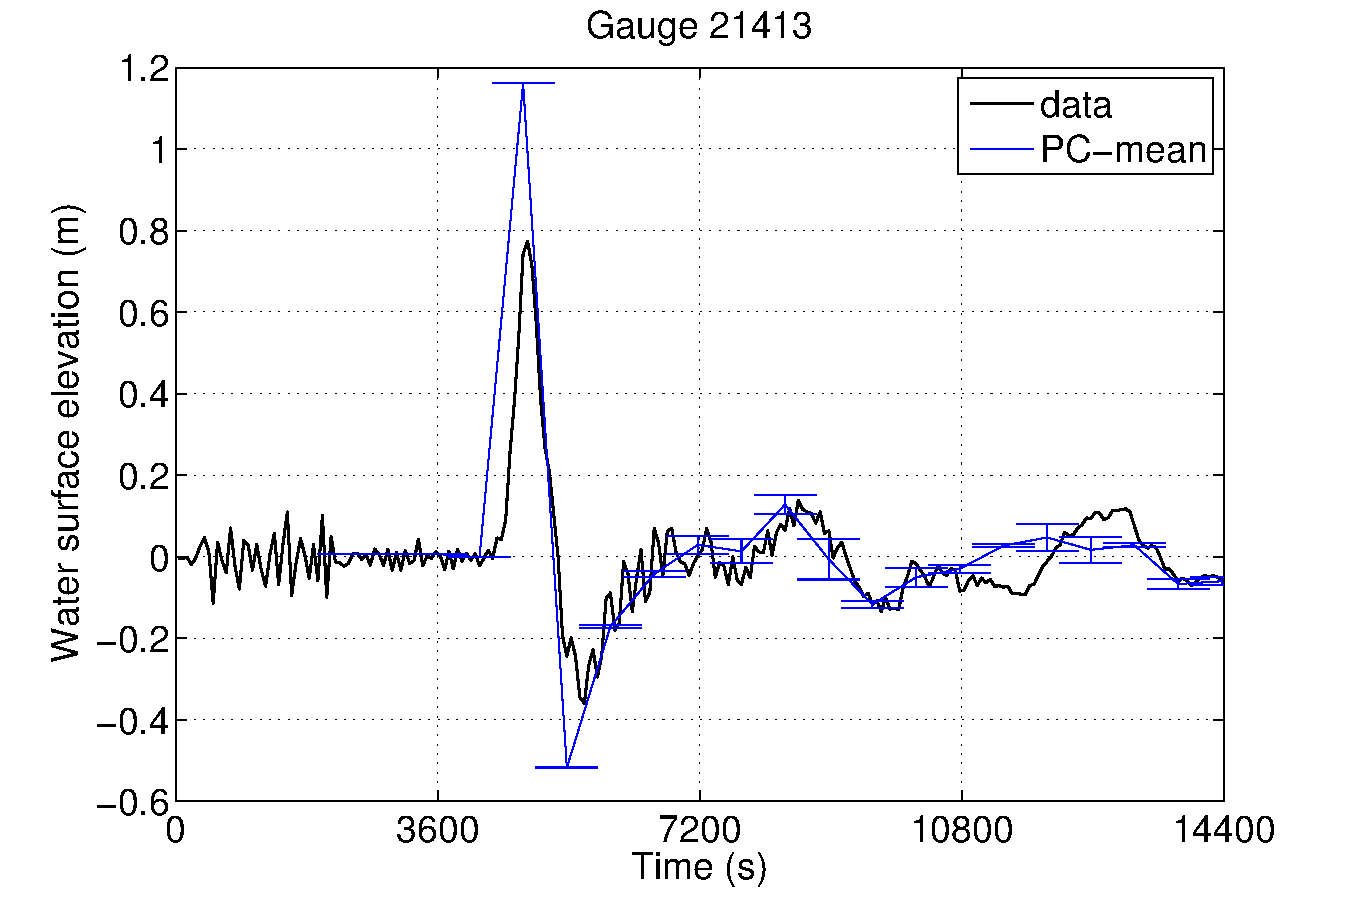
\includegraphics[width=0.475\textwidth]{Figure8b.pdf} \\
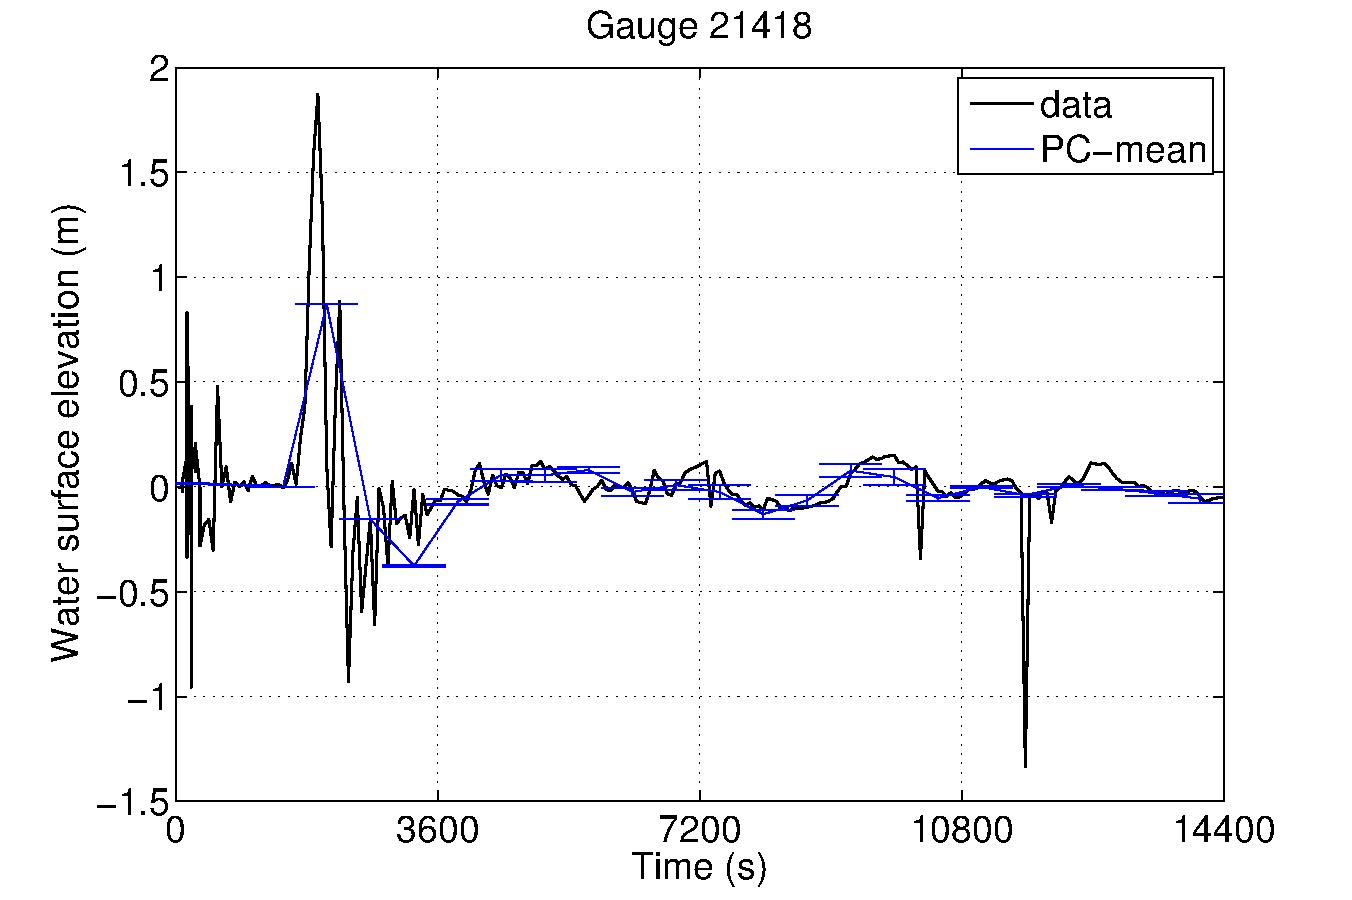
\includegraphics[width=0.475\textwidth]{Figure8c.pdf} &
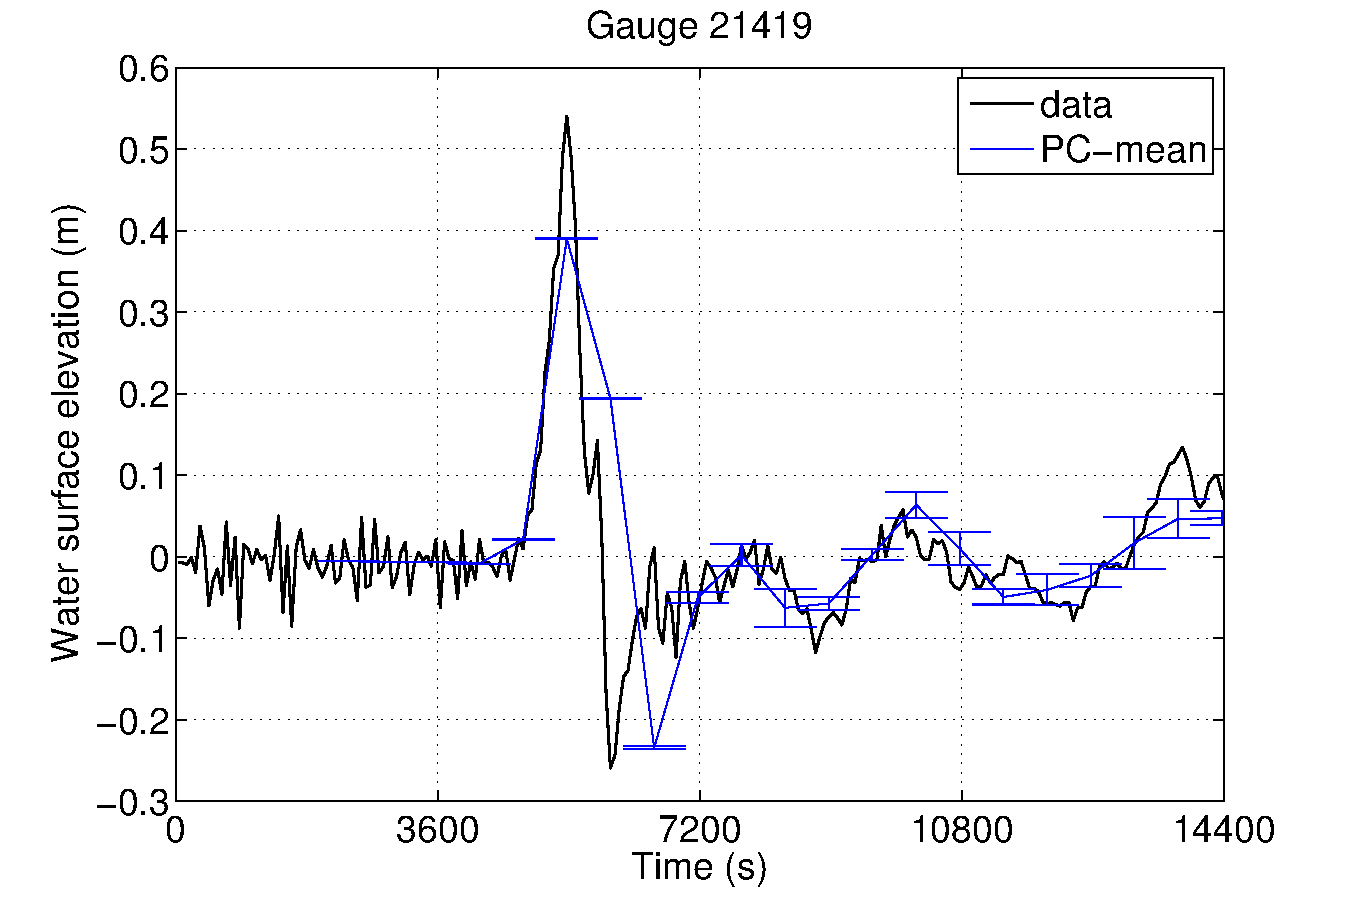
\includegraphics[width=0.475\textwidth]{Figure8d.pdf}
\end{tabular}
\caption{Comparison of PC mean 
and observed data of water surface elevation with time at the four gauges.}
\label{fig:compare}
\end{figure}  
%%%%%%%%%%%%%%%%%%%%%%%%%%%%%%%%%%%%%%%%%%%%%%%%%%%%%%%%%%%%%%%%
\begin{figure}[ht]
        \begin{tabular}{ccc}
\hspace*{-55pt}
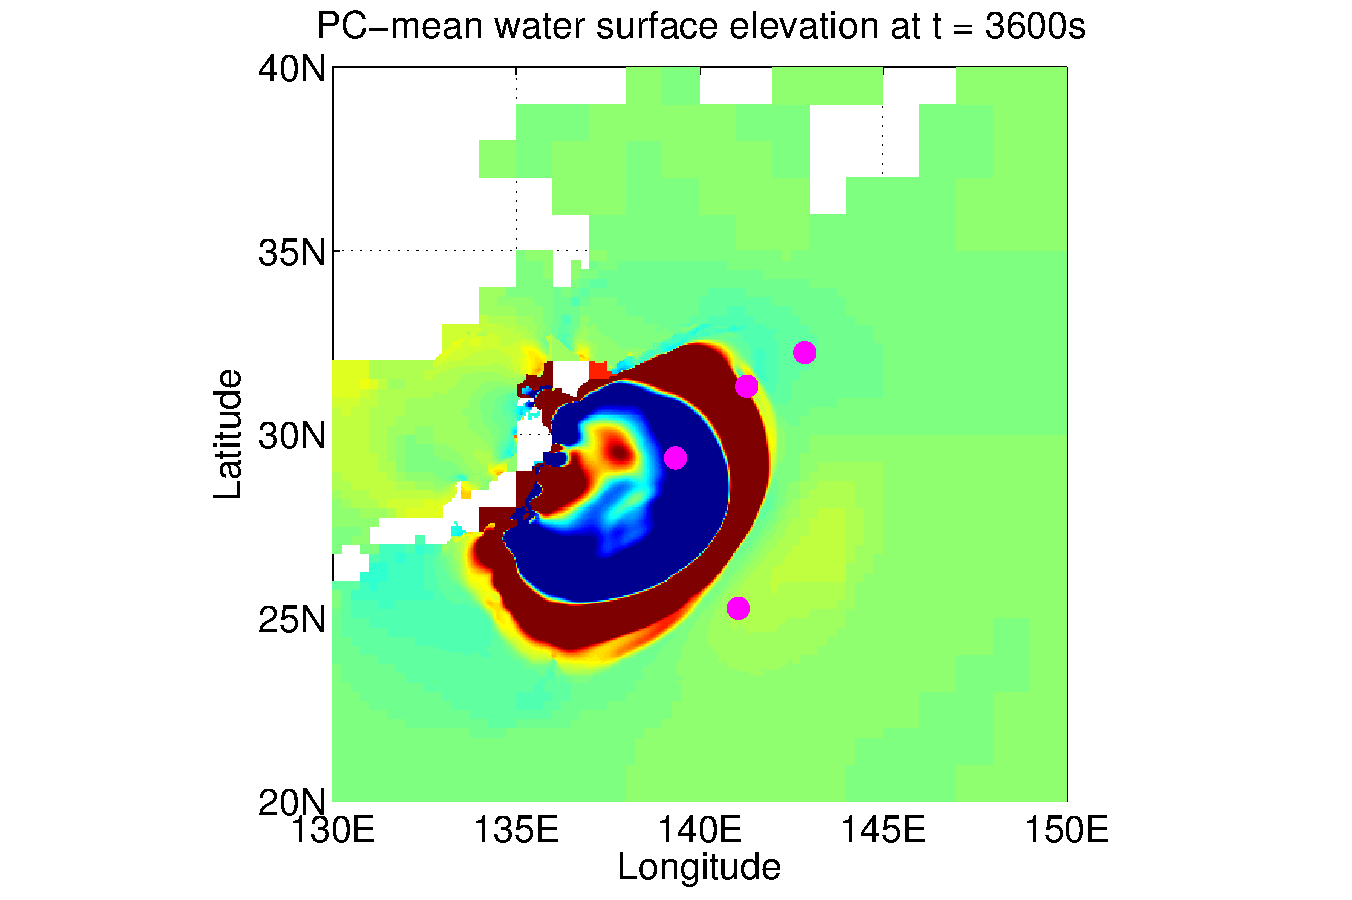
\includegraphics[width=0.45\textwidth]{Figure9a.pdf} &
\hspace*{-45pt}
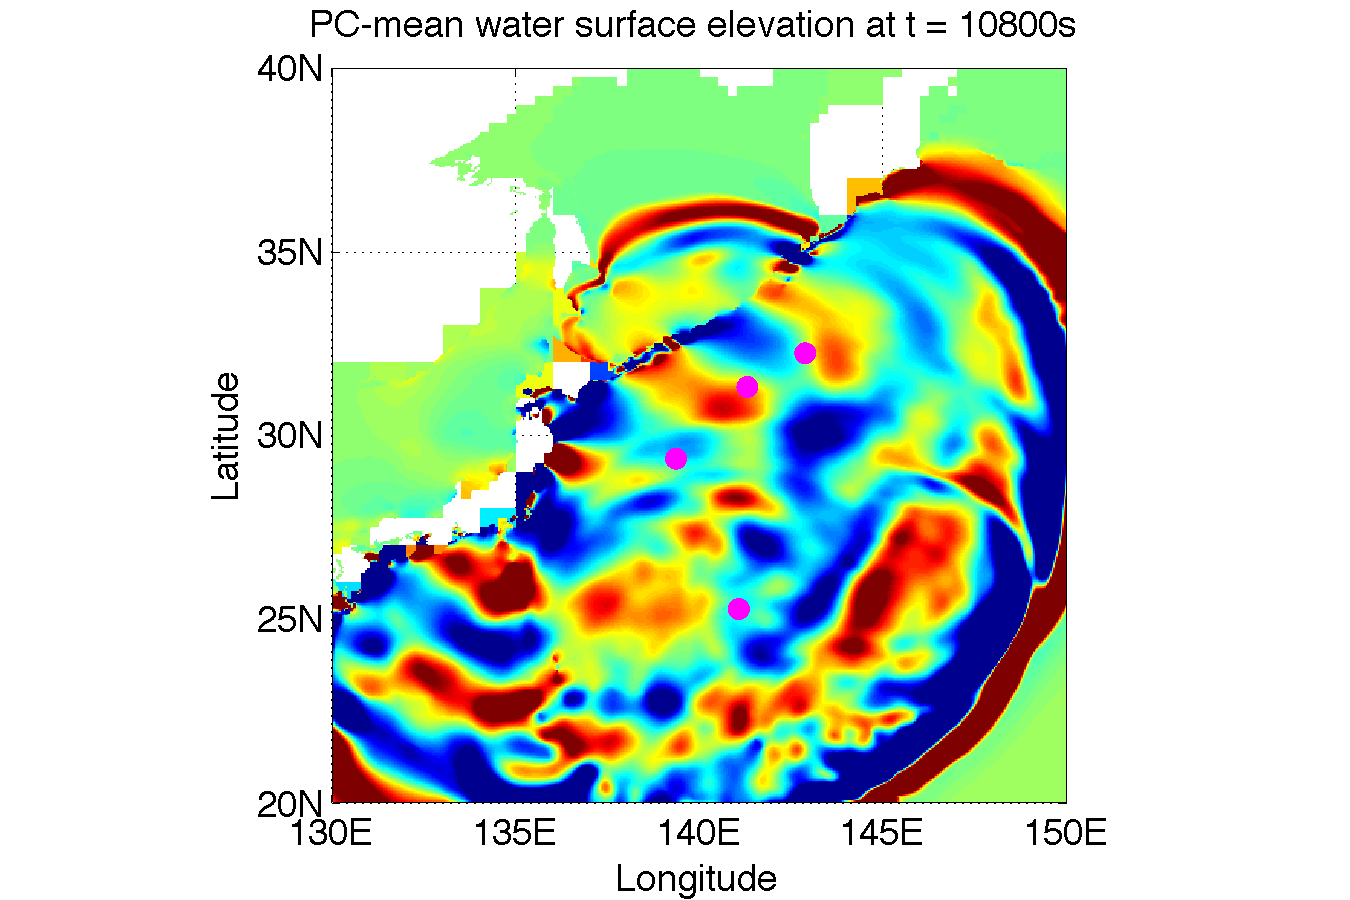
\includegraphics[width=0.45\textwidth]{Figure9b.pdf} &
\hspace*{-45pt}
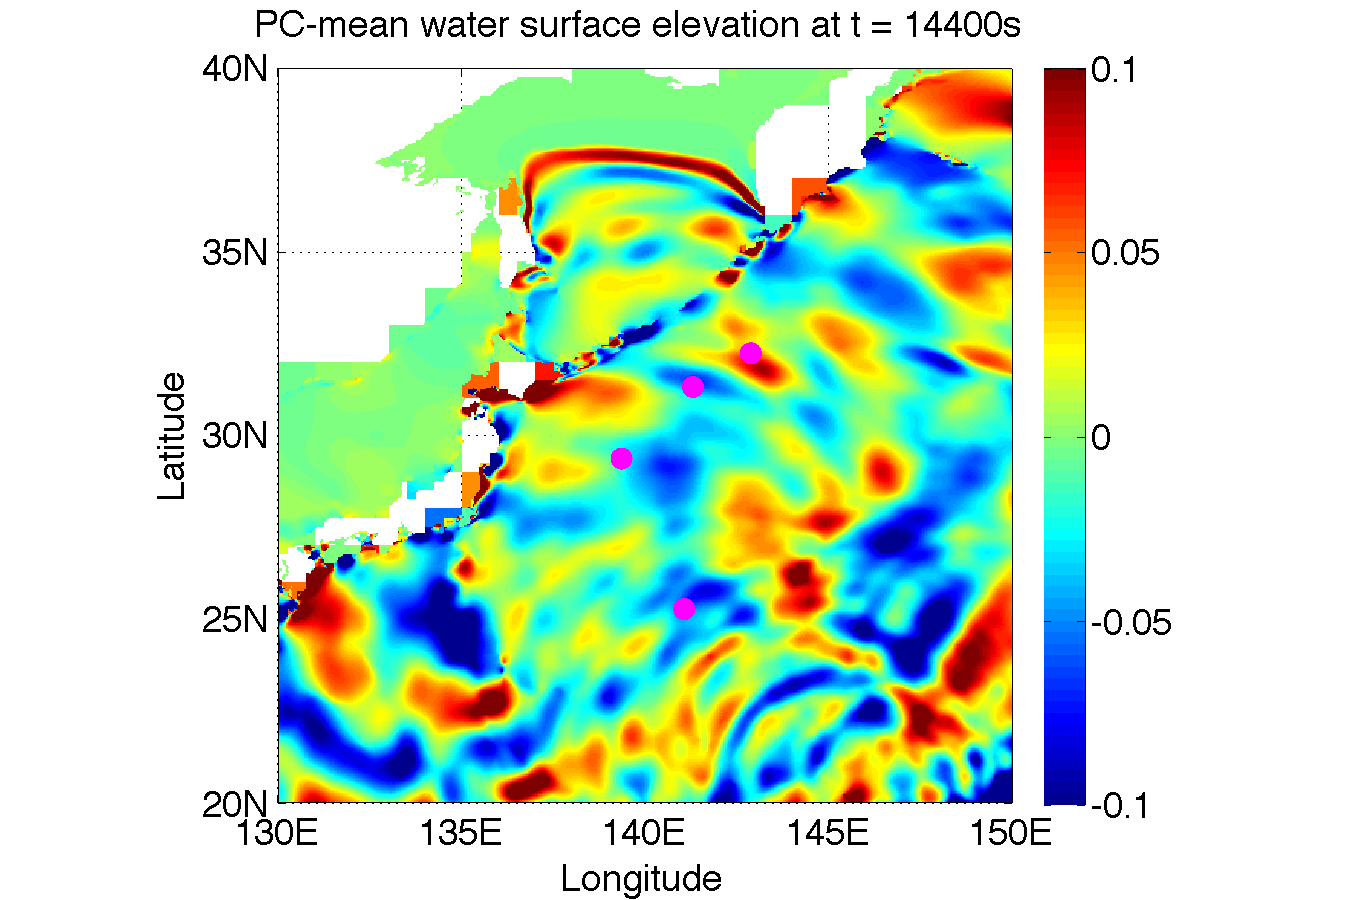
\includegraphics[width=0.45\textwidth]{Figure9c.pdf} \\
\hspace*{-55pt}
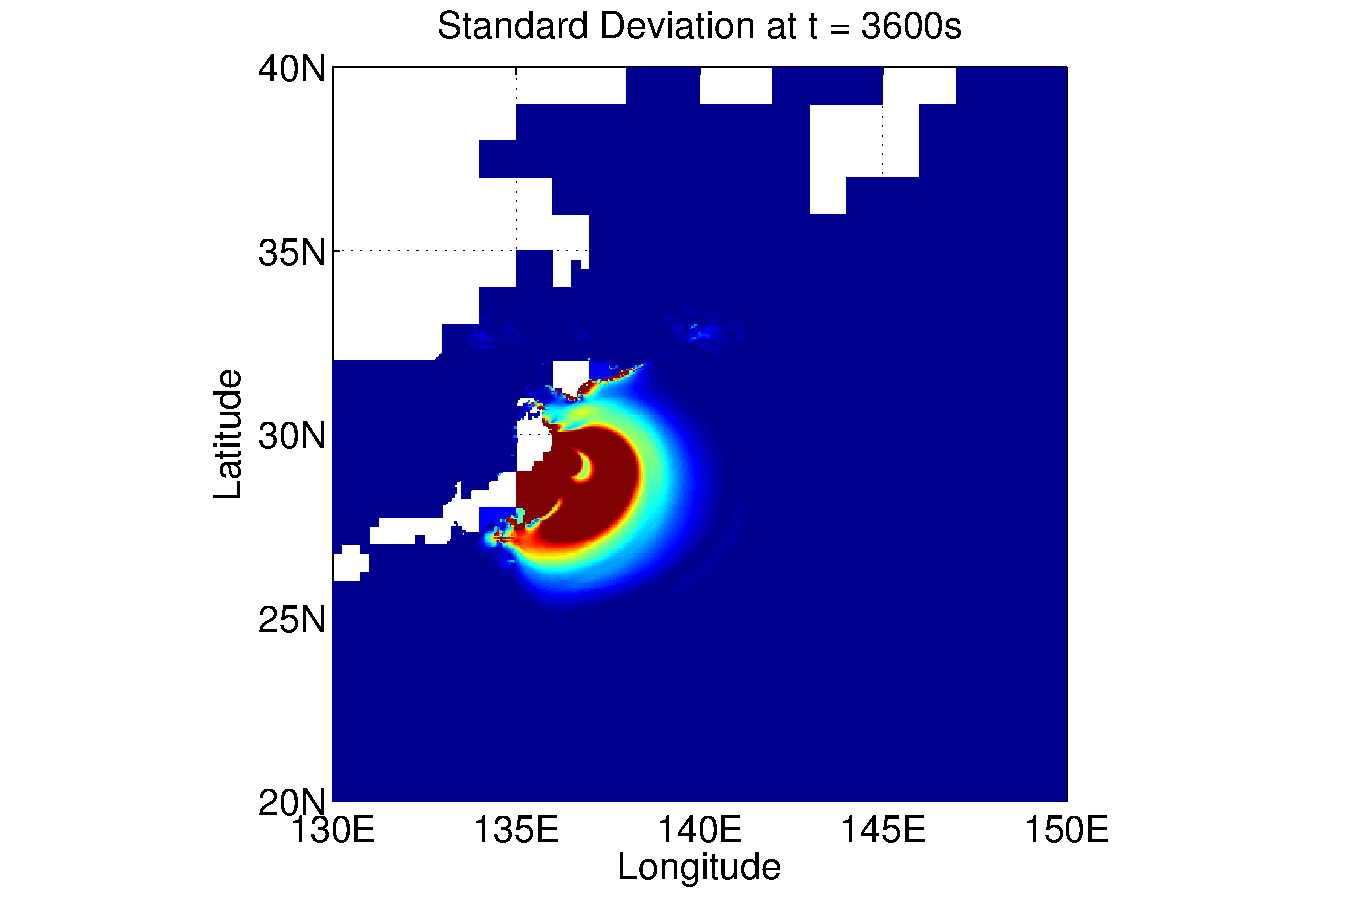
\includegraphics[width=0.45\textwidth]{Figure9d.pdf} &
\hspace*{-45pt}
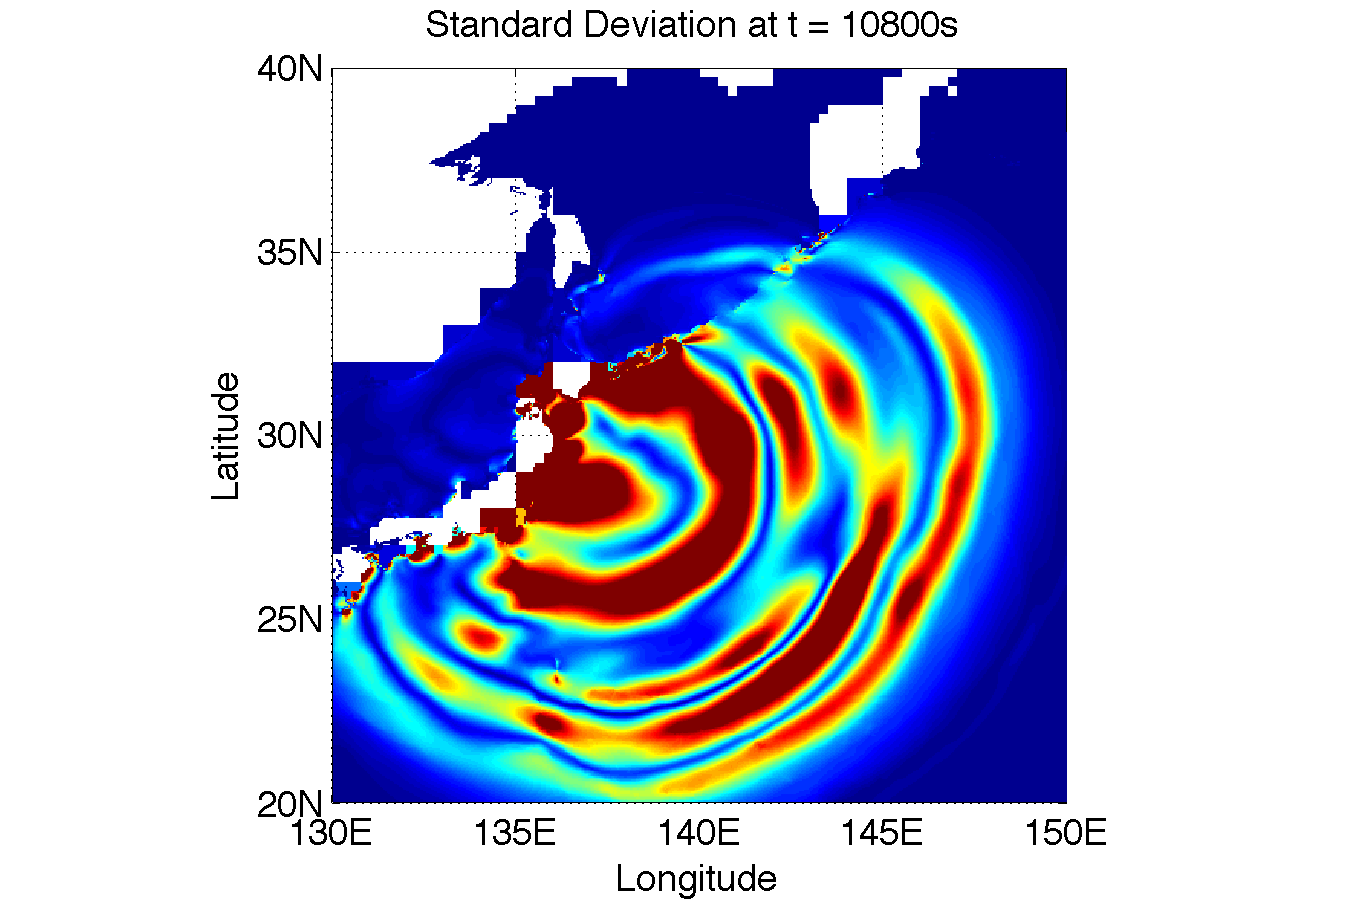
\includegraphics[width=0.45\textwidth]{Figure9e.pdf} &
\hspace*{-45pt}
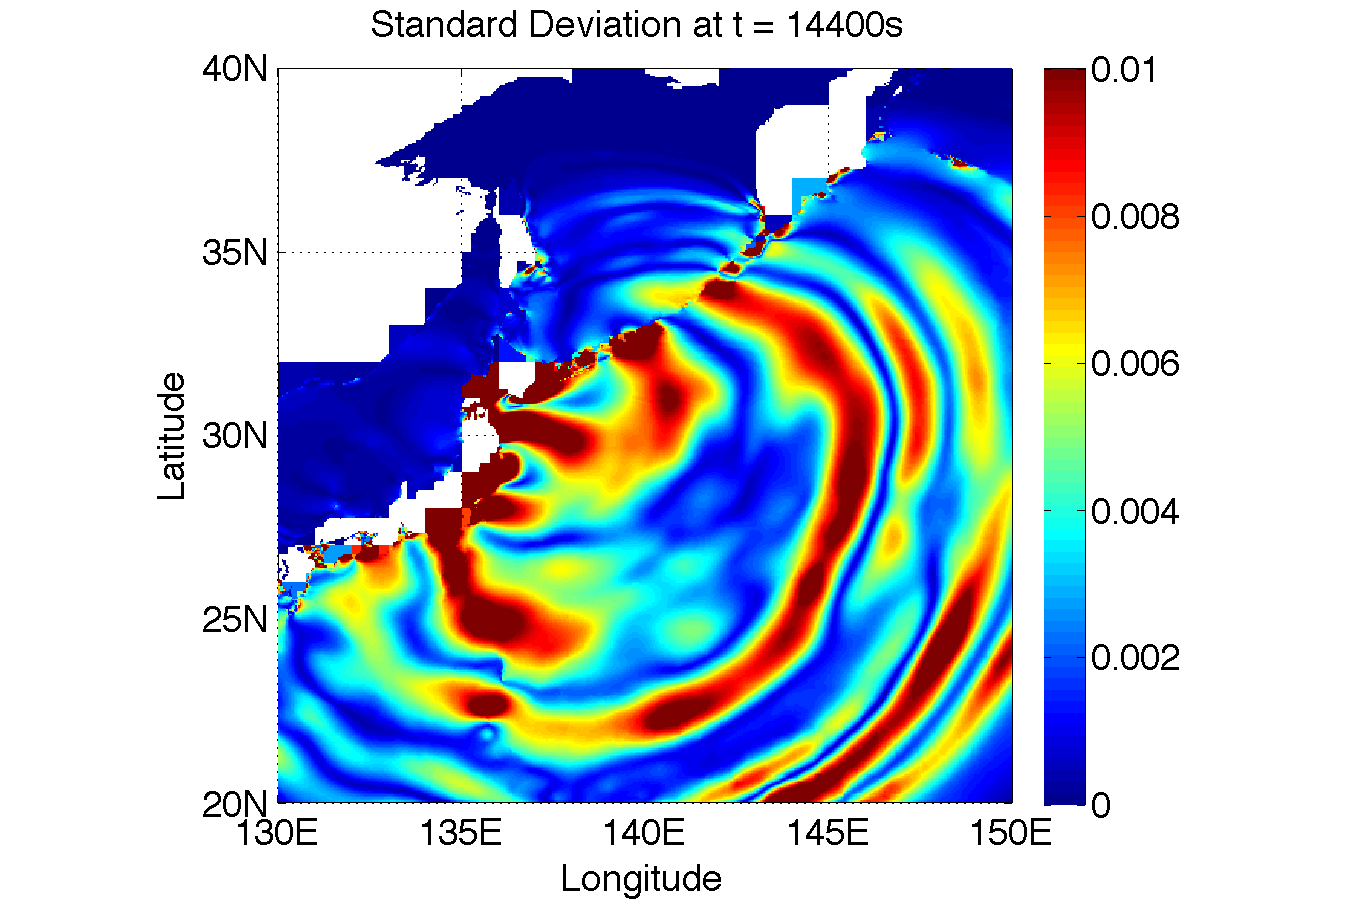
\includegraphics[width=0.45\textwidth]{Figure9f.pdf}
\end{tabular}
\caption{PC mean (top row) and standard deviation (bottom row) of the water surface elevation at different times.}
\label{fig:mean2d}
\end{figure}
%%%%%%%%%%%%%%%%%%%%%%%%%%%%%%%%%%%%%%%%%%%%%%%%%%%%%%%%%%%%%%%%

\begin{figure}[ht]
\begin{tabular}{clc}
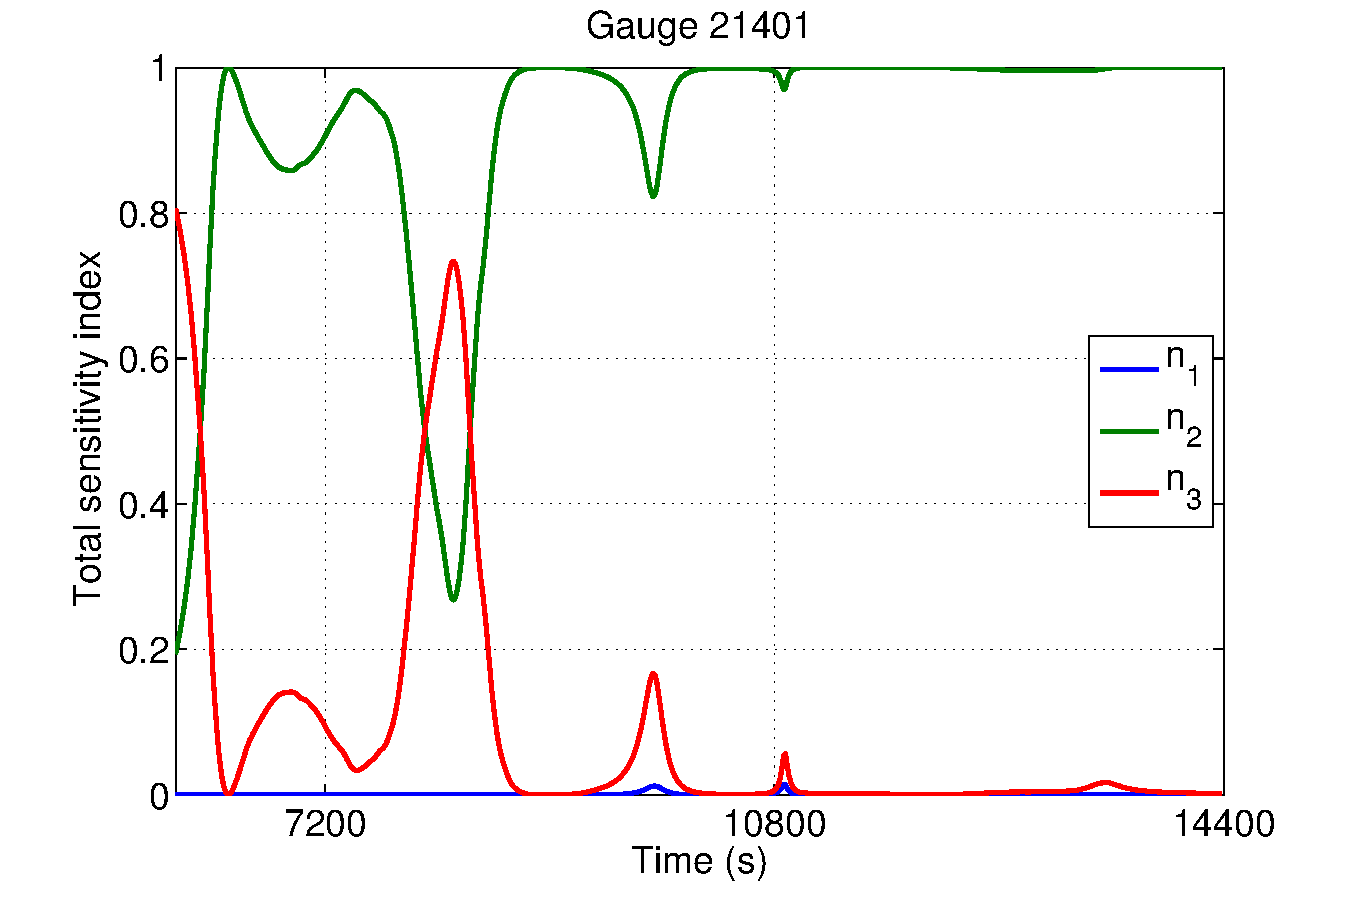
\includegraphics[width=0.475\textwidth]{Figure10a.pdf} &
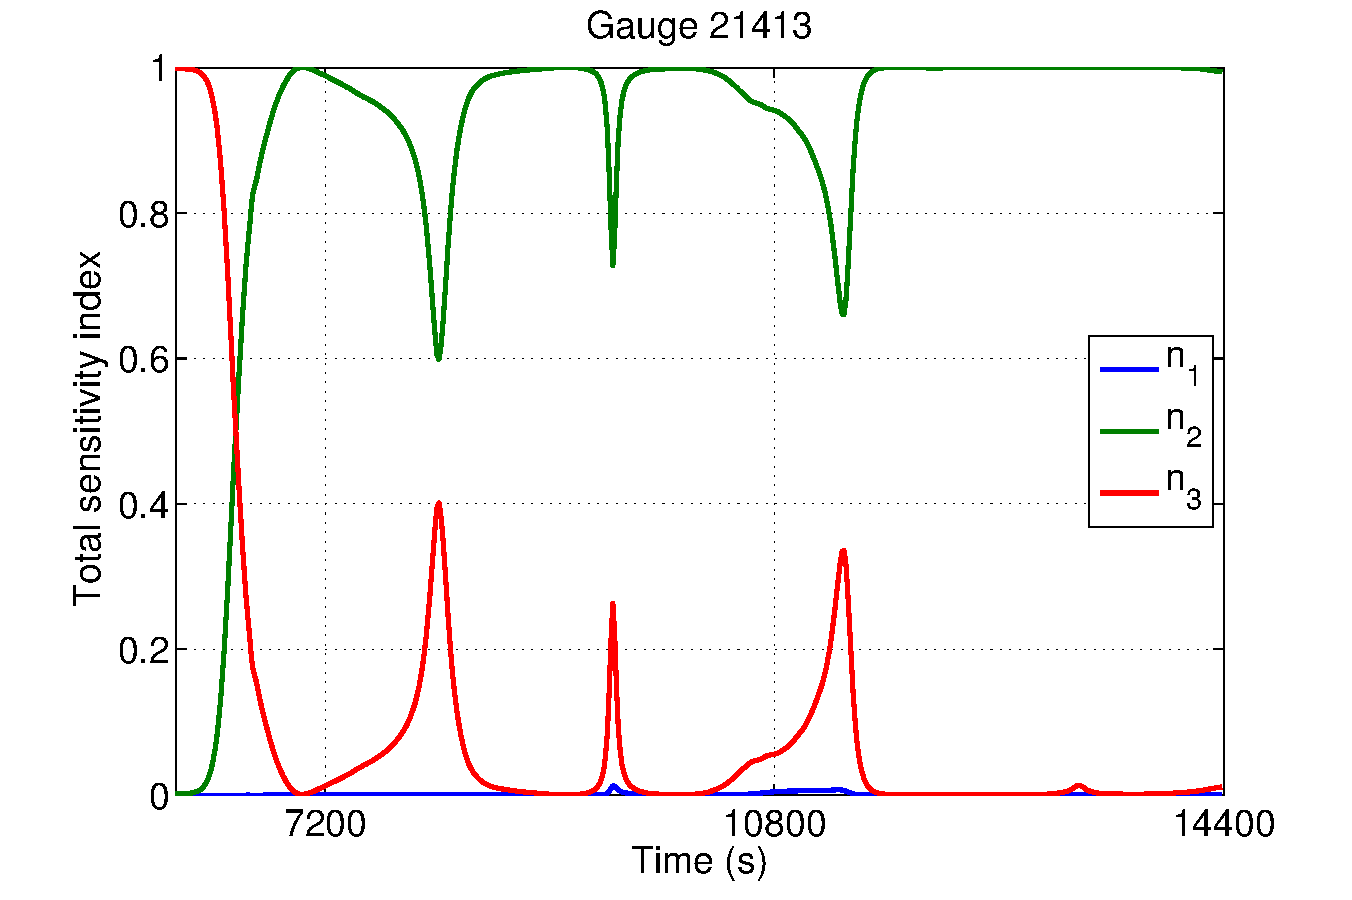
\includegraphics[width=0.475\textwidth]{Figure10b.pdf} \\
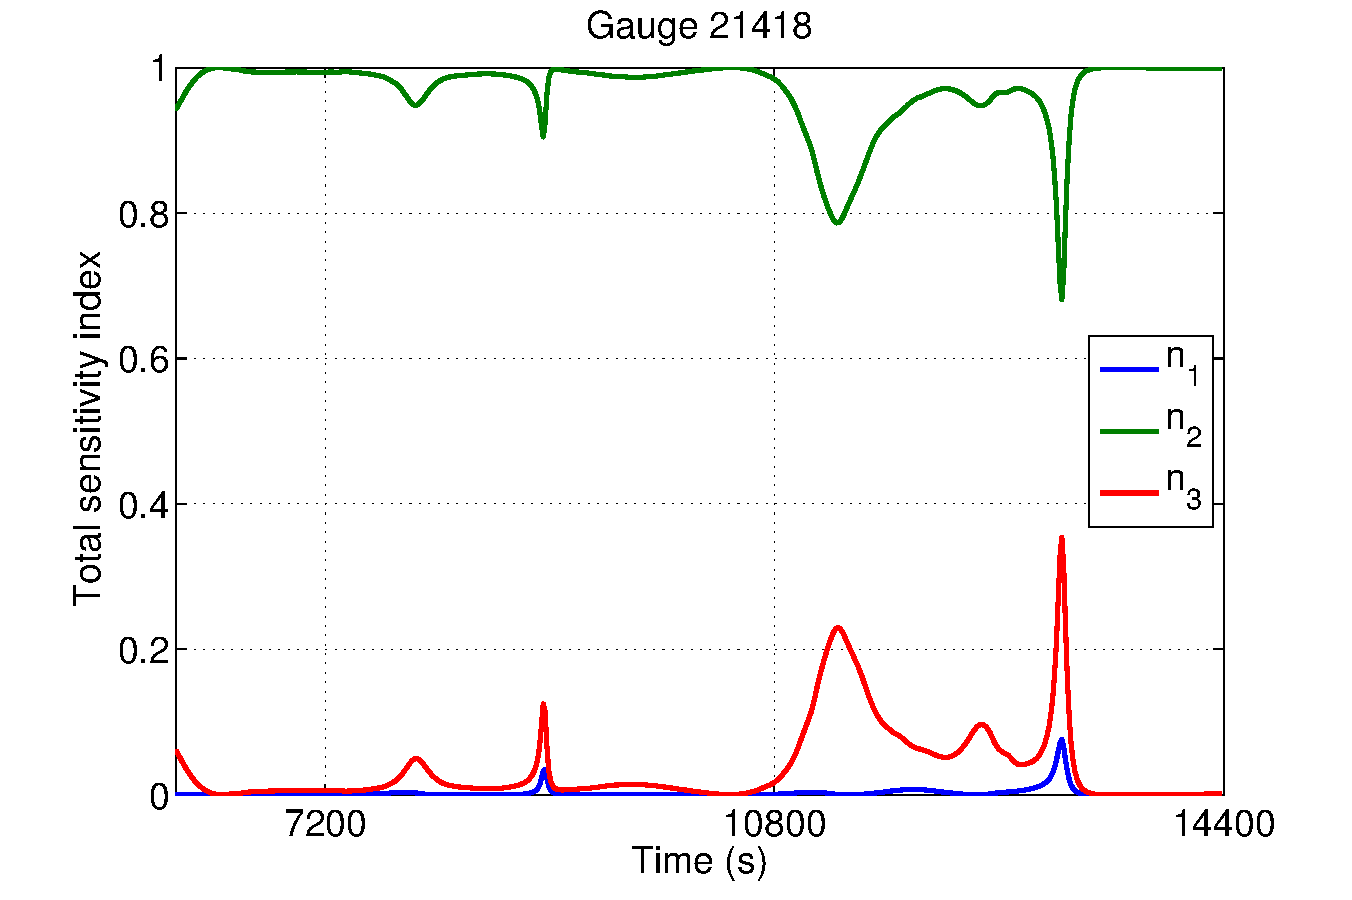
\includegraphics[width=0.475\textwidth]{Figure10c.pdf} &
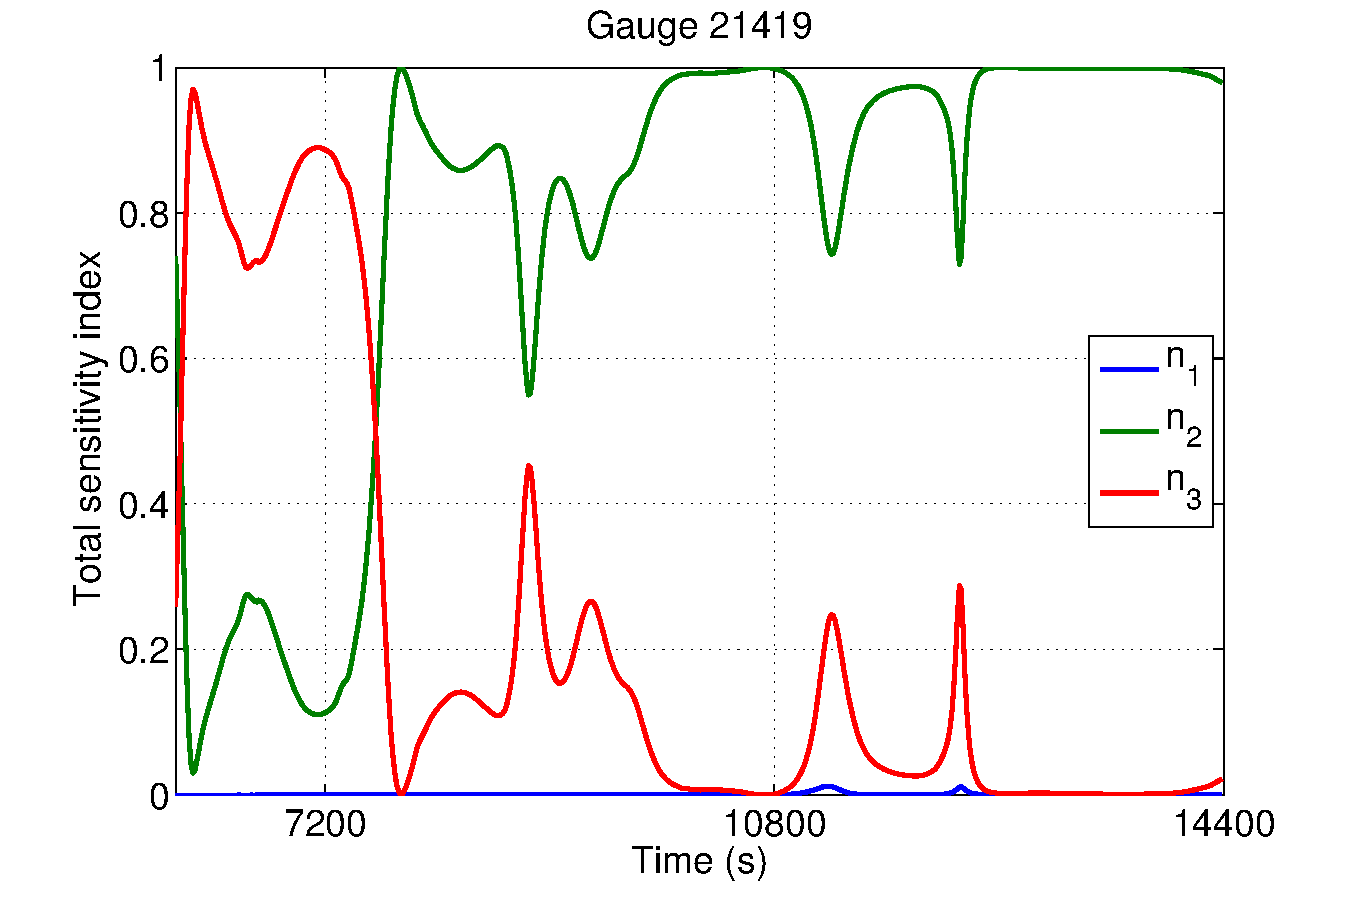
\includegraphics[width=0.475\textwidth]{Figure10d.pdf}
\end{tabular}
\caption{Total sensitivity index of different input parameters.}
\label{fig:sens}
\end{figure}
%%%%%%%%%%%%%%%%%%%%%%%%%%%%%%%%%%%%%%%%%%%%%%%%%%%%%%%%%%%%%%%%

\begin{figure}[ht]
\begin{tabular}{clc}
 \hspace*{-55pt}
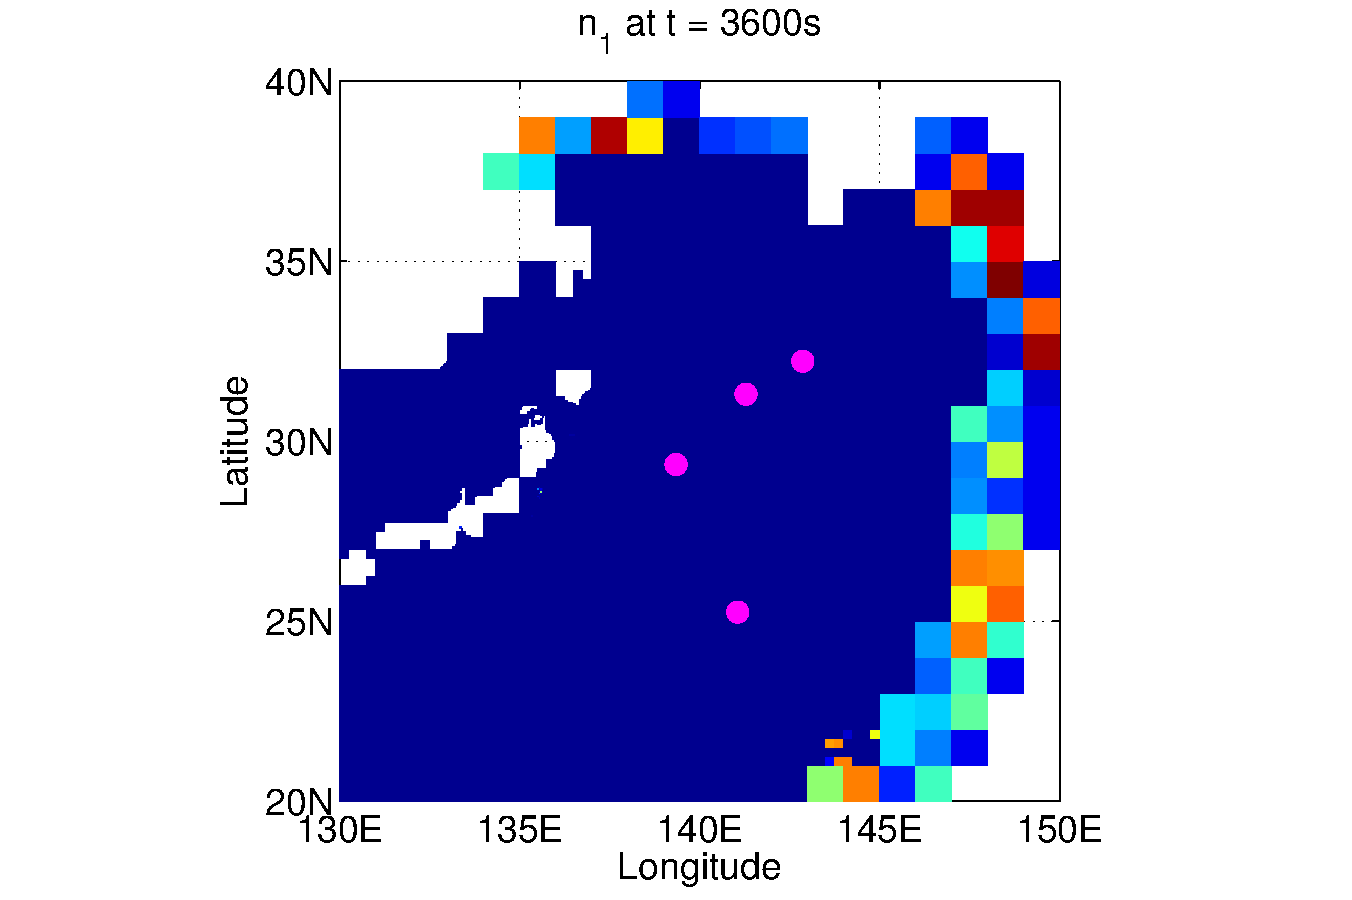
\includegraphics[width=0.45\textwidth]{Figure11a.pdf} &
\hspace*{-45pt}
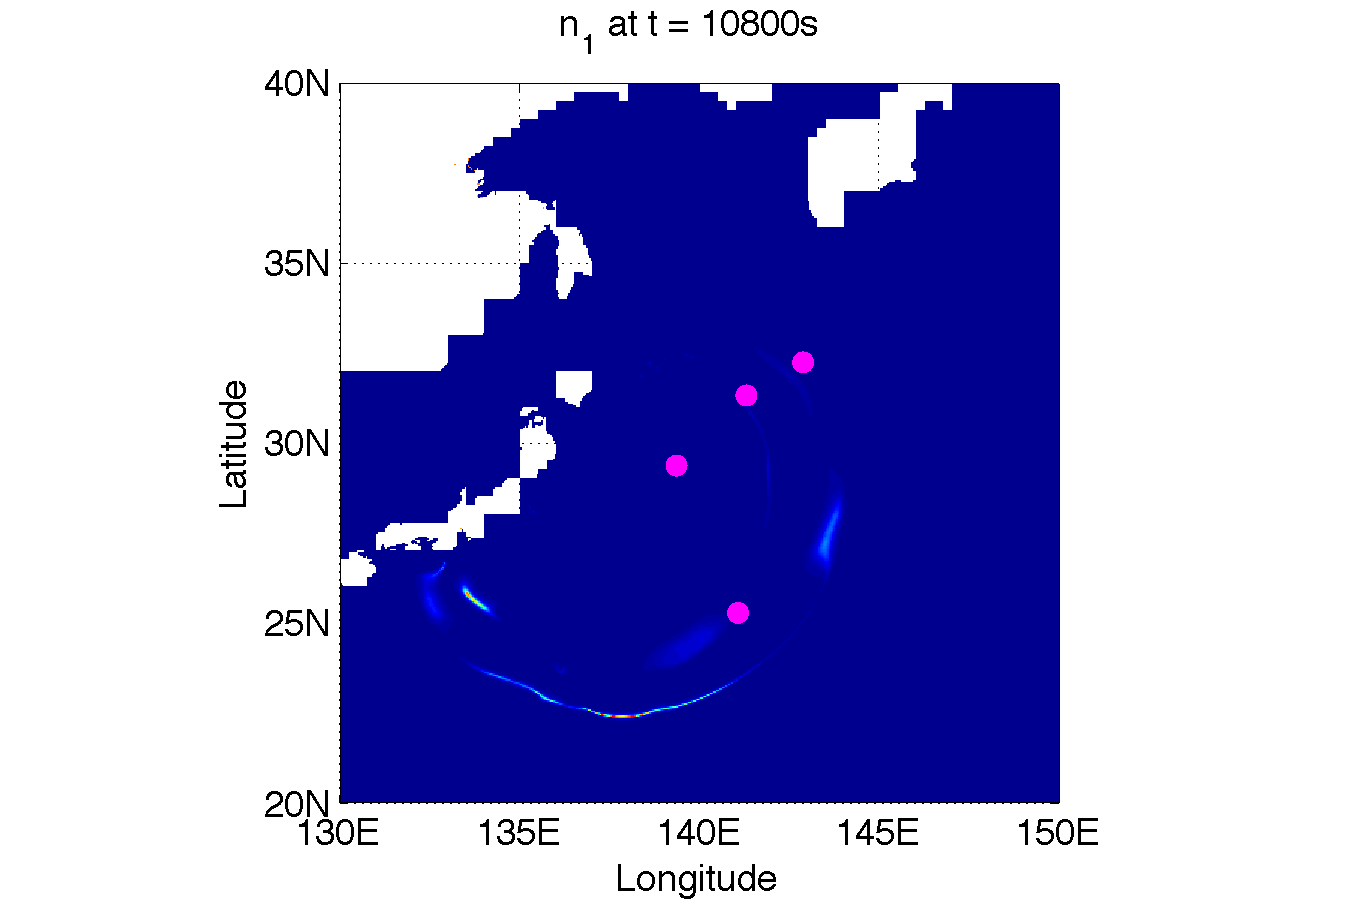
\includegraphics[width=0.45\textwidth]{Figure11b.pdf} &
\hspace*{-45pt}
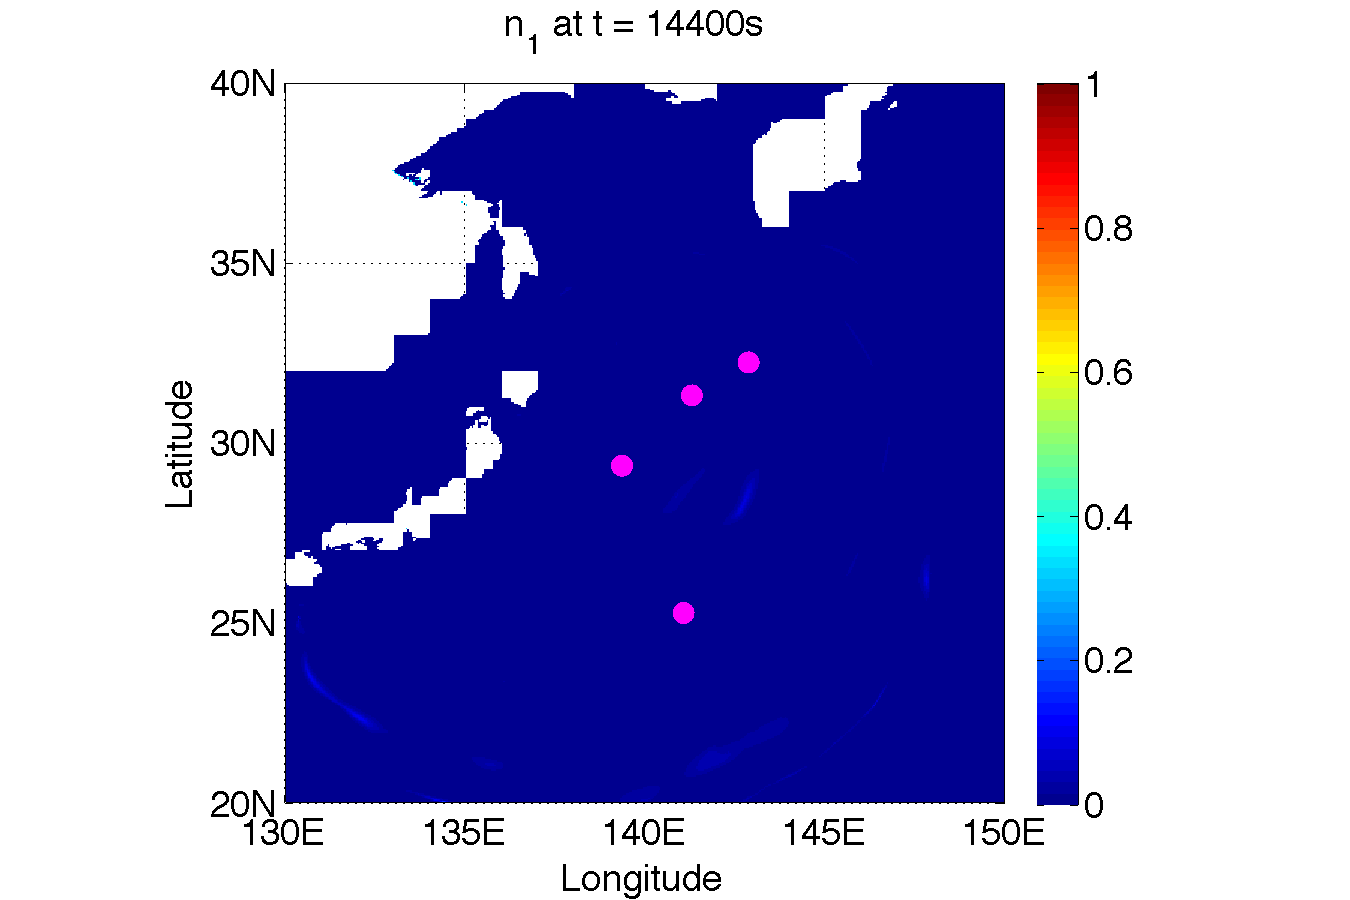
\includegraphics[width=0.45\textwidth]{Figure11c.pdf} \\
\hspace*{-55pt}
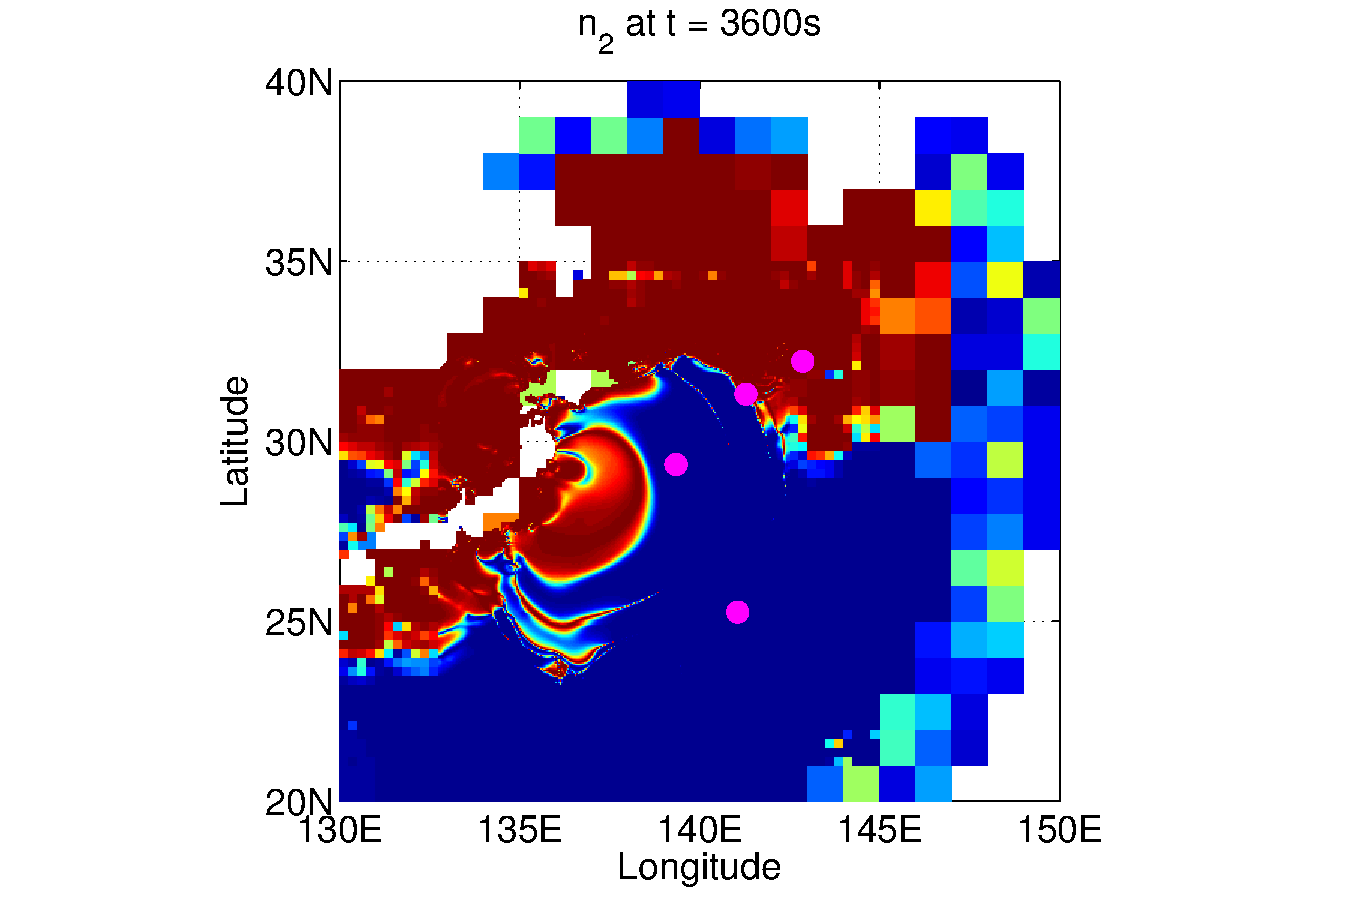
\includegraphics[width=0.45\textwidth]{Figure11d.pdf} &
\hspace*{-45pt}
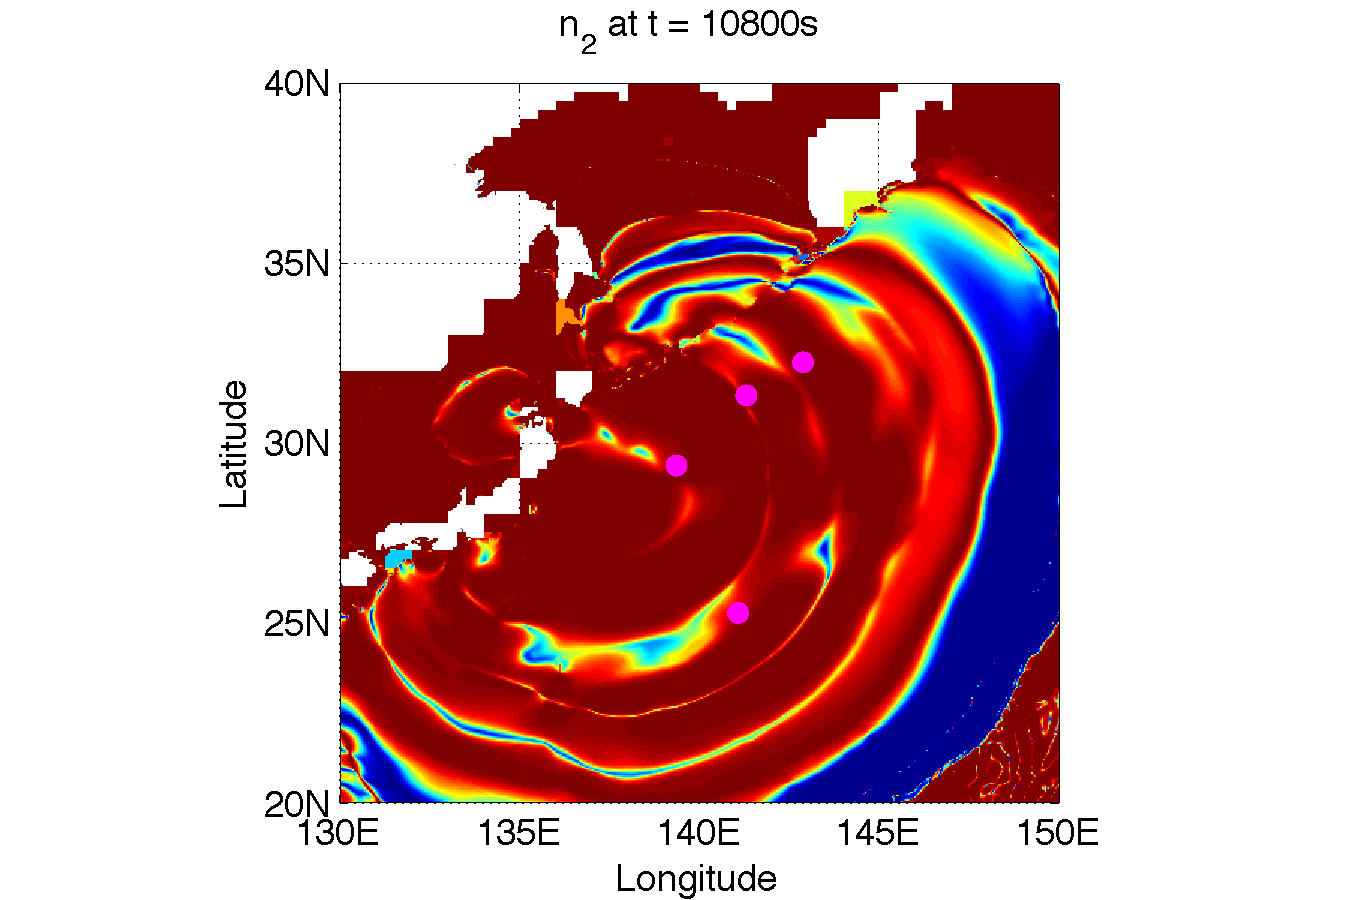
\includegraphics[width=0.45\textwidth]{Figure11e.pdf} &
\hspace*{-45pt}
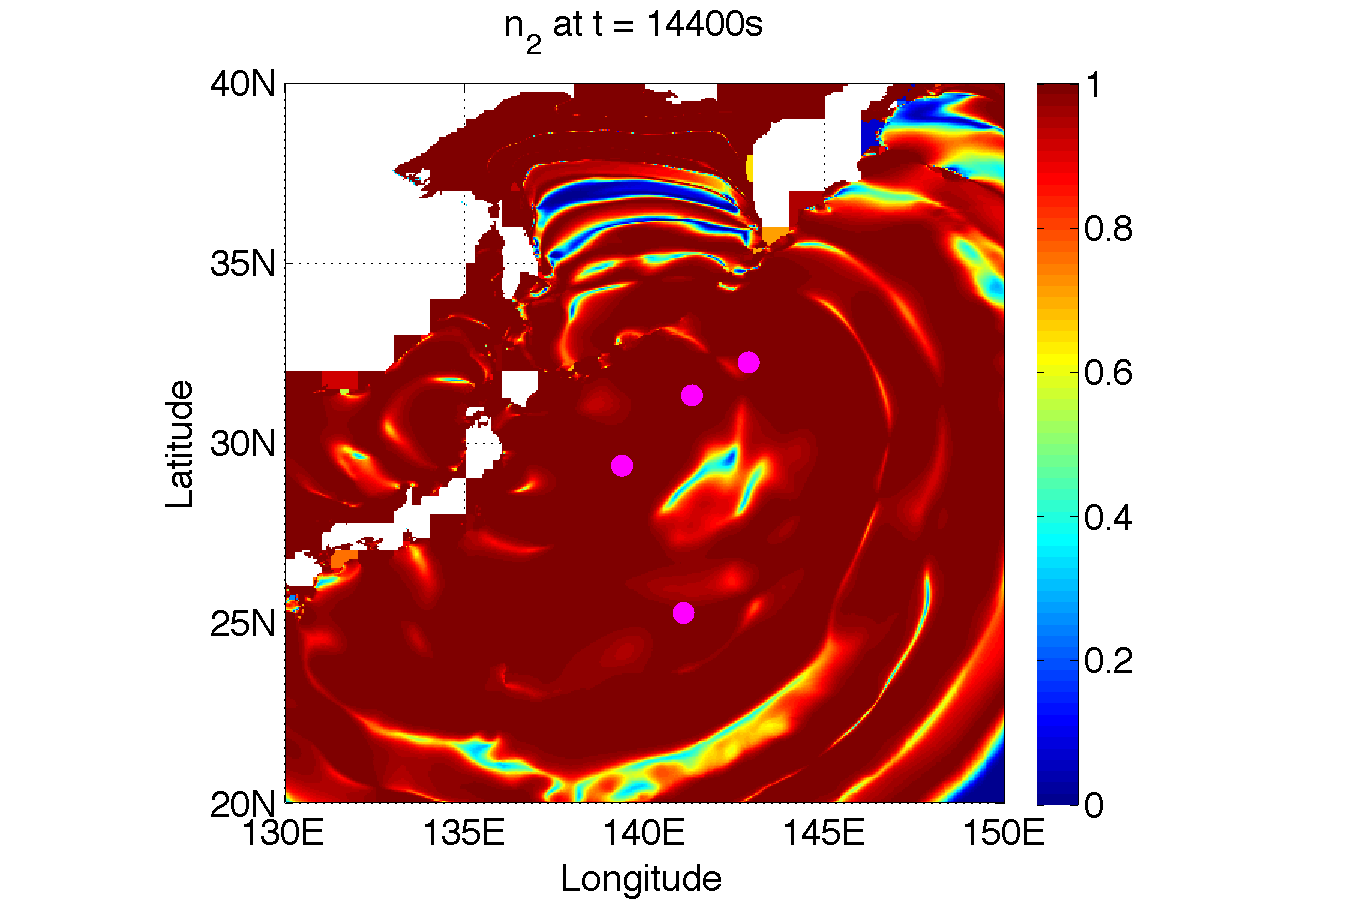
\includegraphics[width=0.45\textwidth]{Figure11f.pdf} \\
\hspace*{-55pt}
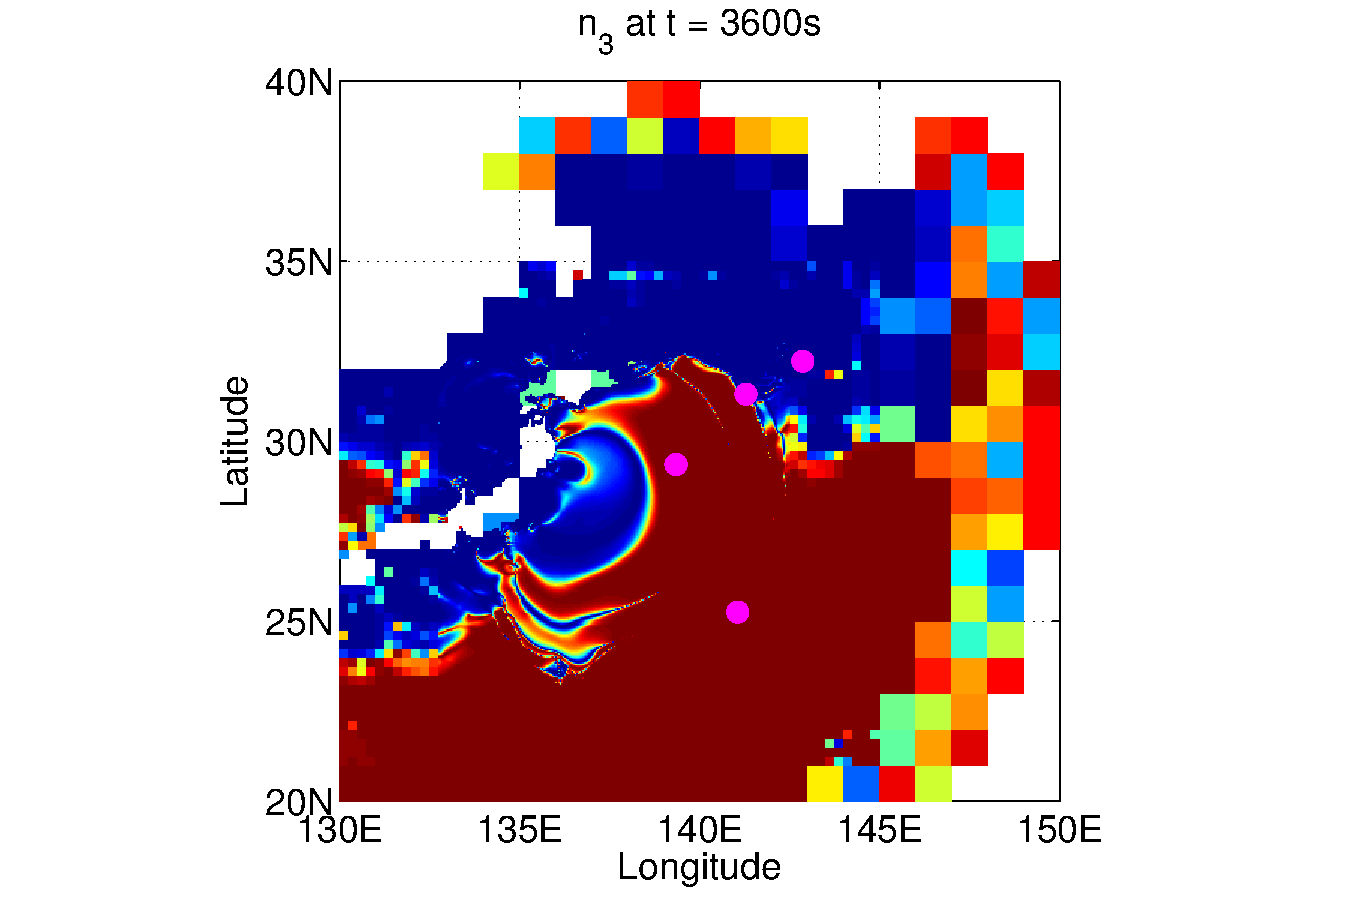
\includegraphics[width=0.45\textwidth]{Figure11g.pdf} &
\hspace*{-45pt}
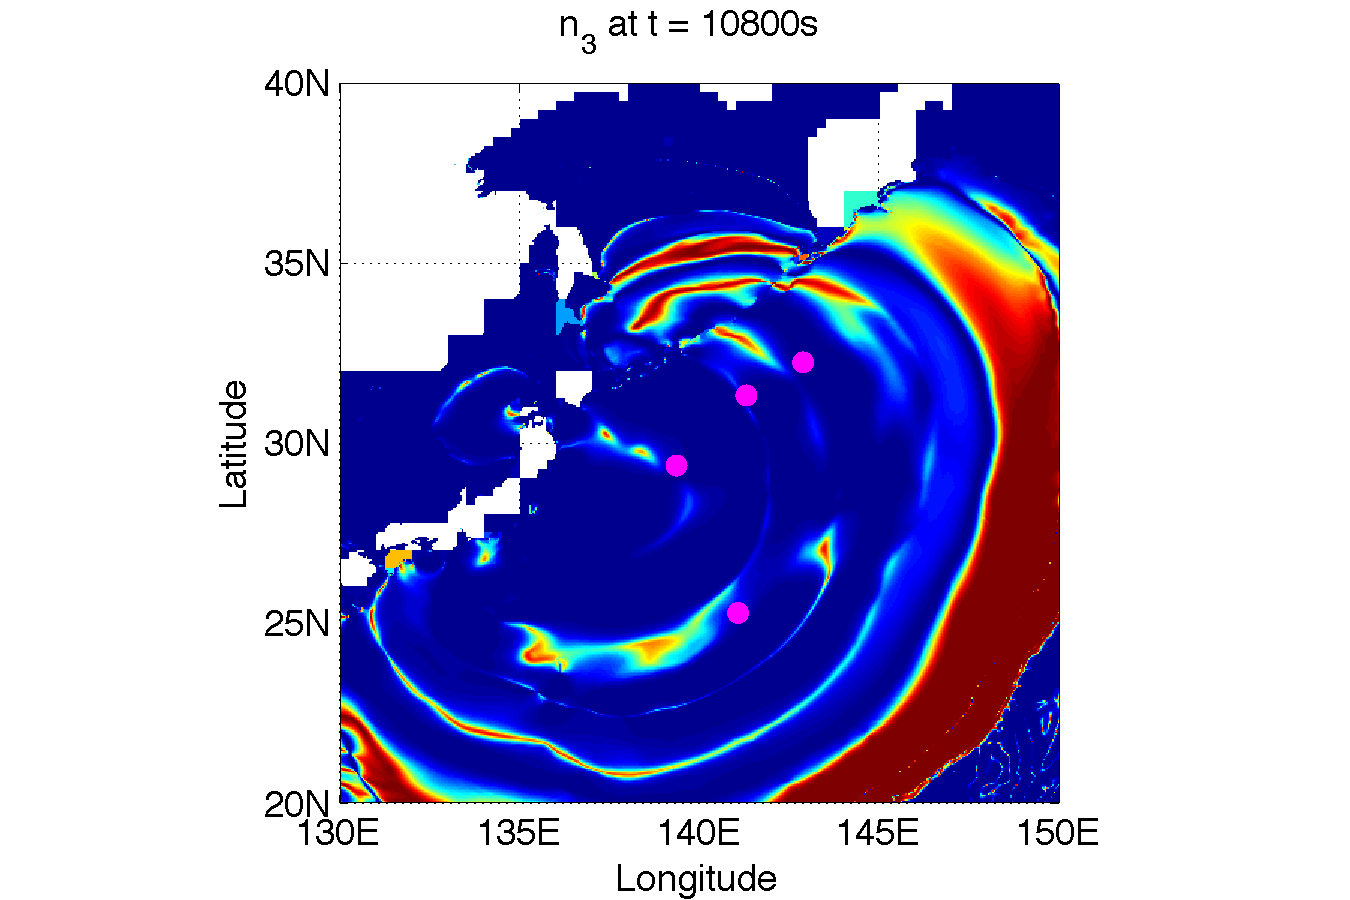
\includegraphics[width=0.45\textwidth]{Figure11h.pdf} &
\hspace*{-45pt}
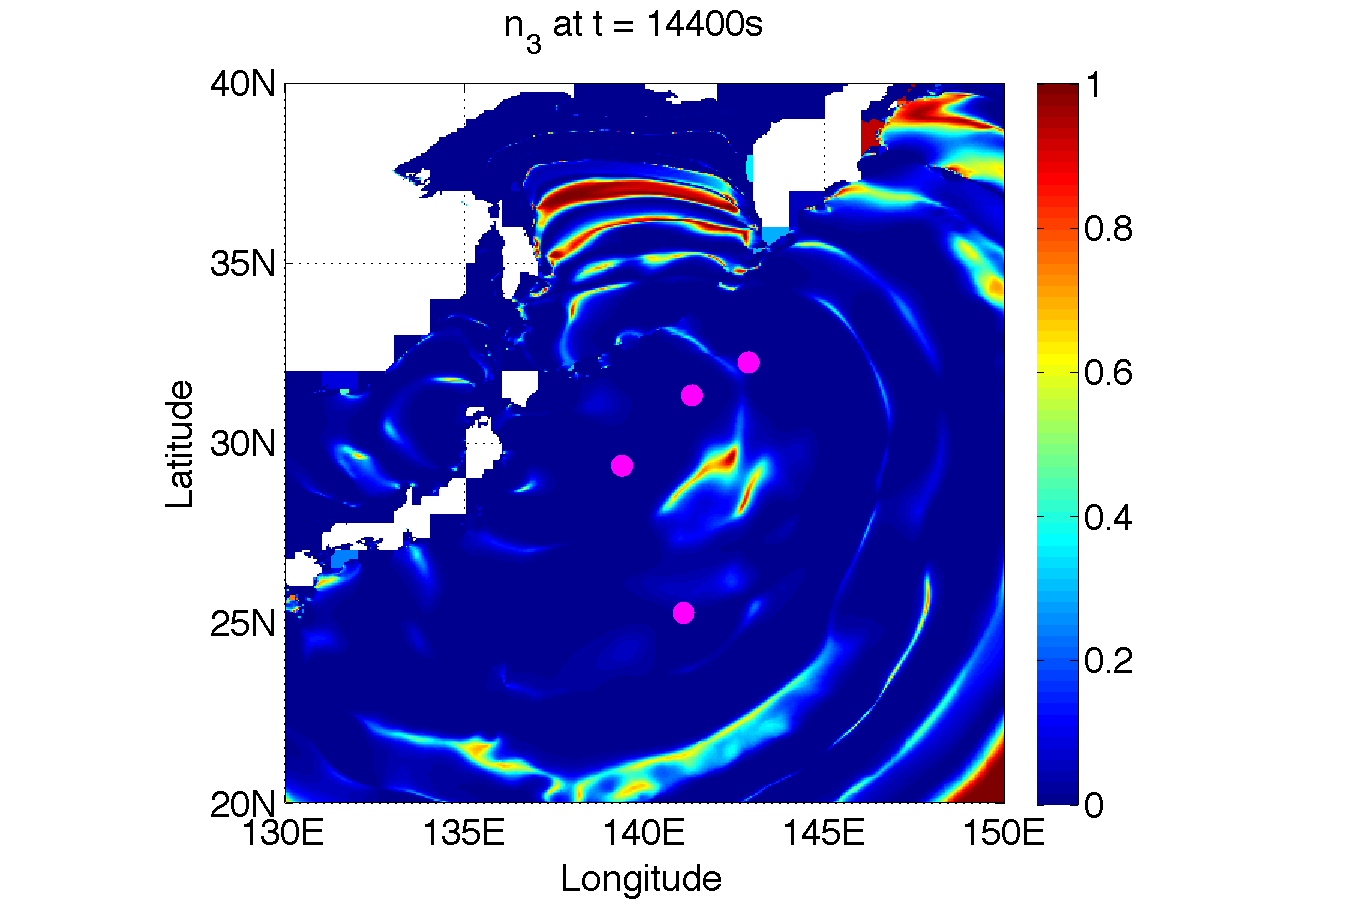
\includegraphics[width=0.45\textwidth]{Figure11i.pdf}
\end{tabular}
\caption{Total sensitivity index for $n_1$ (top row) $n_2$ (center row) and $n_3$ (bottom row)
 at different times as indicated.}
\label{fig:sens2d}
\end{figure}
%%%%%%%%%%%%%%%%%%%%%%%%%%%%%%%%%%%%%%%%%%%%%%%%%%%%%%%%%%%%%%%%
\begin{figure}[ht]
\centering

\begin{tabular}{clcl}
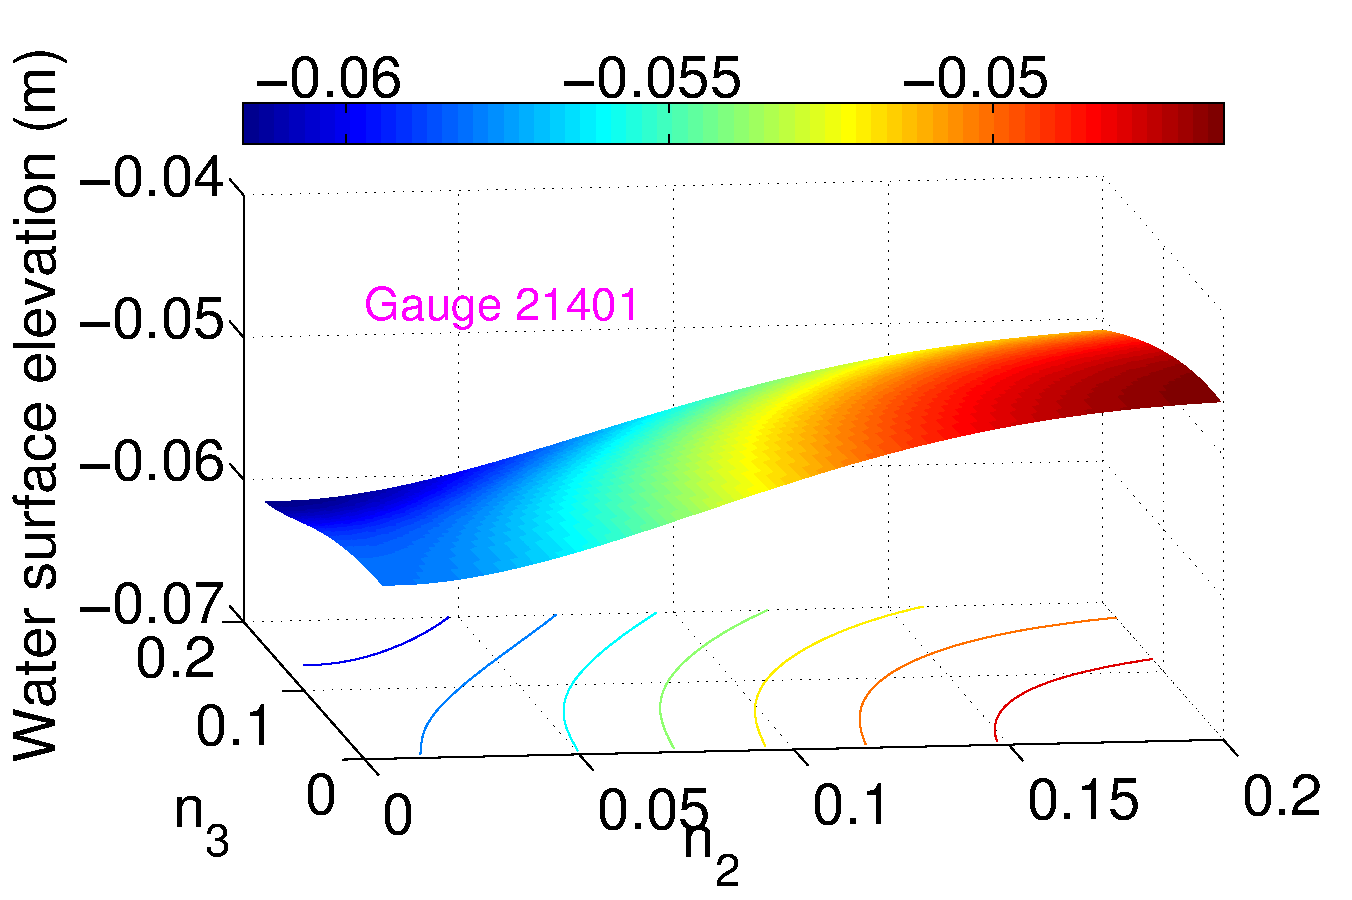
\includegraphics[width=0.5\textwidth]{Figure12a.pdf} &
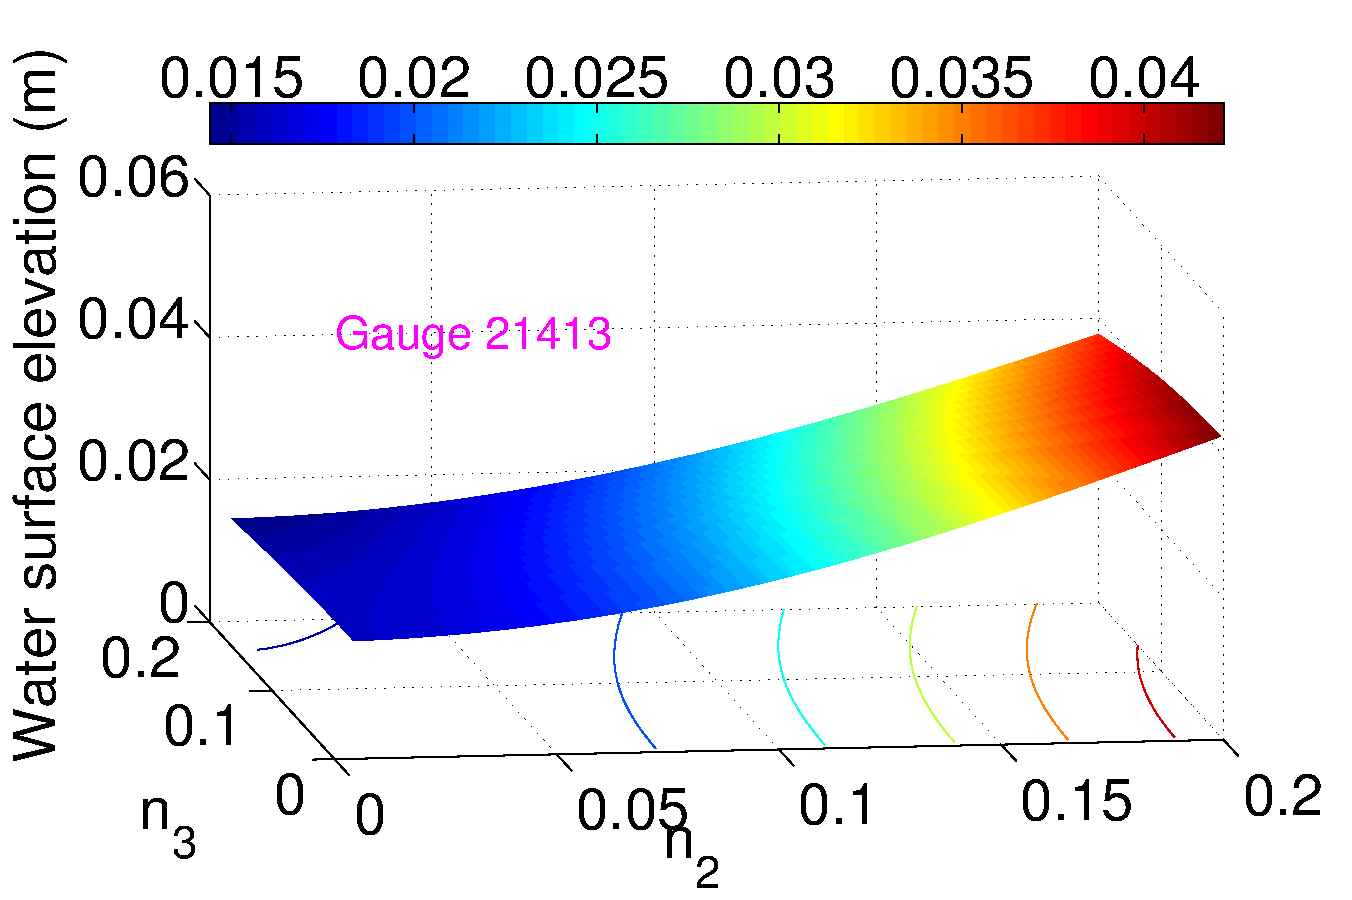
\includegraphics[width=0.5\textwidth]{Figure12b.pdf} \\
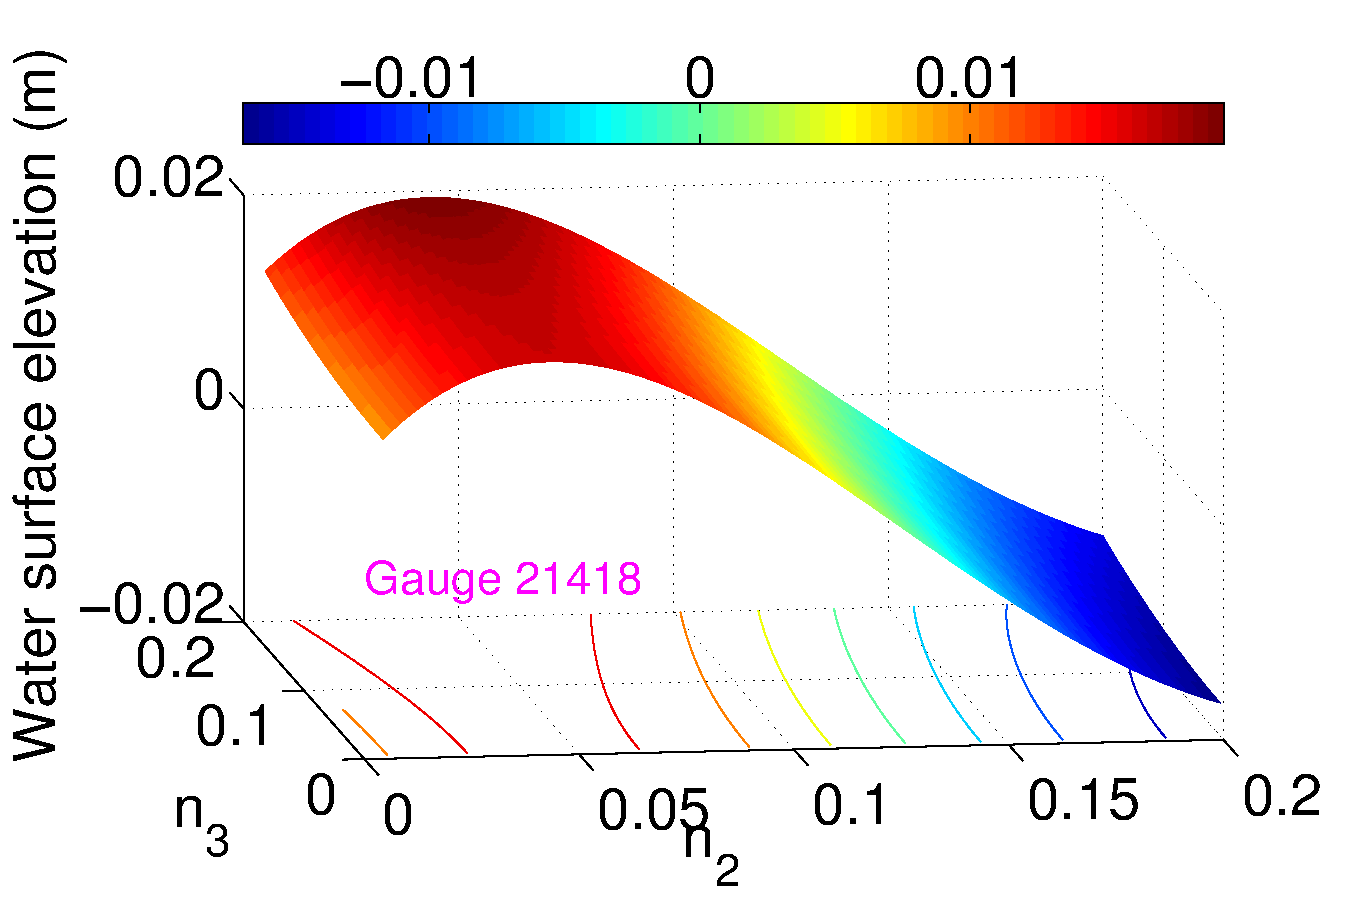
\includegraphics[width=0.5\textwidth]{Figure12c.pdf} &
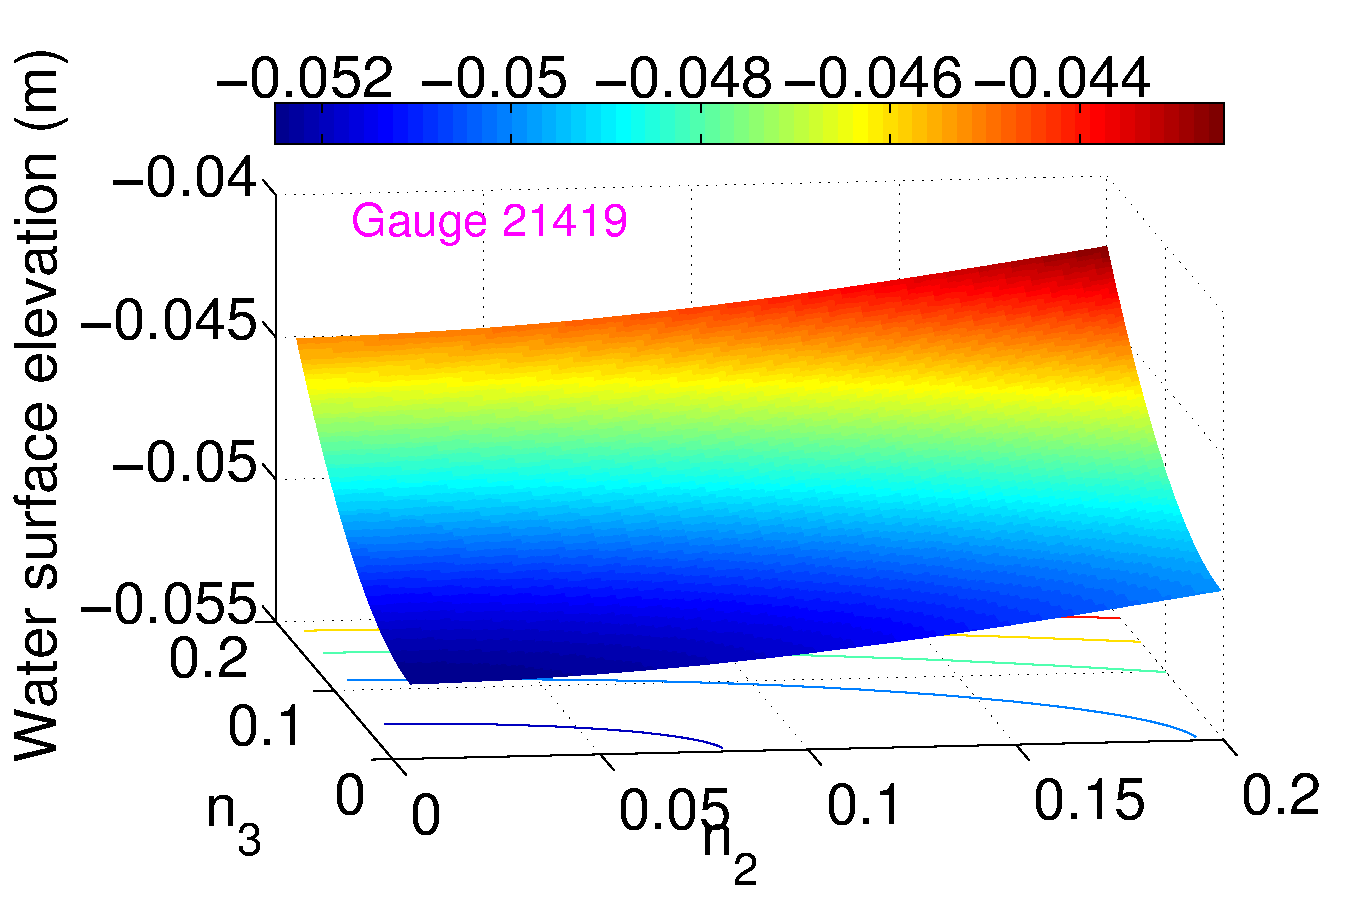
\includegraphics[width=0.5\textwidth]{Figure12d.pdf}
\end{tabular}
\caption{Response surface of water surface elevation at the different gauge locations at t = 7200 s
as function of $n_2$ and $n_3$, with fixed $n_1=0.035$}.
\label{fig:response2}
\end{figure}
%%%%%%%%%%%%%%%%%%%%%%%%%%%%%%%%%%%%%%%%%%%%%%%%%%%%%%%%%%%%%%%%

\begin{figure}[ht]
\centering
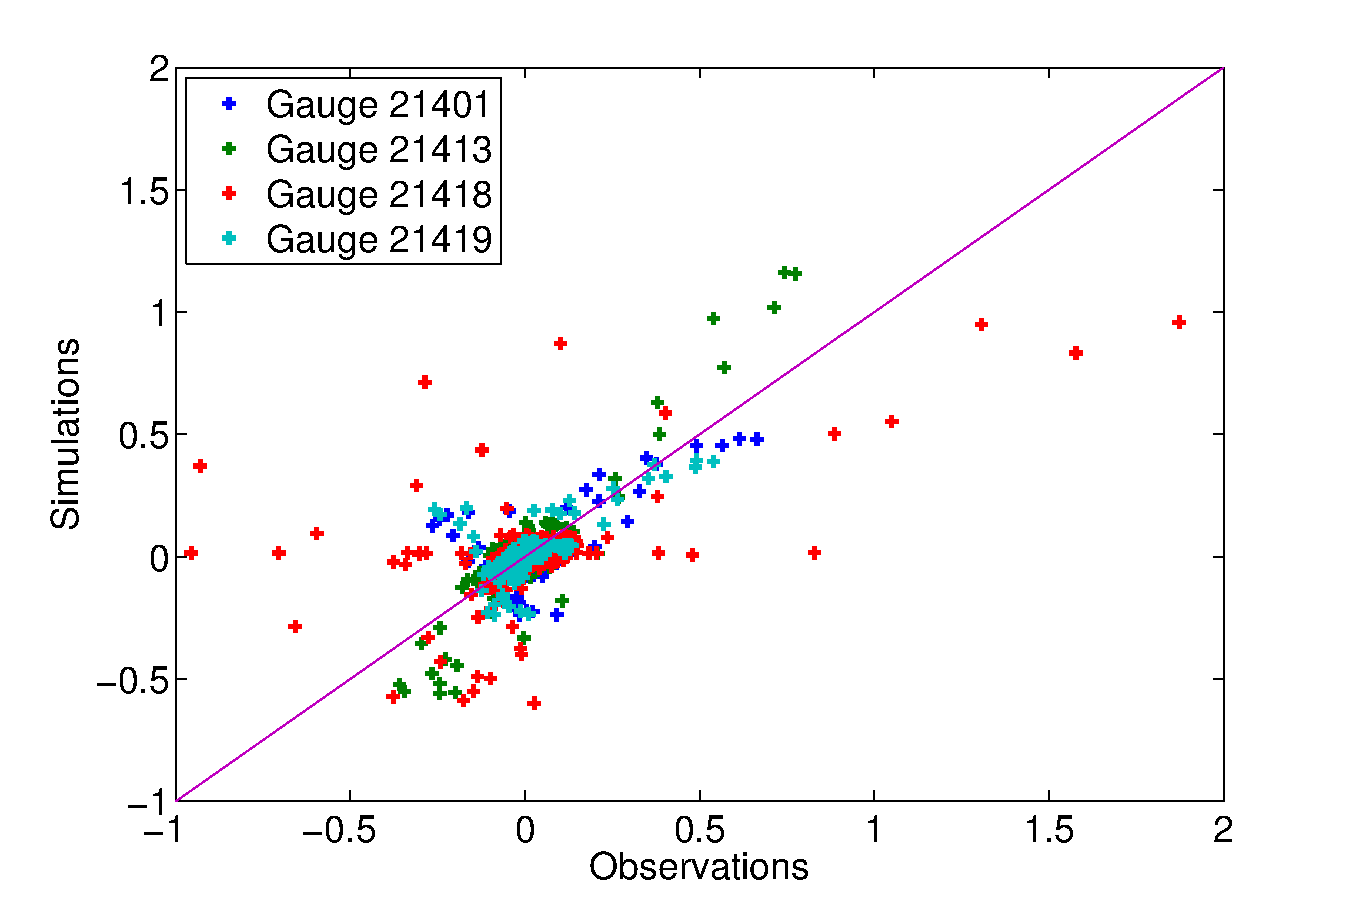
\includegraphics[width=0.575\textwidth]{Figure13.pdf} 
\caption{Scatter plot of measured water surface elevation against their \geoclaw
model counterparts during Tsunami \tohoku. The data points are colored 
differently for the different gauges as indicated in the legend. }
\label{fig:scatter}

\end{figure}  
%%%%%%%%%%%%%%%%%%%%%%%%%%%%%%%%%%%%%%%%%%%%%%%%%%%%%%%%%%%%%%%%
\begin{figure}[ht]
\begin{tabular}{clc}
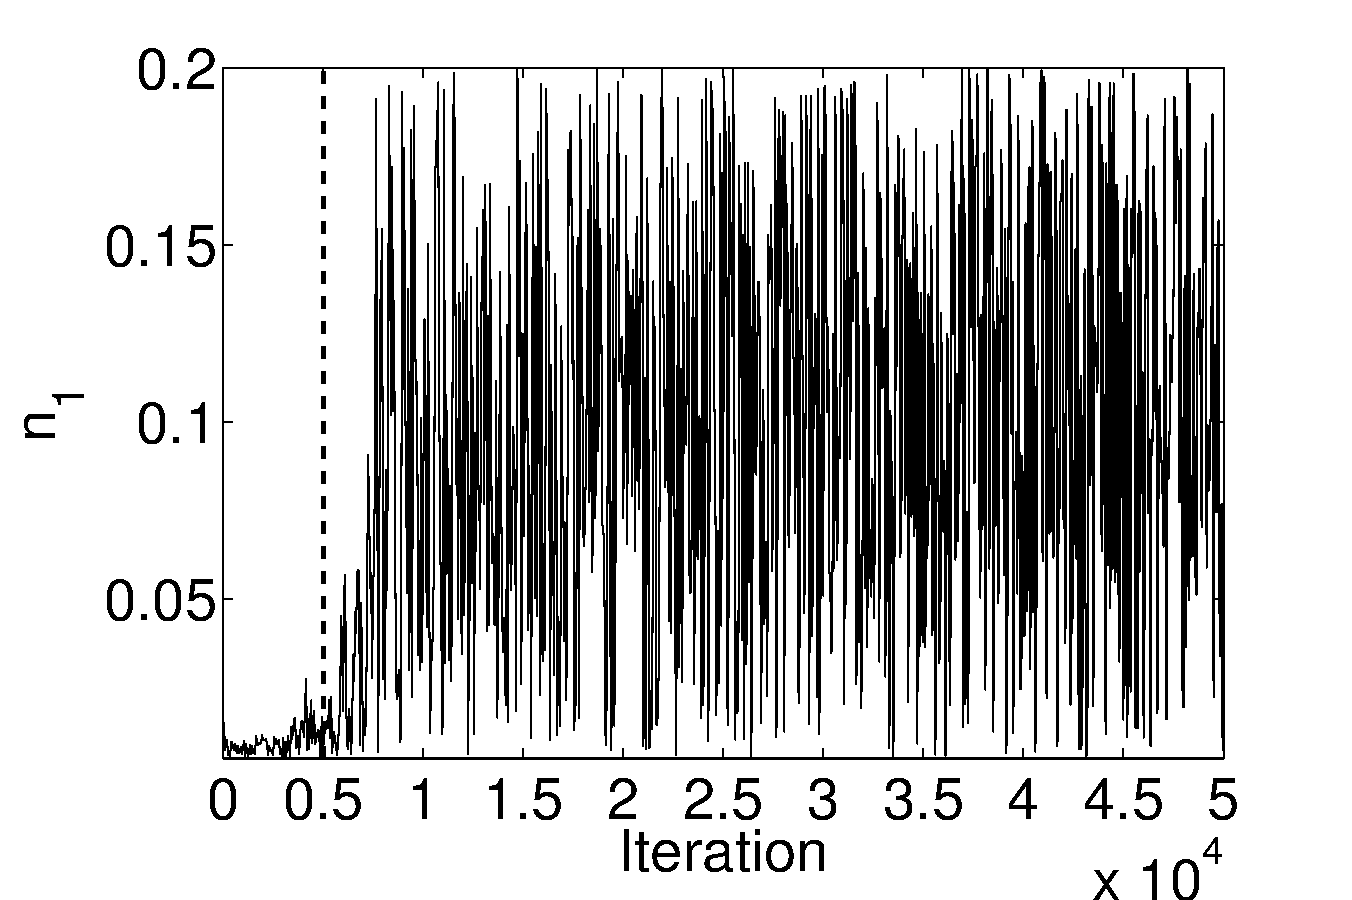
\includegraphics[width=0.475\textwidth]{Figure14a.pdf} &
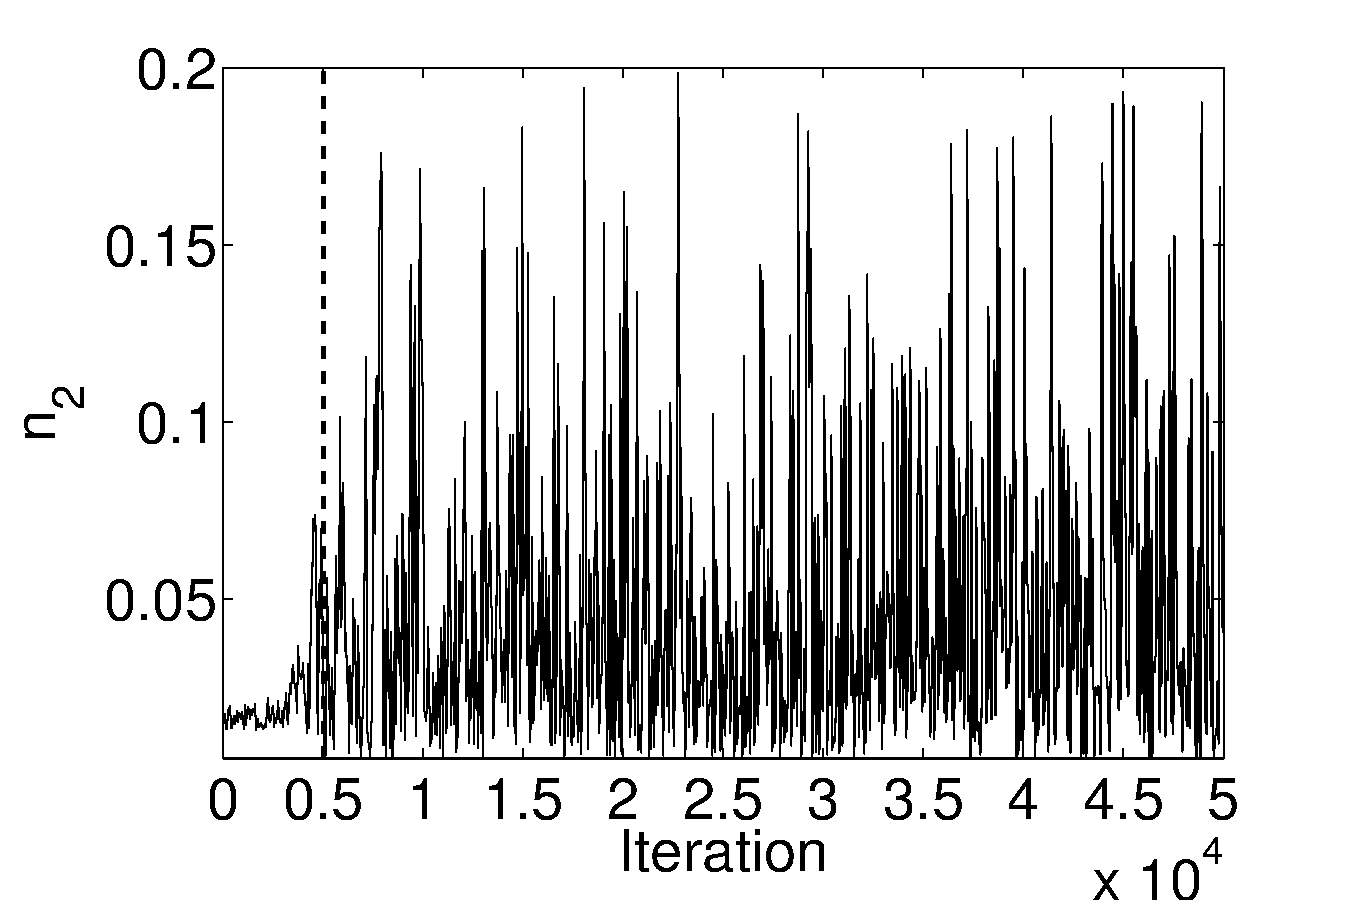
\includegraphics[width=0.475\textwidth]{Figure14b.pdf} \\
\includegraphics[width=0.475\textwidth]{Figure14c.pdf} &
\includegraphics[width=0.475\textwidth]{Figure14d.pdf}
\end{tabular}
\caption{Chain samples for the three Manning's $n$ coefficients $n_1,n_2,n_3$ and $\sigma^2$
the noise variance. The vertical dotted lines corresponds to the
burn-in iterations.}
\label{fig:mcmc} 
\end{figure}
%%%%%%%%%%%%%%%%%%%%%%%%%%%%%%%%%%%%%%%%%%%%%%%%%%%%%%%%%%%%%%%%
 \begin{figure}[ht]
        \begin{tabular}{clc}
\includegraphics[width=0.475\textwidth]{Figure15a.pdf} &
\includegraphics[width=0.475\textwidth]{Figure15b.pdf} \\
\includegraphics[width=0.475\textwidth]{Figure15c.pdf} &
\includegraphics[width=0.475\textwidth]{Figure15d.pdf}
        \end{tabular}
        \caption{KDE of the marginalized posterior distributions for the three Manning's $n$ coefficients 
        $\Pi(n_1)$, $\Pi(n_2)$ and $\Pi(n_3)$, 
and the marginalized posterior distribution of the noise variance 
$\Pi(\sigma^2)$.}
\label{fig:pdfs} 
        \end{figure}

%        %%%%%%%%%%%%%%%%%%%%%%%%%%%%%%%%%%%%%%%%%%%%%%%%%%%%%%%%%%%%%%%%
 \begin{figure}[ht]
        \begin{tabular}{clc}
\includegraphics[width=0.475\textwidth]{Figure16a.pdf} &
\includegraphics[width=0.475\textwidth]{Figure16b.pdf} \\
\includegraphics[width=0.475\textwidth]{Figure16c.pdf} &
\includegraphics[width=0.475\textwidth]{Figure16d.pdf} \\
\includegraphics[width=0.475\textwidth]{Figure16e.pdf} &
\includegraphics[width=0.475\textwidth]{Figure16f.pdf}
        \end{tabular}
\caption{Left: Scatter plots of the pairs $(n_1,n_2)$,$(n_1,n_3)$ and $(n_2,n_3)$ obtained from the
chain samples (Figure~\ref{fig:mcmc}). 
Right: Contour plots of the marginalized joint posterior distribution $\Pi(n_1,n_2)$, $\Pi(n_1,n_3)$ and $\Pi(n_2,n_3)$.  Contours of greater than $10\%$ of the maximum probability are shown.}
\label{fig:joint} 
        \end{figure}

\end{document}
